\label{sec:fit}
A fit to the \mll distribution is performed in search of the characteristic edge signature described in Section~\ref{sec:edges}. Different functions are used to model the contributions of the potential signal, flavour-symmetric backgrounds, and Drell--Yan backgrounds. To fully exploit the available information, an unbinned maximum-likelihood fit is performed simultaneously to the \EE, \MM, and \EM event samples for both the central and forward dilepton selection in the signal region using the RooFit toolkit~\cite{Verkerke:2003ir}. The signal is expected in the \EE and \MM samples while the \EM sample is used to constrain the modelling of flavour-symmetric backgrounds.

\section{Background and signal models}
The different parametrisations of the two types of background and the signal are discussed in the following. In some cases, different functional forms or even non-analytical descriptions are used to validate the chosen models. 

\subsection{Model for Drell--Yan backgrounds}
\label{sec:Zmodel}
The background model for Drell--Yan events consists of two components: one model for the \Z boson peak and one for the contribution of the Drell--Yan continuum. The latter one can be described by a simple falling exponential function $\mathcal{P}_{exp}$ with exponent $\mu_{exp}$. The peak model consists of a Breit-Wigner function $\mathcal{P}_{BW}$ with mean and widths fixed to the PDG~\cite{PDG} values for the \Z boson, convolved with a double-sided crystal ball function (DSCB)~\cite{Crystal}. The first component models the physical peak while the latter accounts for the detector resolution and radiative corrections to the \Z boson lineshape. The double-sided crystal ball itself consists of a Gaussian core and exponential falloffs to both sides of the peak, parametrised as
\begin{eqnarray*}
\mathcal{P}_{DSCB}(m_{\ell\ell}) = \begin{cases} A_{1} (B_{1}-\frac{m_{ll}-\mu_{CB}}{\sigma_{CB}})^{-n_{1}} &\mbox{if } \frac{m_{ll}-\mu_{CB}}{\sigma_{CB}}<-\alpha_{1} \\
\textrm{exp}\left(-\frac{(m_{ll}-\mu_{CB})^2}{2\sigma_{CB}^2}\right) &\mbox{if } -\alpha_{1}<\frac{m_{ll}-\mu_{CB}}{\sigma_{CB}}<\alpha_{2} \\
A_{2} (B_{2}+\frac{m_{ll}-\mu_{CB}}{\sigma_{CB}})^{-n_{2}} &\mbox{if } \frac{m_{ll}-\mu_{CB}}{\sigma_{CB}}>\alpha_{2} \\
\end{cases}
\end{eqnarray*}
where $\sigma_{CB}$ and $\mu_{CB}$ are the parameters of the central Gaussian and the $n_i$ and $\alpha_i$ govern the exponential falloffs. The $A_i$ and $B_i$ are substitutions for
\begin{eqnarray*}
A_{i} = \left(\frac{n_{i}}{\alpha_{i}}\right)^{n_{i}} \cdot \textrm{exp}\left(-\frac{\alpha_{i}^2}{2}\right) \quad \textrm{and}\quad B_{i} = \frac{n_{i}}{\alpha_{i}}-\alpha_{i}.
\end{eqnarray*}
Convolving $\mathcal{P}_{BW}$ and $\mathcal{P}_{DSCB}$, and taking into account also the exponential function describing the Drell--Yan continuum, the full description is therefore 
\begin{eqnarray*}
\mathcal{P}_{DY} (m_{\ell\ell}) = (1-f_\text{peak})\mathcal{P}_{exp}(m_{\ell\ell})+ f_\text{peak}\int \mathcal{P}_{DSCB}(m_{\ell\ell})\mathcal{P}_{BW}(m_{\ell\ell}-m') dm',
\end{eqnarray*}
where $f_{\text{peak}}$ is the fraction that the peak component contributes to the full probability density function. A full list of the parameters of the model is given in Table~\ref{tab:Fit_Par_Overview_Z}.


\begin{table}[htbp]
\begin{center}
 \renewcommand{\arraystretch}{1.3}
 \caption{List of all parameters of the model for Drell--Yan backgrounds for the fit in the Drell--Yan control region. Given are intial values, allowed ranges and the type of the parameters. Sets of these parameters exist for both the central and forward dilepton selection.\label{tab:Fit_Par_Overview_Z}}
\begin{tabular}{l|c|c|c|c|ccccccccccccccccccccc}
& parameter & type & initial value & minimum & maximum \\ \hline
\multirow{10}{*}{$\mathbf{p}_{Z}^{ee}$} & $m_{\mathrm{Z}} [\mathrm{GeV}]$ & fixed & 91.1876 & - & - \\ 
& $\sigma_{\mathrm{Z}}  [\mathrm{GeV}]$ & fixed & 2.4952 & - & - \\
& $\mu_{CB}^{ee} [\mathrm{GeV}]$ & floating & 3.0 & -10 & 10 \\ 
& $\sigma_{CB}^{ee} [\mathrm{GeV}]$ & floating & 1.6 & 0 & 20 \\
& $\alpha_{1}^{ee}$ & floating & 1.16 & 0 & 10 \\
& $\alpha_{2}^{ee}$ & floating & 2.5 & 0 & 10 \\
& $n_{1}^{ee}$ & floating & 2.9 & 0 & 20 \\
& $n_{2}^{ee}$ & floating & 1.04 & 0 & 20 \\
& $f_\text{peak}^{ee}$ & floating & 0.9 & 0 & 1 \\
& $\mu_{exp}^{ee} [\mathrm{GeV}^{-1}]$ & floating & -0.02& -0.1 & 0 \\ \hline
\multirow{10}{*}{$\mathbf{p}_{Z}^{\mu\mu}$} & $m_{\mathrm{Z}} [\mathrm{GeV}]$ & fixed & 91.1876 & - & - \\ 
& $\sigma_{\mathrm{Z}} [\mathrm{GeV}]$  & fixed & 2.4952 & - & - \\
& $\mu_{CB}^{\mu\mu} [\mathrm{GeV}]$ & floating & 3.0 & -10 & 10 \\
&  $\sigma_{CB}^{\mu\mu} [\mathrm{GeV}]$ & floating & 1.6 & 0 & 20 \\
&  $\alpha_{1}^{\mu\mu}$ & floating & 1.16 & 0 & 10 \\
&  $\alpha_{2}^{\mu\mu}$ & floating & 2.5 & 0 & 10 \\
&  $n_{1}^{\mu\mu}$ & floating & 2.9 & 0 & 20 \\
&  $n_{2}^{\mu\mu}$ & floating & 1.04 & 0 & 20 \\
&  $f_\text{peak}^{\mu\mu}$ & floating & 0.9 & 0 & 1 \\
&  $\mu_{exp}^{\mu\mu} [\mathrm{GeV}^{-1}]$& floating & -0.02 & -0.1 & 0 \\ 
\end{tabular}

\end{center}
\end{table}


This model is fitted to the data in the Drell--Yan control region separately for \EE and \MM events after flavour-symmetric backgrounds are subtracted using OF events. Afterwards, all parameters of the model are fixed and only the normalisation in the signal region is left floating in the fit. The resulting fits are shown in Figure~\ref{fig:dyFits} and are a good description of the distribution in all cases. 

\begin{figure}[htbp]
\centering
\begin{minipage}[t]{0.49\textwidth}
  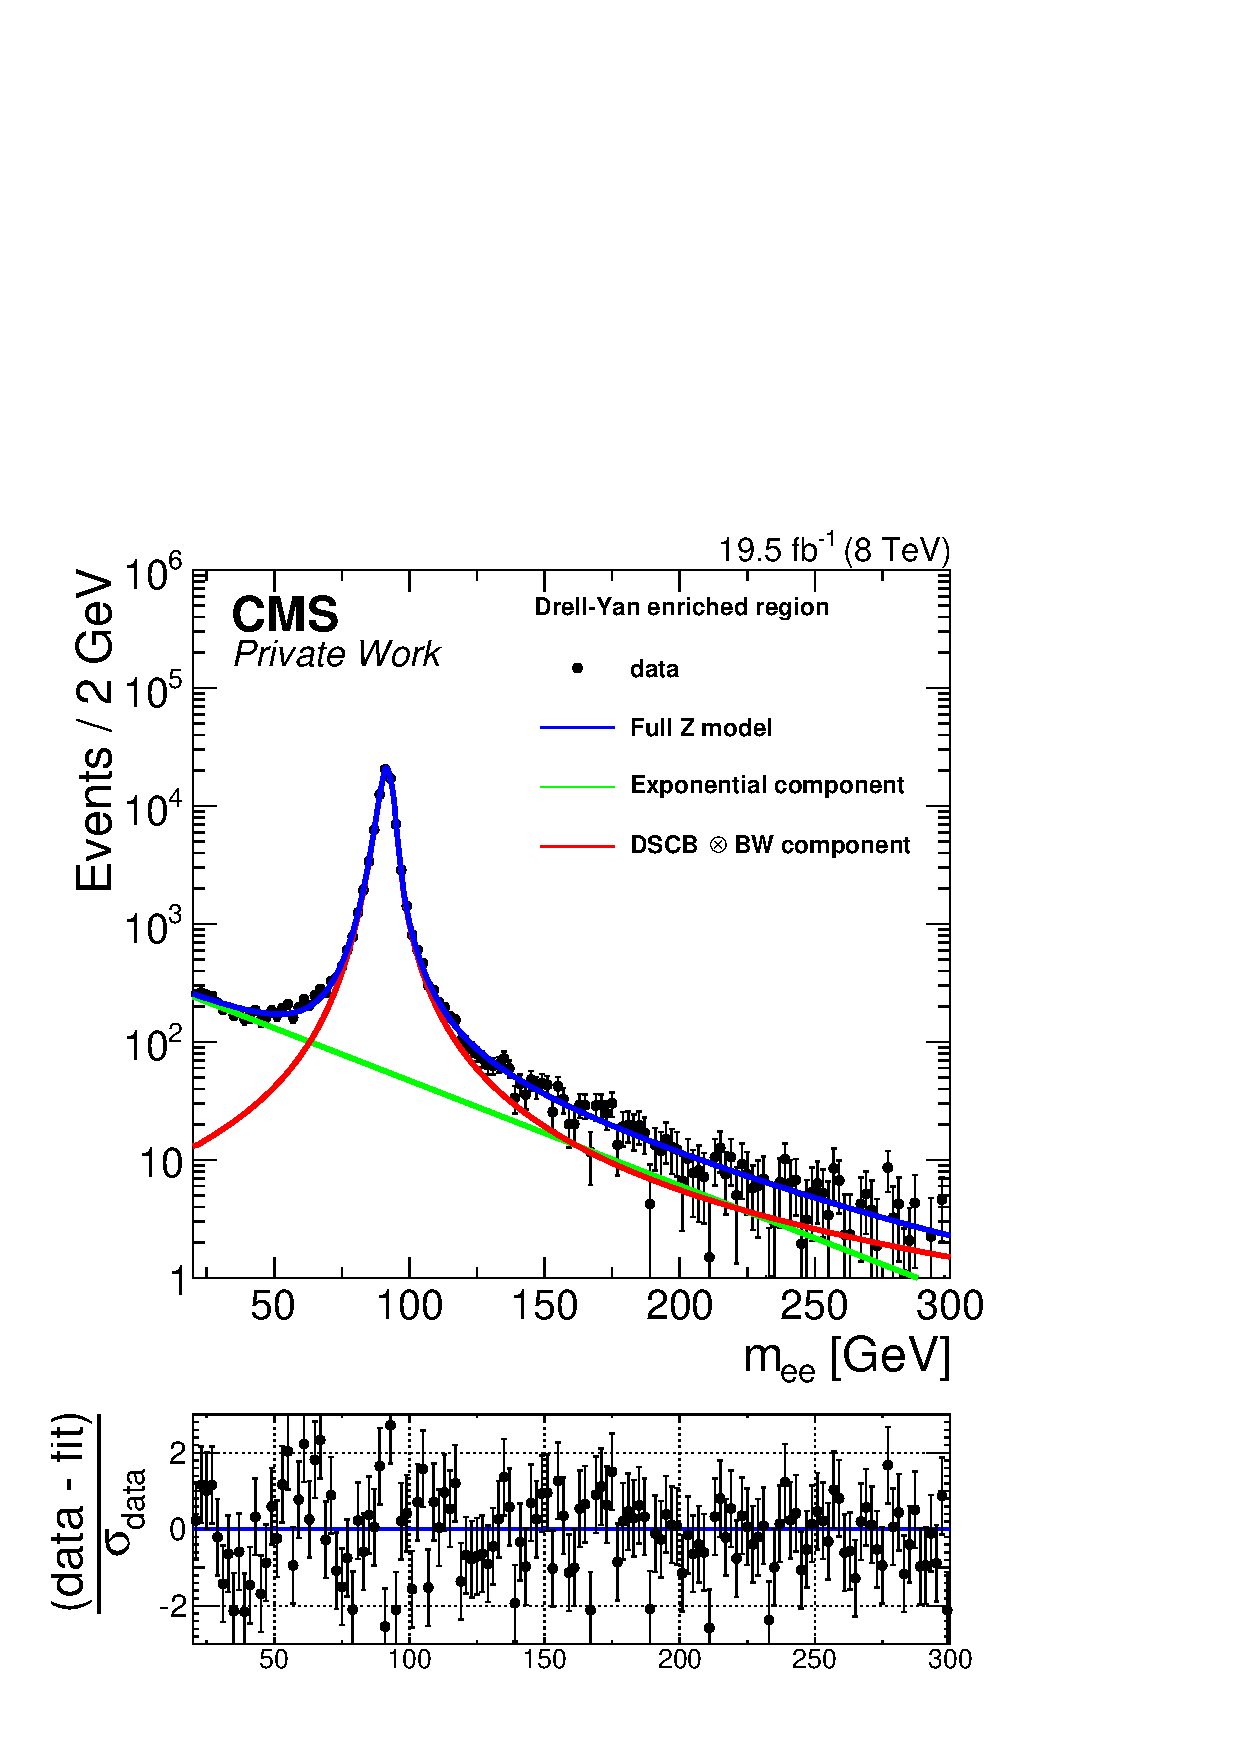
\includegraphics[width=\textwidth]{plots/results/fit/expoFitEE_Log_Central.pdf}
\end{minipage}
\begin{minipage}[t]{0.49\textwidth}
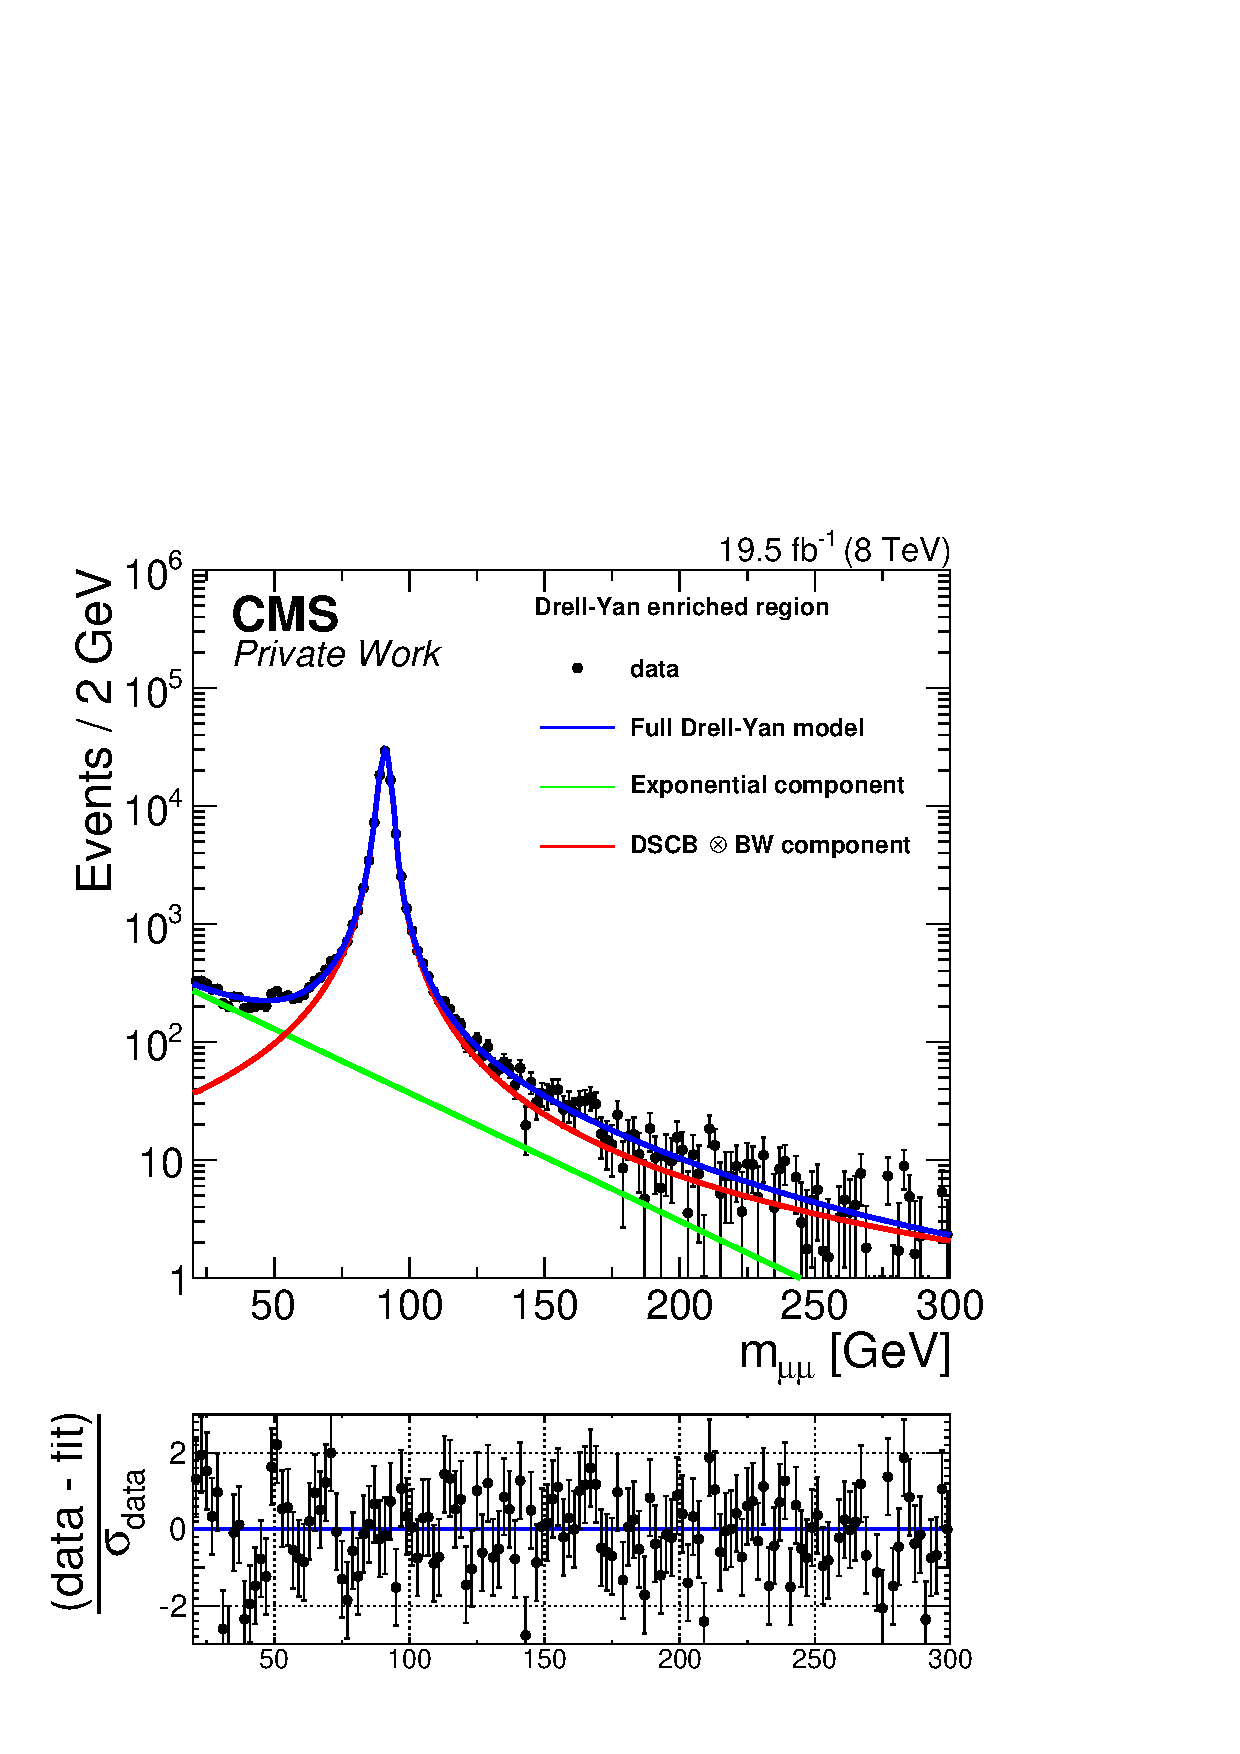
\includegraphics[width=\textwidth]{plots/results/fit/expoFitMM_Log_Central.pdf}
\end{minipage}
\begin{minipage}[t]{0.49\textwidth}
  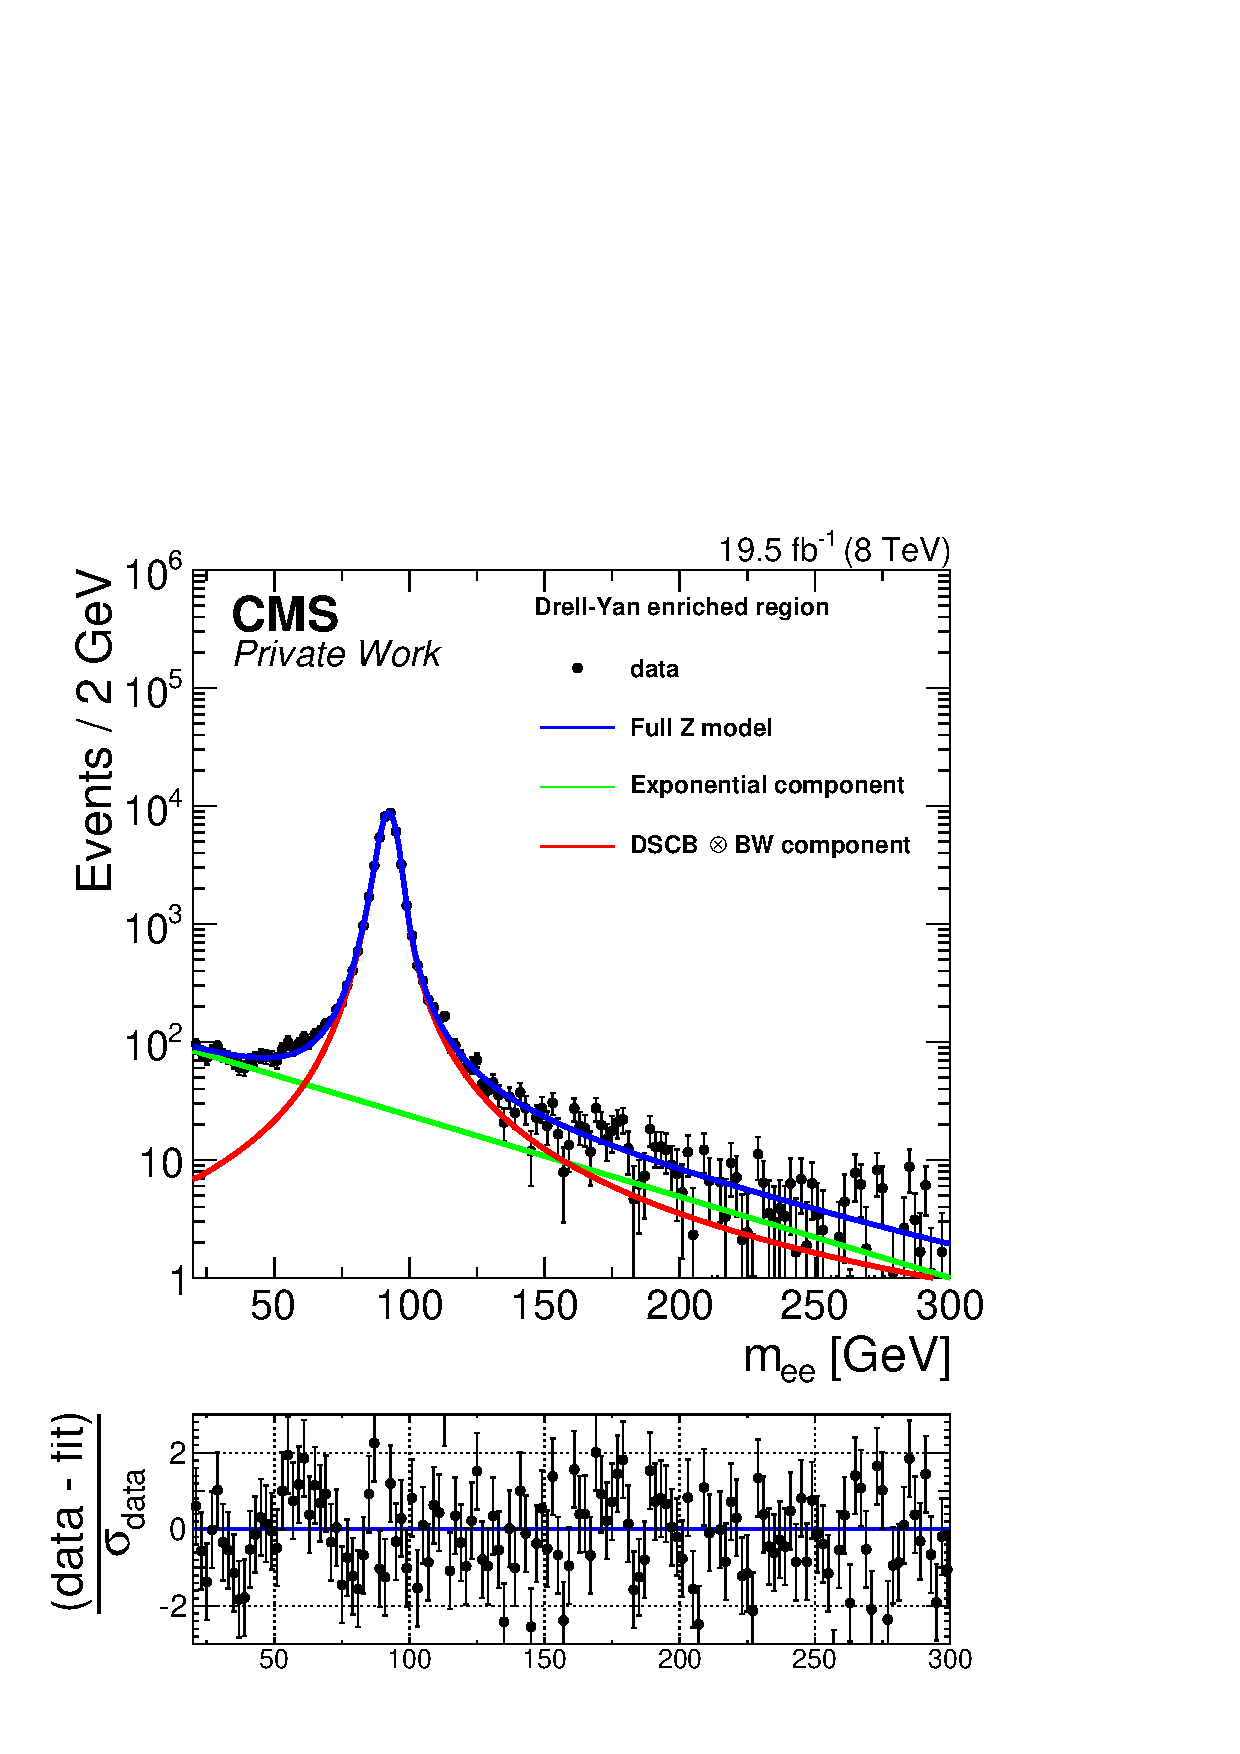
\includegraphics[width=\textwidth]{plots/results/fit/expoFitEE_Log_Forward.pdf}
\end{minipage}
\begin{minipage}[t]{0.49\textwidth}
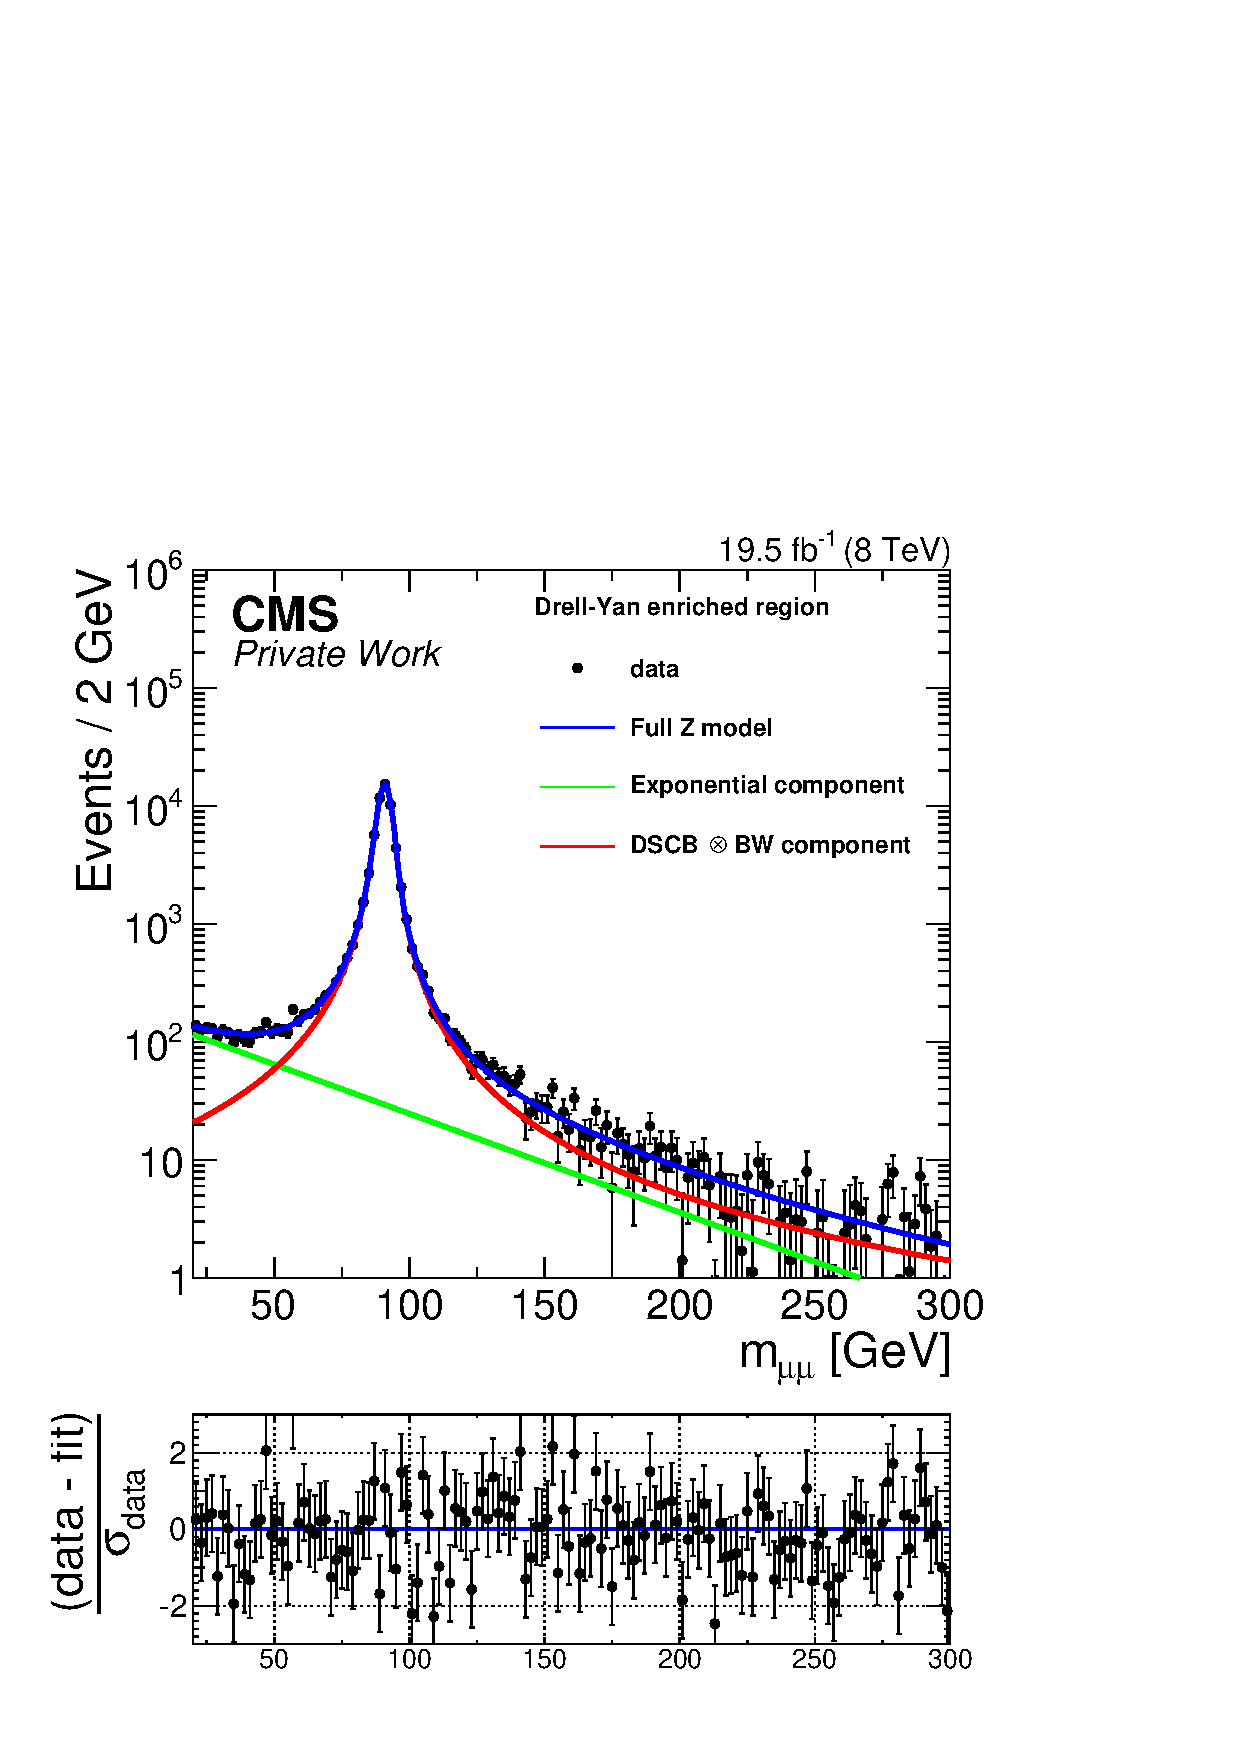
\includegraphics[width=\textwidth]{plots/results/fit/expoFitMM_Log_Forward.pdf}
\end{minipage}
\caption{Fit to the \mll distribution in the Drell--Yan control region separately for \EE (left) and \MM (right) events in the central (top) and forward (bottom) dilepton selection. The data is shown as black points while the resulting fit is shown in blue. The red and green lines show the contributions of the continuum model and the convolution of the Breit-Wigner with the double-sided crystal ball to the combined fit.}
\label{fig:dyFits}
\end{figure}
From the Gaussian core component of the double-sided crystal ball the \mll resolution $\sigma_{CB}$ in the different channels is obtained, which is used in the modelling of a potential signal. The resulting resolution values are shown in Table~\ref{tab:mllReso}. The fitted values range from about $\unit{1.4}{\giga\electronvolt}$ to $\unit{2.7}{\giga\electronvolt}$ depending on lepton flavour and rapidity. In general it is smaller for \MM pairs and for lepton pairs in the central part of the detector.  

\begin{table}
\centering
\caption{Fitted \mll resolution in the central and forward dilepton selections for \EE and \MM pairs.}
\label{tab:mllReso}
\begin{tabular}{l|c|c}
 & \EE & \MM \\
 \hline
 Central & $\unit{1.71\pm0.03}{\giga\electronvolt}$  & $\unit{1.44\pm0.01}{\giga\electronvolt}$\\
 Forward & $\unit{2.70\pm0.04}{\giga\electronvolt}$ & $\unit{2.01\pm0.03}{\giga\electronvolt}$\\

\end{tabular}
\end{table}

\subsection{Model for flavour-symmetric backgrounds}
The flavour-symmetric model accounts for most of the events in the signal region. To ensure the validity of the chosen parametrisation, a variety of alternative models are studied. Here the nominal parametrisation used in the final result is discussed followed by a description of alternatives that are used as cross-checks.
\subsubsection{Nominal parametrisation}
The nominal flavour-symmetric model consists of three parts: The rising flank of the distribution is modelled by a power law, the peak region with a third order polynomial and the falling flank with an exponential fall-off. 
\begin{eqnarray*}
{\mathcal{P}}_{FS}(m_{\ell\ell}) = \begin{cases} {\mathcal{P}}_{FS,1}(m_{\ell\ell}) = c_{1} \cdot m_{\ell\ell}^{\alpha} &\mbox{if } 20\GeV < m_{\ell\ell} < m_{\ell\ell}^{(1)} \\
{\mathcal{P}}_{FS,2}(m_{\ell\ell}) = \sum_{i=0}^{3} c_{2,i} \cdot m_{\ell\ell}^{i} & \mbox{if } m_{\ell\ell}^{(1)}<m_{\ell\ell}<m_{\ell\ell}^{(2)} \\
{\mathcal{P}}_{FS,3}(m_{\ell\ell}) = c_{3}\cdot e^{-\beta m_{\ell\ell}} & \mbox{if } m_{\ell\ell}^{(2)}<m_{\ell\ell}<300\GeV \\
\end{cases} 
\end{eqnarray*}
where $m_{\ell\ell}^{(1)}$ and $m_{\ell\ell}^{(2)}$ are the transition points between the different parts of the model. The model is required to be normalised and also to be continuously differentiable in \mll at $m_{\ell\ell}^{(1)}$ and $m_{\ell\ell}^{(2)}$, reducing the number of free parameters to five. A full list of the parameters and their properties is given in Table~\ref{tab:Fit_Par_Overview_FS}.

\begin{table}[htbp]
\begin{center}
 \renewcommand{\arraystretch}{1.3}
 \caption{List of all parameters of the nominal model for flavour-symmetric backgrounds. Given are intial values, allowed ranges and the type of the parameters. Sets of these parameters exists for both the central and forward dilepton selection.\label{tab:Fit_Par_Overview_FS}}
\begin{tabular}{l|c|c|c|c|ccccccccccccccccccccc}
& parameter & type & initial value & minimum & maximum \\ \hline
\multirow{5}{*}{$\mathbf{p}_{FS}$} & $m_{\ell\ell}^{(1)} [\mathrm{GeV}]$ & floating & 50 & 20 & 80 \\ 
& $m_{\ell\ell}^{(2)}  [\mathrm{GeV}]$ & floating & 120 & 100 & 160 \\
& $c_{2,0}$ & floating & -1800 & -5000 & 5000 \\ 
& $c_{2,1}$ & floating & 120 & -400 & 400 \\
& $c_{2,2}$ & fixed & -1 & - & - \\
& $c_{2,3}$ & floating & 2.5$\cdot10^{-3}$ & 1$\cdot10^{-4}$ & 1$\cdot10^{-2}$ \\
& $c_{1},\alpha,c_3,\beta$ & expressed in terms of $c_{2,i}$  & - & - & - \\
\end{tabular}

\end{center}
\end{table}
\subsubsection{Parametrisation from 2011 analysis}
In a previous version of the analysis~\cite{edge2011}, the following parametrisation was used : 
\begin{equation}
\label{eq:2011}
 \mathcal{P}_{FS}(m_{\ell\ell}) = c_{1} m_{\ell\ell}^{\alpha} e^{-\beta m_{\ell\ell}}
\end{equation}
It was found to be an unsatisfying description of the distribution of flavour-symmetric backgrounds after lepton \pt cuts had been raised with respect to the analysis of the 2011 dataset, but is still a useful tool for fit performance studies, as the low number of parameters reduces the runtime of the fit, allowing for tests using a large number of simulated datasets.
\subsubsection{Sum of three Gaussians}
Additionally, a sum of three Gaussians can be chosen as an analytical parametrisation of the flavour-symmetric backgrounds. The free parameters of the shape are the means $\mu_i$ and widths $\sigma_i$ of the Gaussians.
\begin{equation*}
\mathcal{P}_{FS}(m_{\ell\ell}) = \mathrm{Gauss}(\mu_1,\sigma_1) + \mathrm{Gauss}(\mu_2,\sigma_2) + \mathrm{Gauss}(\mu_3,\sigma_3)\\
\end{equation*}
The shape is found to describe the flavour-symmetric background well and to be in good agreement with the nominal parametrisation.
\subsubsection{Binned Subtraction}
\label{shapesubtraction:binnedsubtraction}
As an alternative to the analytical functions, the binned dilepton-mass distribution in the OF channel is directly used as  template of the distribution of flavour-symmetric backgrounds in the same-flavour channels. However, the normalization of this background is still determined by the simultaneous fit, taking into account the \Rsfof correction factor.

This approach has the advantage of not needing any prior knowledge on the shape of the flavour-symmetric background. It is, however, more susceptible to statistical fluctuations, as they are not smoothed out as in analytical models (for a smoothed approach see below). In order to minimise the impact of these fluctuations, a bin width of 5\GeV is chosen. This method is not suited to provide quantitative results because the statistical uncertainties on the shape are not considered in the fit, after it has been fixed by the OF data.
\subsubsection{Smoothed Subtraction}
Similarly to the binned subtraction, the opposite flavour data distribution is directly used to predict the background shape in the same flavour distribution using a kernel density estimator (KDE). The shape is constructed as a sum of Gaussian distributions, one for each event in the considered dataset with the mean set to the \mll value of that event. The implementation of one-dimensional kernel probability density functions (pdfs) in RooFit is used (\emph{RooKeysPdf} class). The probability density function for a sample of a random variable of size $n$ is estimated by a kernel density

\begin{equation*}
\hat{f}_h(\mll) = \frac{1}{nh}\sum\limits_{i=1}^n K\left(\frac{\mll-m_{\ell\ell,i}}{h}\right).
\end{equation*}
Here $K$ is the so called kernel, for which a Gaussian distribution is chosen in this analysis, and $h$ is a smoothing parameter~\cite{kernelDensity}. The width of the Gaussians is adapted depending on the density of events at a given point, using narrow widths were the density is high to preserve details of the distribution and larger widths where the density is low to assure the smoothness of the resulting shape estimate. For both the low-$m_{\ell\ell}$ and the high-$m_{\ell\ell}$ border, parts of the Gaussians extending beyond the considered range of \mll are reflected into the considered range to achieve the correct integral. Again, this method is not suited to provide quantitative results because no uncertainties on the background shape can be included, as it has to be fixed on the OF data before the combined fit can be performed.

\subsection{Signal model}
\label{sec:sigModel}
The signal is modelled by a triangular shape convolved with a Gaussian distribution, which will be shown to be a good approximation of the actual, model dependent, shape. The width of the Gaussian $\sigma_{\ell\ell}$ depends on the detector resolution in the corresponding channel and is obtained from the fit to the \Z boson peak in the Drell--Yan control region described in Section~\ref{sec:Zmodel}. The model can be parametrised as
\begin{equation*}
 {\mathcal{P}}_{S}(m_{\ell\ell}) = \frac{1}{\sqrt{2\pi\sigma_{\ell\ell}^2}} \int_{0}^{m_{\ell\ell}^{edge}} y \cdot \textrm{exp}\left( -\frac{(m_{\ell\ell}-y)^2}{2\sigma_{\ell\ell}^{2}}\right) dy,
\end{equation*}
with the endpoint of the triangle $m_{\ell\ell}^{edge}$ as the only free parameter, as the starting point is always $\unit{0}{\giga\electronvolt}$.

To cross-check the dependence of the results on the parametrisation of the signal, two additional signal shapes with strongly differing shapes are defined. Here, the linear rise of the triangle is replaced by different dependencies on \mll, depending on the sign of the exponent $\gamma$. This results in concave and convex shapes instead of the simple triangle:

\begin{equation}
\label{eq:convex}
 {\mathcal{P}}^{\text{convex}}_{S}(m_{\ell\ell}) = \frac{1}{\sqrt{2\pi\sigma_{\ell\ell}^2}} \int_{0}^{m_{\ell\ell}^{edge}} y^{\gamma} \cdot \textrm{exp}\left( -\frac{(m_{\ell\ell}-y)^2}{2\sigma_{\ell\ell}^{2}}\right) dy,
\end{equation}

\begin{equation}
\label{eq:concave}
 {\mathcal{P}}_{S}^{\text{concave}}(m_{\ell\ell}) = \frac{1}{\sqrt{2\pi\sigma_{\ell\ell}^2}} \int_{0}^{m_{\ell\ell}^{edge}} \left(\left(m_{\ell\ell}^{edge}\right)^{\gamma} -\left(y-m_{\ell\ell}^{edge}\right)^{\gamma}\right) \cdot \textrm{exp}\left( -\frac{(m_{\ell\ell}-y)^2}{2\sigma_{\ell\ell}^{2}}\right) dy.
\end{equation}
A comparison of the three types of signal shapes is shown in Figure~\ref{fig:mc:shapes} for for $m_{\ell\ell}^{edge} = \unit{75}{\giga\electronvolt}$ and $\sigma_{\ell\ell} = \unit{1.5}{\giga\electronvolt}$. To make the differences between the shapes clearly visible, in the case of the convex and concave signal shapes a value of $\gamma = 4$ has been chosen. The convex shape is peaked towards the endpoint of the distribution while the concave shape leads to a significant signal contribution at much lower values of \mll compared to the nominal triangular shape. Nevertheless, all three shapes exhibit the striking edge at \mlledge.
\begin{figure}[tbp]
\centering
  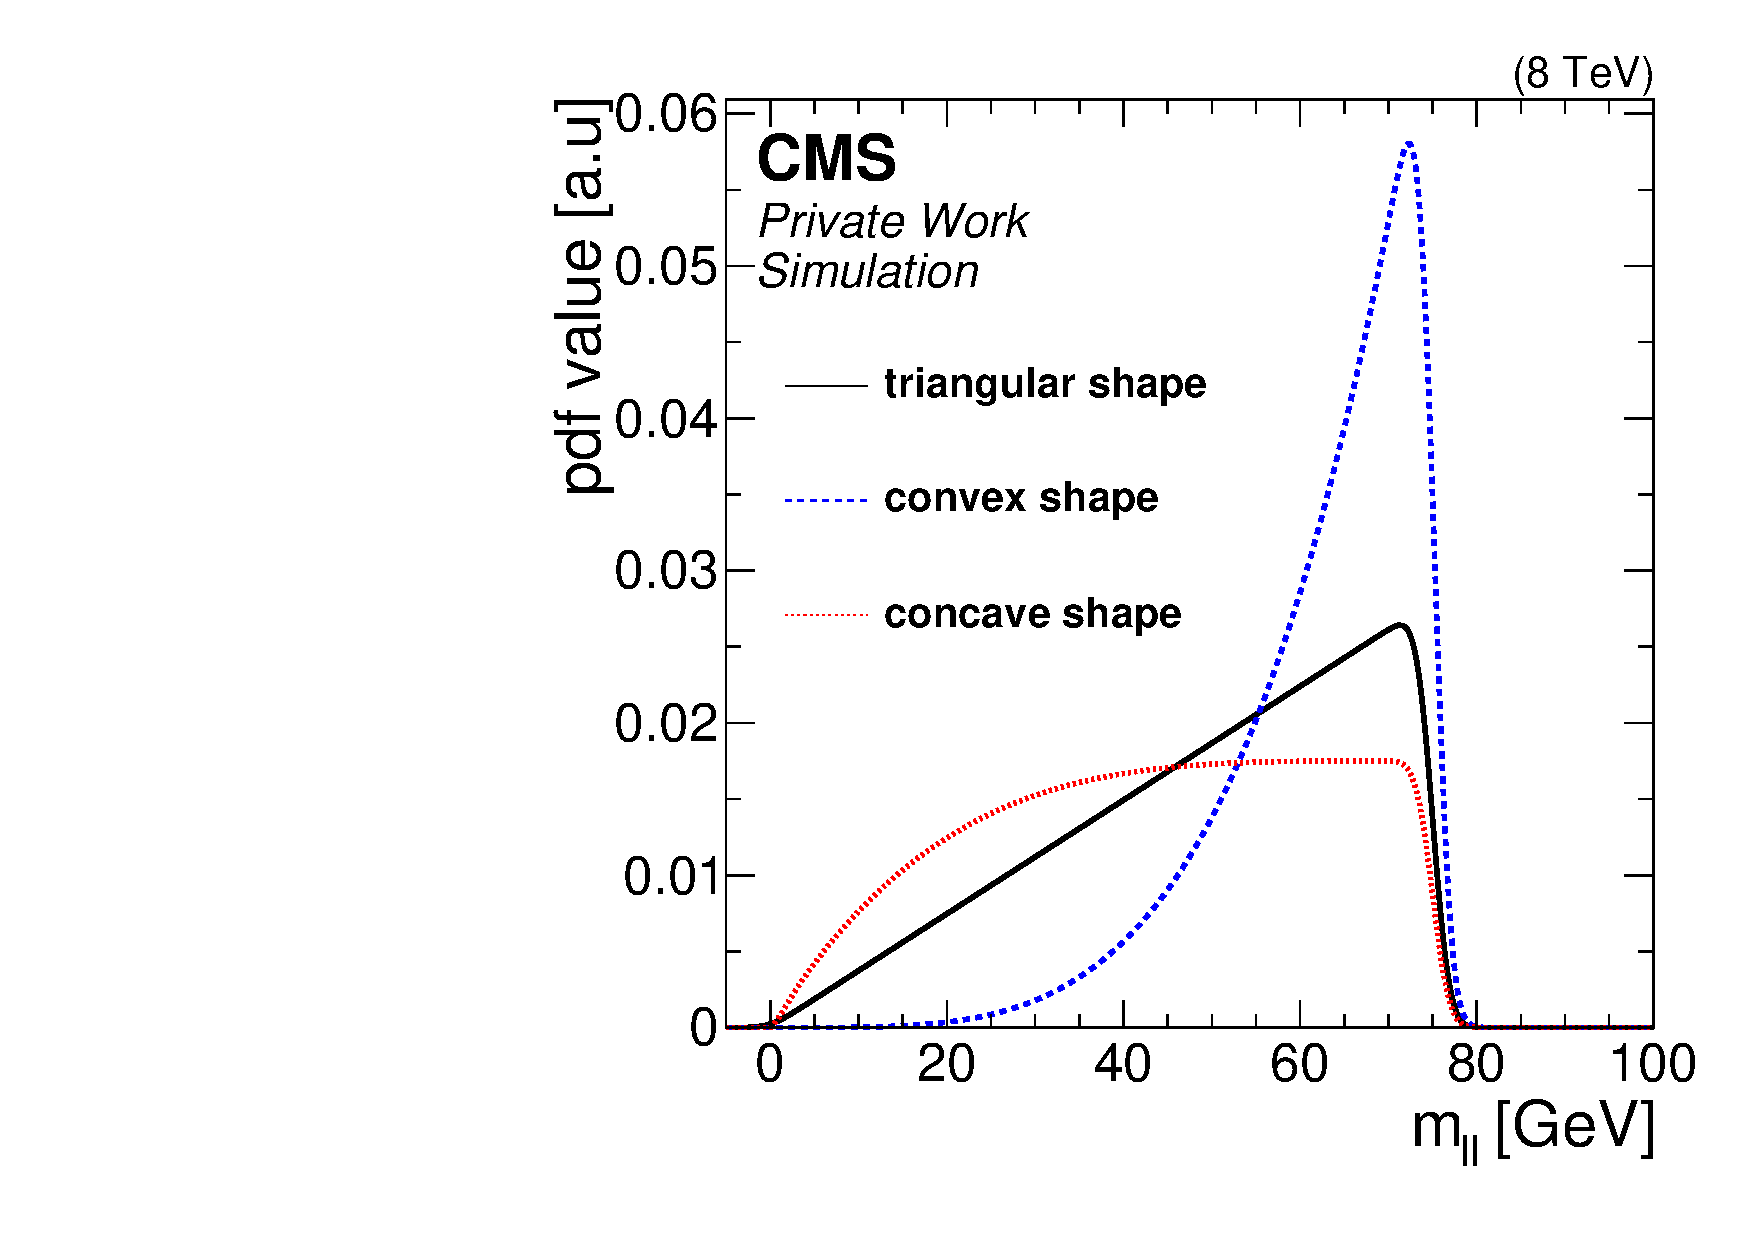
\includegraphics[width=0.6\textwidth]{plots/results/fit/shapes.pdf}
\caption{Illustration of the three different signal shapes for $m_{\ell\ell}^{edge} = \unit{75}{\giga\electronvolt}$ and $\sigma_{\ell\ell} = \unit{1.5}{\giga\electronvolt}$. In the case of the convex and concave signal shapes, a value of $\gamma = 4$ has been chosen.}
\label{fig:mc:shapes}
\end{figure}

The parameters of the signal model are listed in Table~\ref{tab:Fit_Par_Overview_Sig}.
\begin{table}[b]
\begin{center}
 \renewcommand{\arraystretch}{1.3}
 \caption{List of all parameters of the nominal signal model. Given are intial values, allowed ranges and the type of the parameters. Sets of these parameters exists for both the central and forward dilepton selection.\label{tab:Fit_Par_Overview_Sig}}
\begin{tabular}{l|c|c|c|c|ccccccccccccccccccccc}
& parameter & type & initial value & minimum & maximum \\ \hline
\multirow{2}{*}{$\mathbf{p}_{S}^{ee}$} & $m_{\ell\ell}^{edge} [\mathrm{GeV}]$ & floating & varying & 30 & 300 \\ 
& $\sigma_{CB}^{ee}  [\mathrm{GeV}]$ & fixed & see Table~\ref{tab:mllReso} & - & - \\ \hline
\multirow{2}{*}{$\mathbf{p}_{S}^{\mu\mu}$} & $m_{\ell\ell}^{edge} [\mathrm{GeV}]$ & floating & varying & 30 & 300 \\ 
& $\sigma_{CB}^{\mu\mu}  [\mathrm{GeV}]$ & fixed & see Table~\ref{tab:mllReso} & - & - \\
\end{tabular}

\end{center}
\end{table}

The signal model is fitted to simulation using four parameter points of the fixed-edge and slepton-edge models described in Section~\ref{sec:models}. The points are chosen to study edges produced in decays both via an off-shell \Z boson and sleptons and also to test the fit performance for edge positions below, on, and above the \Z boson peak. The signal parameters are summarised in Table~\ref{tab:signals} and will be referenced by their labels S1-S4 in the following.

\begin{table}[htbp]

\begin{center}
 \renewcommand{\arraystretch}{1.3}
\caption{Overview of the benchmark signal points used in fit performance studies.\label{tab:signals}}

\begin{tabular}{l|c|c|c|c}
 name & S1 & S2 & S3 & S4 \\ \hline
model & fixed-edge & slepton-edge & slepton-edge & slepton-edge \\
$m_{\sbottom}$ [GeV]   & 400 & 500  & 500  & 450 \\
$m_{\secondchi}$ [GeV] & 150 & 175  & 200  & 275\\
$m_{\firstchi}$ [GeV]  & 80  & 100  & 100  & 100\\
gen. \mlledge [GeV]    & 70  & 74.3 & 98.6 & 170.2 \\

\end{tabular}
\end{center}
\end{table}

If more than two leptons are reconstructed in an event, the wrong combination might be chosen, leading to a flavour-symmetric, background-like contribution of the signal. This happens more often in the slepton-edge model because of the much higher branching fraction into leptons. Therefore, a model for flavour-symmetric backgrounds is also fitted to the signal. For these tests, the KDE shape is used because of its fast convergence. 

Fits to the fixed-edge model points S1 are shown in Figure~\ref{fig:signalModel:edge}. After subtraction of the very small flavour-symmetric contribution, this model predicts about 122 events in the central and 15 events in the forward region with an edge position of $\unit{70}{\giga\electronvolt}$, in agreement with the expectation that the decay products of heavy SUSY particles are located dominantly in the central region of the detector. In the upper plots fits are shown using the nominal triangular shape. It is clearly not a good approximation of the actual shape of the signal because it does not describe the peak towards the \Z boson mass, which is present because the decay of the \secondchi occurs exclusively via an off-shell \Z boson. However, the signal parameters \mlledge and $N_S$ are still reproduced very well. In the lower two plots, the convex signal shape was used, with the exponent $\gamma$ as a free parameter. The resulting shape is a much better description of the signal, with a fitted $\gamma$ of about 2.62. However, no significant change in the other signal parameters is observed. 

\begin{figure}[hbp]
  \centering
  \begin{minipage}[t]{0.49\textwidth}
    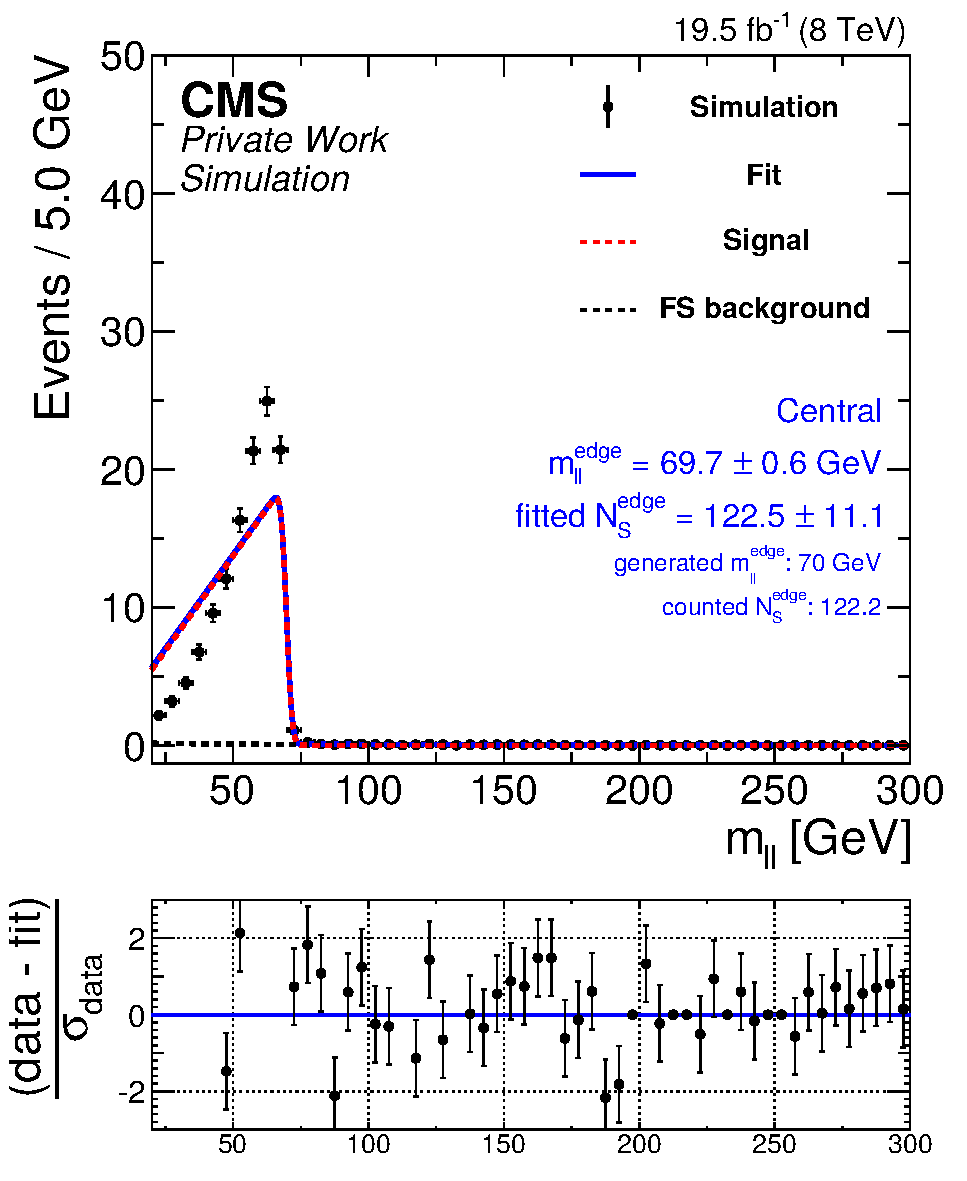
\includegraphics[width=\textwidth]{plots/results/fit/mcFits/shapeIllustrationKTriangle_SignalInclusive_Combined_Full2012_KTriangle_MC_edge_400_150_80_Central.pdf}
  \end{minipage}
  \begin{minipage}[t]{0.49\textwidth}
    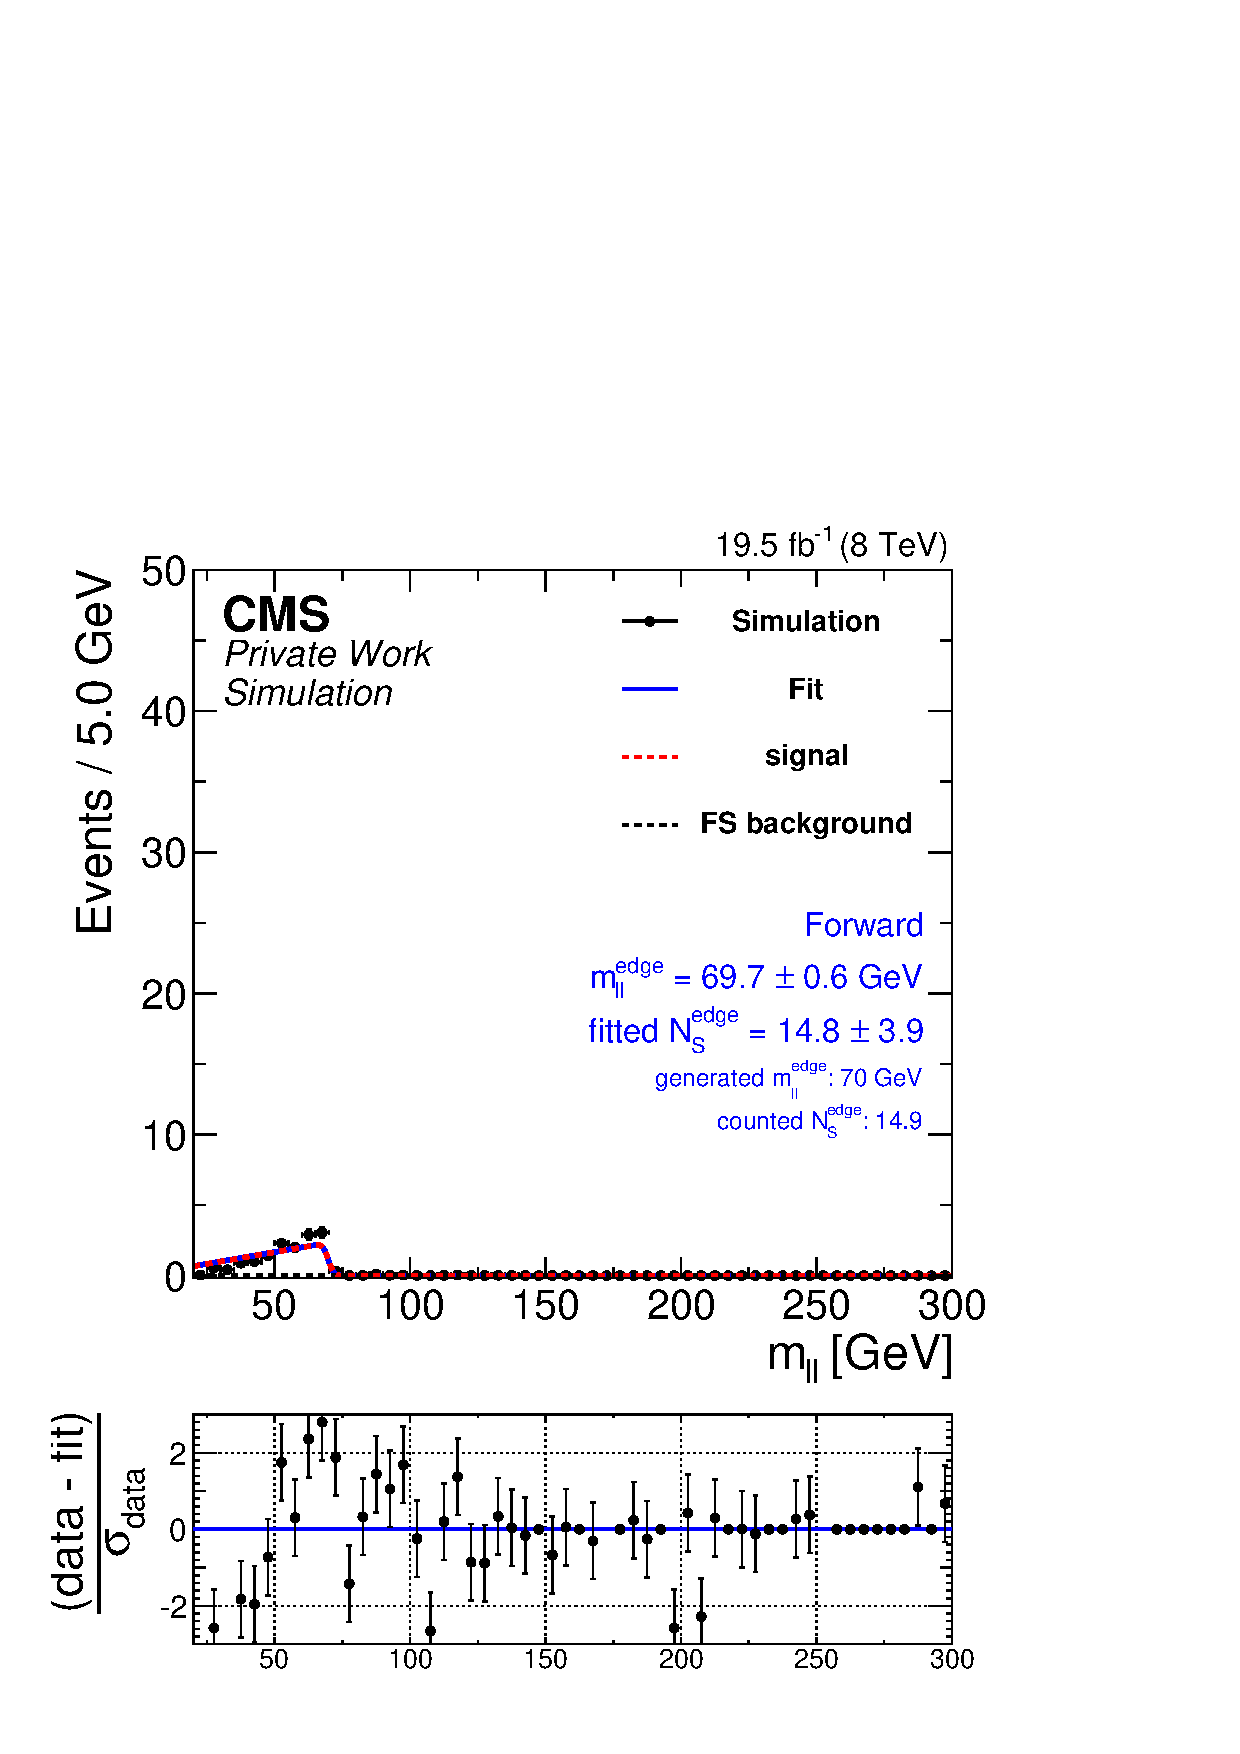
\includegraphics[width=\textwidth]{plots/results/fit/mcFits/shapeIllustrationKTriangle_SignalInclusive_Combined_Full2012_KTriangle_MC_edge_400_150_80_Forward.pdf}
  \end{minipage}
  \begin{minipage}[t]{0.49\textwidth}
    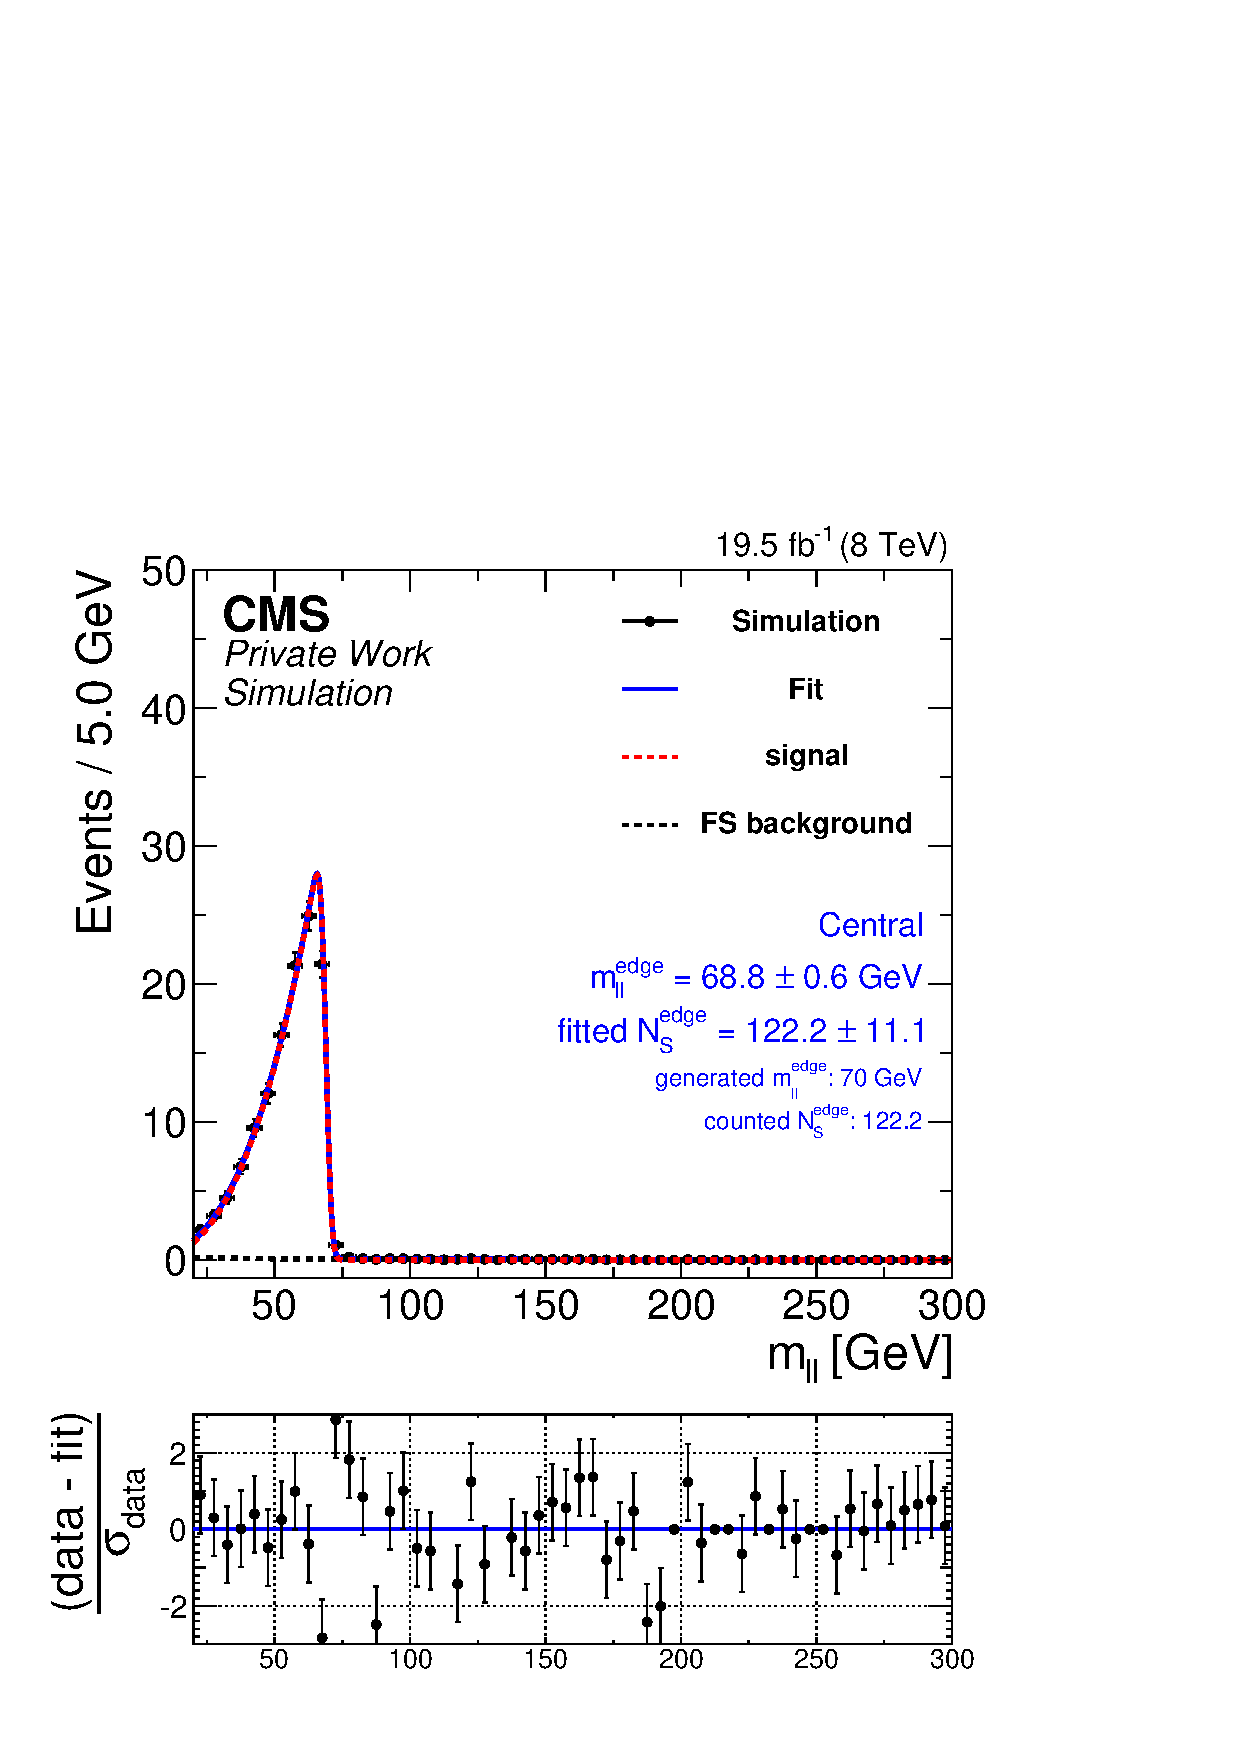
\includegraphics[width=\textwidth]{plots/results/fit/mcFits/shapeIllustrationKX4_SignalInclusive_Combined_Full2012_KX4_MC_edge_400_150_80_Central.pdf}
  \end{minipage}
  \begin{minipage}[t]{0.49\textwidth}
    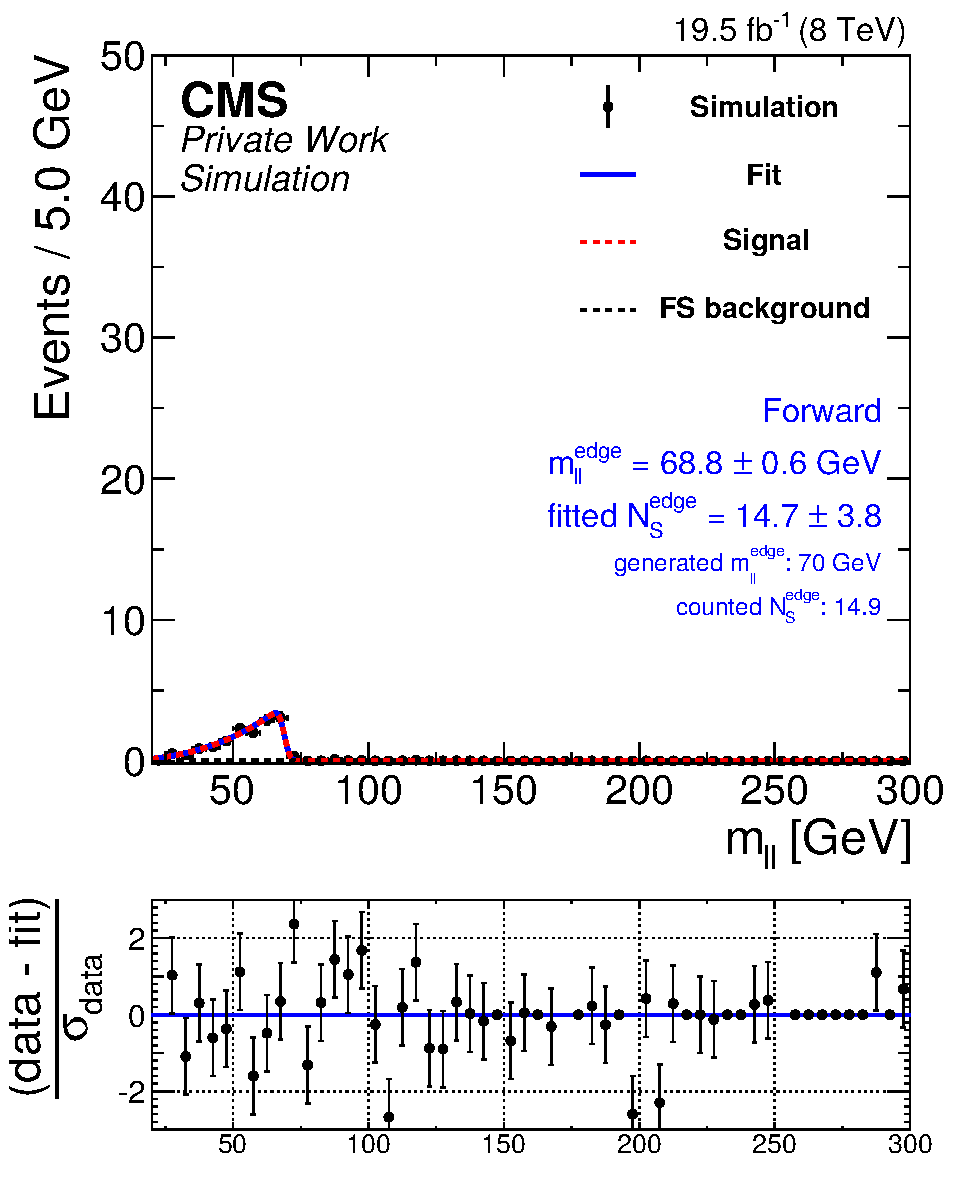
\includegraphics[width=\textwidth]{plots/results/fit/mcFits/shapeIllustrationKX4_SignalInclusive_Combined_Full2012_KX4_MC_edge_400_150_80_Forward.pdf}
  \end{minipage}
  \caption{Fit of the signal model to the fixed-edge model S1 (see Table~\ref{tab:signals}). Shown are fits with the nominal triangular shape (top) and the convex shape (bottom), for which the exponent $\gamma$ is left floating, in both the central (left) and forward (right) signal regions.}
  \label{fig:signalModel:edge}
\end{figure}

In Figure~\ref{fig:signalModel:slepton} a fit to the slepton-edge model point S2 is shown. As the decays occur dominantly via an intermediate slepton, the triangular shape is a much better approximation of the signal shape. Because of the much higher branching fraction into leptons of this model, a significant flavour-symmetric contribution due to combinatorics is present, which is accounted for by the background description and reduces the observable signal yield. Again, the signal parameters are well reproduced by the fit. Similar performance is also observed for the points S3 and S4. 

\begin{figure}[t]
  \centering
  \begin{minipage}[t]{0.49\textwidth}
    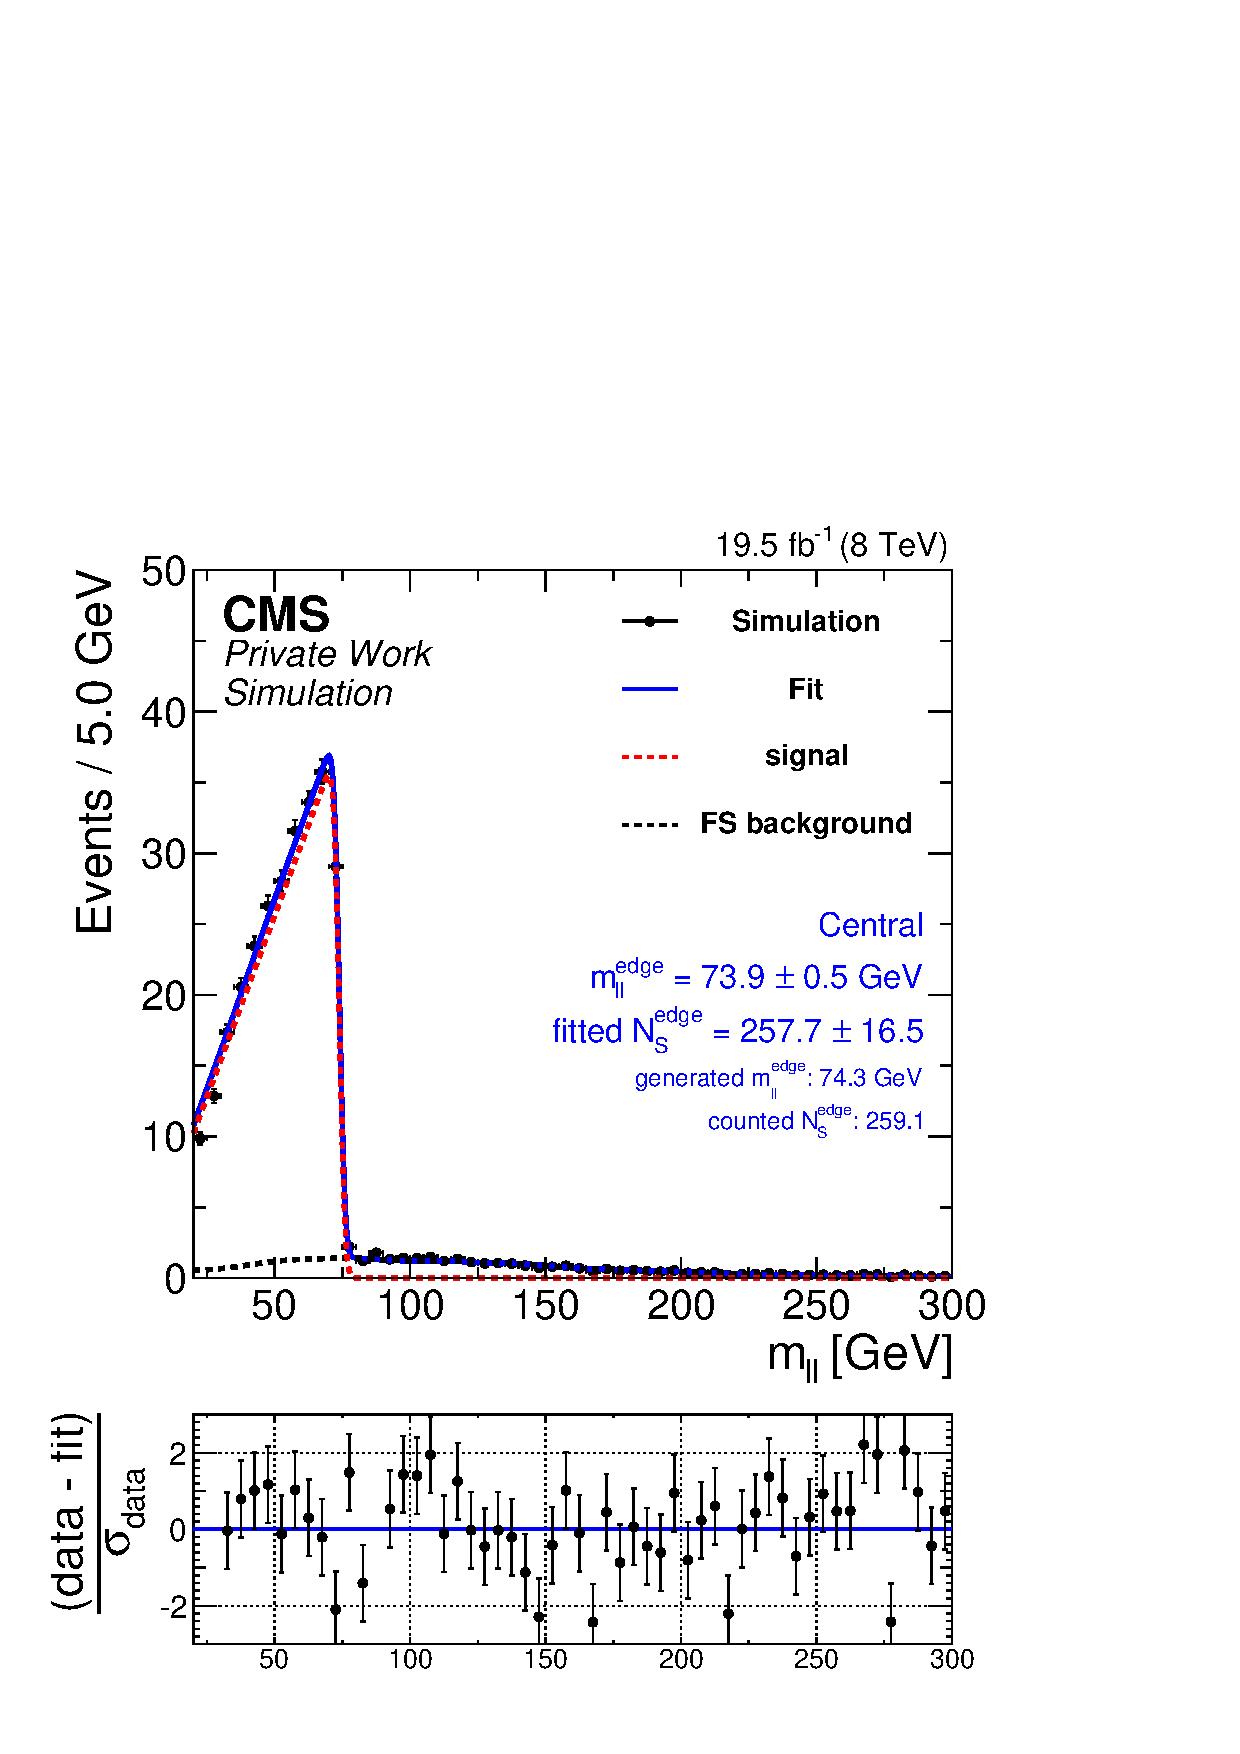
\includegraphics[width=\textwidth]{plots/results/fit/mcFits/shapeIllustrationKTriangle_SignalInclusive_Combined_Full2012_KTriangle_MC_slepton_500_175_100_Central.pdf}
  \end{minipage}
  \begin{minipage}[t]{0.49\textwidth}
    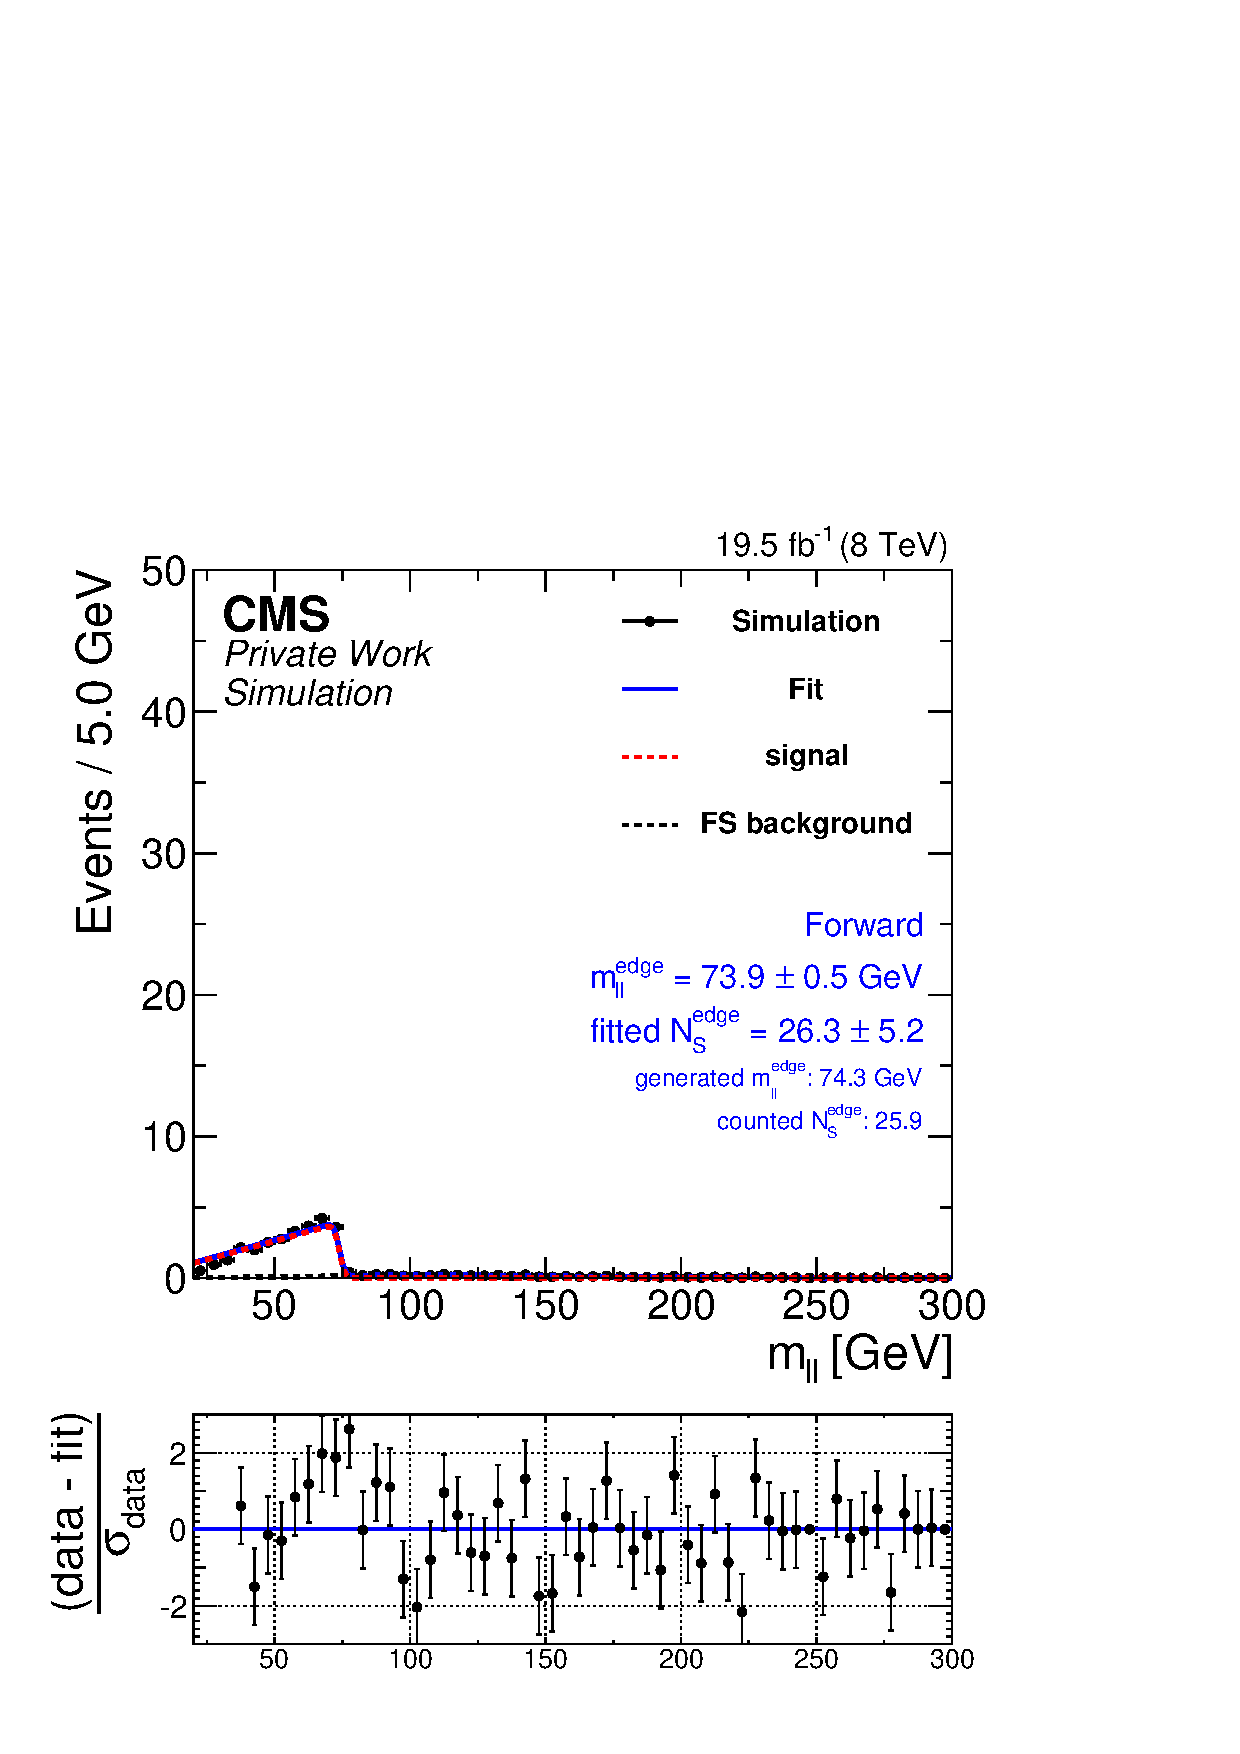
\includegraphics[width=\textwidth]{plots/results/fit/mcFits/shapeIllustrationKTriangle_SignalInclusive_Combined_Full2012_KTriangle_MC_slepton_500_175_100_Forward.pdf}
  \end{minipage}
\caption{Fit of the signal model to the slepton-edge model S2 (see Table~\ref{tab:signals}). Shown are fits in both the central (left) and forward (right) signal regions.}
  \label{fig:signalModel:slepton}
\end{figure}


\section{Combined model}
\label{sec:fullModel}
The full models fitted to the different event categories are constructed by adding yield parameters $N_x$ for each component. For opposite flavour events, the model is simply given by 
\begin{equation*}
 \mathcal{P}_{OF}(m_{\ell\ell}) = N_{FS} \cdot \mathcal{P}_{FS}(m_{\ell\ell}).
\end{equation*}
For \EE and \MM events, also yield parameters for the Drell--Yan background and the signal models have to be introduced. 
\begin{eqnarray*}
 {\mathcal{P}}_{ee}(m_{\ell\ell})     & = &  N_{FS}^{ee} \cdot {\mathcal{P}}_{FS}(m_{\ell\ell})      +  N_{Z}^{ee} \cdot {\mathcal{P}}_{Z,ee}(m_{\ell\ell})           +   N_{S}^{ee} \cdot  {\mathcal{P}}_{S}(m_{\ell\ell},\sigma_{ee}) \\
 {\mathcal{P}}_{\mu\mu}(m_{\ell\ell}) & = &   N_{FS}^{\mu\mu} \cdot {\mathcal{P}}_{FS}(m_{\ell\ell})  +  N_{Z}^{\mu\mu} \cdot {\mathcal{P}}_{Z,\mu\mu}(m_{\ell\ell})   +   N_{S}^{\mu\mu} \cdot {\mathcal{P}}_{S}(m_{\ell\ell},\sigma_{\mu\mu}) \\
\end{eqnarray*}
As the lepton efficiencies do not depend on the origin of the leptons and the branching fraction of the decays into electrons or muons is the same for both the backgrounds and the considered fixed-edge and slepton-edge models, the number of free parameters can be reduced by assuming an universal fraction of \EE events in both background and signal, which is expressed as $0 < f_{ee} < 1$. Also, the flavour-symmetric yields in the two SF channels are connected to that in the OF channel via \Rsfof, which allows to construct the following relations:
\begin{center}
  \begin{minipage}[t]{0.49\textwidth}
\begin{eqnarray*}
 N_{S}^{ee} &=& f_{ee} \cdot N_{S}, \\
  N_{Z}^{ee} &=& f_{ee} \cdot N_{Z},\\
    N_{FS}^{ee} &=& f_{ee} \cdot \Rsfof \cdot N_{FS}, \\
\end{eqnarray*}
  \end{minipage}
  \begin{minipage}[t]{0.49\textwidth}
\begin{eqnarray*}
 N_{S}^{\mu\mu} &=& (1-f_{ee}) \cdot N_{S}, \\
  N_{Z}^{\mu\mu} &=& (1-f_{ee}) \cdot N_{Z}, \\
    N_{FS}^{\mu\mu} &=& (1-f_{ee}) \cdot \Rsfof \cdot N_{FS}. \\
\end{eqnarray*}
  \end{minipage}
\end{center}
The systematic uncertainty on \Rsfof is included in the fit as a constraint in the form of a Gaussian function with mean and width set to the values measured in Section~\ref{sec:combinedRSFOF}:
\begin{equation*}
\mathrm{Gauss}\left(\Rsfof;\Rsfof^{\text{measured}},\sigma_{\Rsfof}^{\text{measured}}\right).
\end{equation*}
The full likelihood of the model as a function of \mll for a given set of parameters $\mathbf{p}$ that is simultaneously fit to the unbinned data in the six channels (\EE,\MM, and OF for central and forward lepton selection) is constructed by multiplying the pdfs of the different channels and is given by

\begin{eqnarray*}
{\mathcal{L}}(m_{\ell\ell};\mathbf{p}) =&&   \prod\limits_{i\text{ } \epsilon \text{ central, forward}} \mathcal{N}_i^{ee} \times \mathcal{N}_i^{\mu\mu} \times \mathcal{N}_i^{OF}\\
                        &\times& \prod_{\EE,i}\left[N_{FS}^{ee,i} \cdot {\mathcal{P}}_{FS}^i(m_{\ell\ell};\mathbf{p}_{FS}^i) %
                                                  + N_{Z}^{ee,i} \cdot {\mathcal{P}}_{Z}^i(m_{\ell\ell};\mathbf{p}_{Z}^{ee,i}) %
                                                  + N_{S}^{ee,i} \cdot {\mathcal{P}}_{S}^i(m_{\ell\ell};\mathbf{p}_{S}^{ee,i})\right] \\
                        &\times& \prod_{\MM,i}\left[N_{FS}^{\mu\mu,i} \cdot {\mathcal{P}}_{FS}^i(m_{\ell\ell};\mathbf{p}_{FS}^i) %
                                                  + N_{Z}^{\mu\mu,i} \cdot {\mathcal{P}}_{Z}^i(m_{\ell\ell};\mathbf{p}_{Z}^{\mu\mu,i}) %
                                                  + N_{S}^{\mu\mu,i} \cdot {\mathcal{P}}_{S}^i(m_{\ell\ell};\mathbf{p}_{S}^{\mu\mu,i})\right] \\
                        &\times& \prod_{\EM,i}\left[N_{FS}^{OF,i} \cdot {\mathcal{P}}_{FS}^i(m_{\ell\ell};\mathbf{p}_{FS}^i)\right] \\   
                        &\times& {\mathrm{Gauss}^i\left(\Rsfof^i\right)}, \\
\end{eqnarray*}
where the different $\mathbf{p}^i_{x}$ denote the sets of free parameters of the models and the $\mathcal{N}_i^{\ell\ell}$ are Poisson factors describing the normalisation of the different samples. These factors take the form
\begin{equation*}
\mathcal{N}_i^{ee,\mu\mu} = \frac{(N_{FS}^{\ell\ell,i} + N_{Z}^{\ell\ell,i} + N_{S}^{\ell\ell,i})^{N_i^{\ell\ell}} e^{-(N_{FS}^{\ell\ell,i} + N_{Z}^{\ell\ell,i} + N_{S}^{\ell\ell,i})}}{N_i^{\ell\ell}!}
\end{equation*} 
for $\ell\ell = \EE, \MM$ and
\begin{equation*}
\mathcal{N}_i^{OF} = \frac{(N_{FS}^{\ell\ell,i})^{N_i^{\ell\ell}} e^{-(N_{FS}^{\ell\ell,i})}}{N_i^{\ell\ell}!}
\end{equation*}
for $\ell\ell = \EM$, with $i =$ central, forward. $N_i^{\ell\ell}$ is the number of observed events in the respective channel. 

A full overview of all parameters of the model is shown in Table~\ref{tab:Fit_Par_Overview_Full}. In total, the model has 59 parameters, of which 21 are free parameters in the signal region, 34 describe the Drell--Yan model and four are the mean values and widths of \Rsfof used in the constraints. 


\begin{table}[htbp]
\begin{center}
 \renewcommand{\arraystretch}{1.3}
 \caption{List of parameters of the full fit model. For more details on the parameter sets $\mathbf{p}_{FS}$, $\mathbf{p}_{Z}$, and $\mathbf{p}_{S}$ see Tables~\ref{tab:Fit_Par_Overview_Z},~\ref{tab:Fit_Par_Overview_FS}, and~\ref{tab:Fit_Par_Overview_Sig}. For yield parameters the initial value and allowed ranges are calculated from the observed yields $N_{SF}$ and $N_{OF}$ in the signal region for both the central (C) and forward (F) dilepton selection. \label{tab:Fit_Par_Overview_Full}}
\begin{tabular}{c|c|c|c|ccccccccccccccccccccc}
parameter & type & initial value & minimum & maximum \\ \hline
\multicolumn{5}{c}{Normalisation parameters}\\ \hline
$N_{FS}^{C}$ & floating & $0.7\cdot N_{OF}^{C}$ & 0 & $2\cdot N_{OF}^{C}$ \\
$N_{FS}^{F}$ & floating & $0.7\cdot N_{OF}^{F}$ & 0 & $2\cdot N_{OF}^{F}$ \\
$N_{S}^{C}$ & floating & 0 &  $-0.4\cdot N_{SF}^{C}$ &  $0.4\cdot N_{SF}^{C}$ \\
$N_{S}^{F}$ & floating & 0 &  $-0.8\cdot N_{SF}^{F}$ &  $0.8\cdot N_{SF}^{F}$ \\
$N_{Z}^{C}$ & floating & pred. from data & 0 & $N_{SF}^{C}(81\GeV < \mll < 101\GeV)$ \\
$N_{Z}^{F}$ & floating & pred. from data & 0 & $N_{SF}^{F}(81\GeV < \mll < 101\GeV)$ \\ \hline
\multicolumn{5}{c}{Shape parameters} \\ \hline
$\mathbf{p}_{Z}^{C}$ & mixed & \multicolumn{3}{c}{\multirow{2}{*}{see Table~\ref{tab:Fit_Par_Overview_Z}}}\\
$\mathbf{p}_{Z}^{F}$ & mixed & \multicolumn{3}{c}{}\\
$\mathbf{p}_{FS}^{C}$ & mixed & \multicolumn{3}{c}{\multirow{2}{*}{see Table~\ref{tab:Fit_Par_Overview_FS}}}\\
$\mathbf{p}_{FS}^{F}$ & mixed & \multicolumn{3}{c}{}\\
$\mathbf{p}_{S}^{C}$ & mixed & \multicolumn{3}{c}{\multirow{2}{*}{see Table~\ref{tab:Fit_Par_Overview_Sig}}}\\
$\mathbf{p}_{S}^{F}$ & mixed & \multicolumn{3}{c}{}\\ \hline
\multicolumn{5}{c}{Constraint parameters}\\ \hline
$R_{SF/OF}^{C}$ & constrained & $R_{SF/OF}^{C,\text{meas.}}$  & $R_{SF/OF}^{C,\text{meas.}}$ - $4\cdot \sigma_{R_{SF/OF}}^{C,\text{meas.}}$ & $R_{SF/OF}^{C,\text{meas.}}$ + $4\cdot \sigma_{R_{SF/OF}}^{C,\text{meas.}}$ \\
$R_{SF/OF}^{F}$ & constrained & $R_{SF/OF}^{F,\text{meas.}}$  & $R_{SF/OF}^{F,\text{meas.}}$ - $4\cdot \sigma_{R_{SF/OF}}^{F,\text{meas.}}$ & $R_{SF/OF}^{F,\text{meas.}}$ + $4\cdot \sigma_{R_{SF/OF}}^{F,\text{meas.}}$ \\
\end{tabular}

\end{center}
\end{table}


\section{Fit validation}
Before the fit is applied to data, several studies are performed to assess its performance in different scenarios. The fit is performed on simulated SM backgrounds and several benchmark signal points. As the results are subject to the fluctuations of the specific MC samples available for this study, the fit performance is furthermore studied in detail using a large number of toy datasets generated from the fit model itself. 
\subsection{Fit performance on simulation}
The ability of the fit to correctly describe different datasets is tested using the simulation of SM and signal processes described in Section~\ref{sec:MCGen}, normalized to \lumi. The full list of background processes is considered and fits are performed with and without the injection of signal points from the fixed-edge and slepton-edge models described in Section~\ref{sec:models}. To maintain an acceptable runtime of the unbinned fit, a smaller inclusive $t\bar{t}$ sample is used instead of the large samples separated into the different final states. 

The result of a fit to background-only simulation is shown in Figure~\ref{fig:mc:bgOnly}. The combined model is a good description of the simulation. A negative signal yield is fitted in both the central and forward signal region. While in the central region this is a small effect compared to the fitted uncertainty, in the forward region there is a large underfluctuation of the background at lower invariant masses, leading to a fitted signal yield of $-38\pm15$ events. To verify that this is indeed the global minimum, a scan of the log-likelihood versus \mlledge is performed. The result is shown in Figure~\ref{fig:mc:bgOnlyProfile}. Above the \Z boson peak the result is only little dependent on \mlledge. Below the peak, however, there is relatively broad minimum with a large rise directly above the global minimum, which reflects the fluctuation in the simulation in the forward region around $\unit{70}{\giga\electronvolt}$. Several relevant fit parameters in the central signal region are shown in Table~\ref{tab:mc:signalInjected}.

\begin{table}[b]
\centering
\caption{Fit result in the central signal region on simulation. Shown are fits to background-only simulation as well as to the signal points described in Section~\ref{sec:sigModel}. The generated number of signal events is defined as the number of SF events subtracted by the number of OF events produced by the signal process.}
\label{tab:mc:signalInjected}
\begin{tabular}{l|c|c|c|c|c}
 & bgkd only & S1 & S2 & S3 & S4 \\ \hline
gen. \mlledge [GeV] & -  & 70 & 74.3 & 98.6 & 170.2 \\
fitted \mlledge [GeV] & 63.2$\pm$3.1 & 68.8$\pm$2.5 & 73.7$\pm$1.7 & 98.6$\pm$2.3 & 169.6$\pm$1.6\\ \hline
gen. $N_{S}^{\text{central}}$ & 0 & 122.1 & 259.1 & 266.6 & 547.5\\ 
fitted $N_{S}^{\text{central}}$ & -21.5$\pm$34.9 & 116.9$\pm$40.4 & 237.8$\pm$42.3 & 245.6$\pm$68.1 & 441.8$\pm$70.4 \\
fitted $N_{DY}^{\text{central}}$ & 90.5$\pm$22.5 & 87.1$\pm$22.5 & 89.9$\pm$22.6 & 93.6$\pm$27.0 & 96.3$\pm$23.8 \\
fitted $N_{FS}^{\text{central}}$ & 2802$\pm$49 & 2803$\pm$49 & 2840$\pm$29 & 2841$\pm$49 & 2876$\pm$50 \\ \hline
fitted $R_{SF/OF}^{\text{central}}$ & 1.004$\pm$0.024 & 1.000$\pm$0.024 & 1.004$\pm$0.024 & 1.003$\pm$0.025 & 1.022$\pm$0.026 \\
\end{tabular}
\end{table}

\begin{figure}[hbp]
  \centering
  \begin{minipage}[t]{0.49\textwidth}
    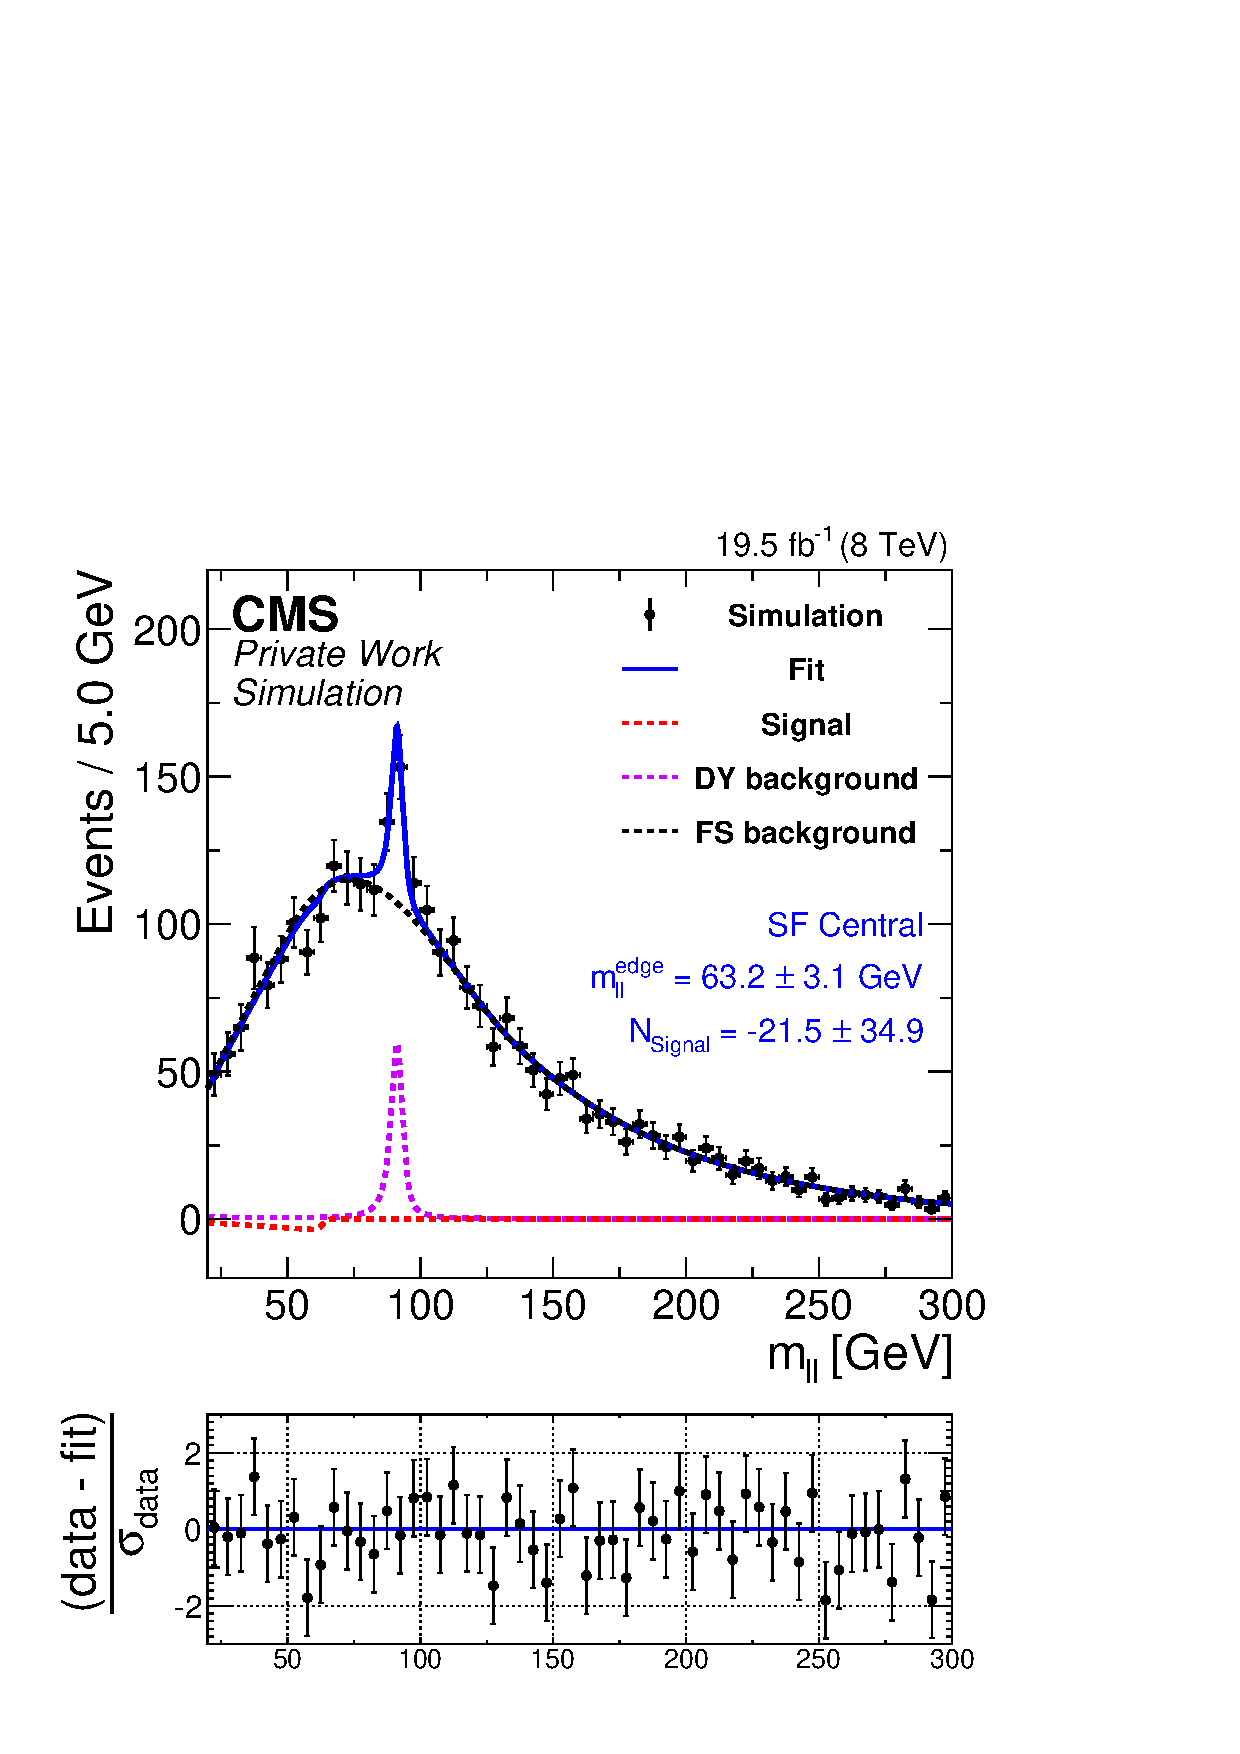
\includegraphics[width=\textwidth]{plots/results/fit/mcFits/fit2012_ETHTriangle_SignalInclusive_Combined_Full2012_ETHTriangle_MC_Central.pdf}
  \end{minipage}
  \begin{minipage}[t]{0.49\textwidth}
    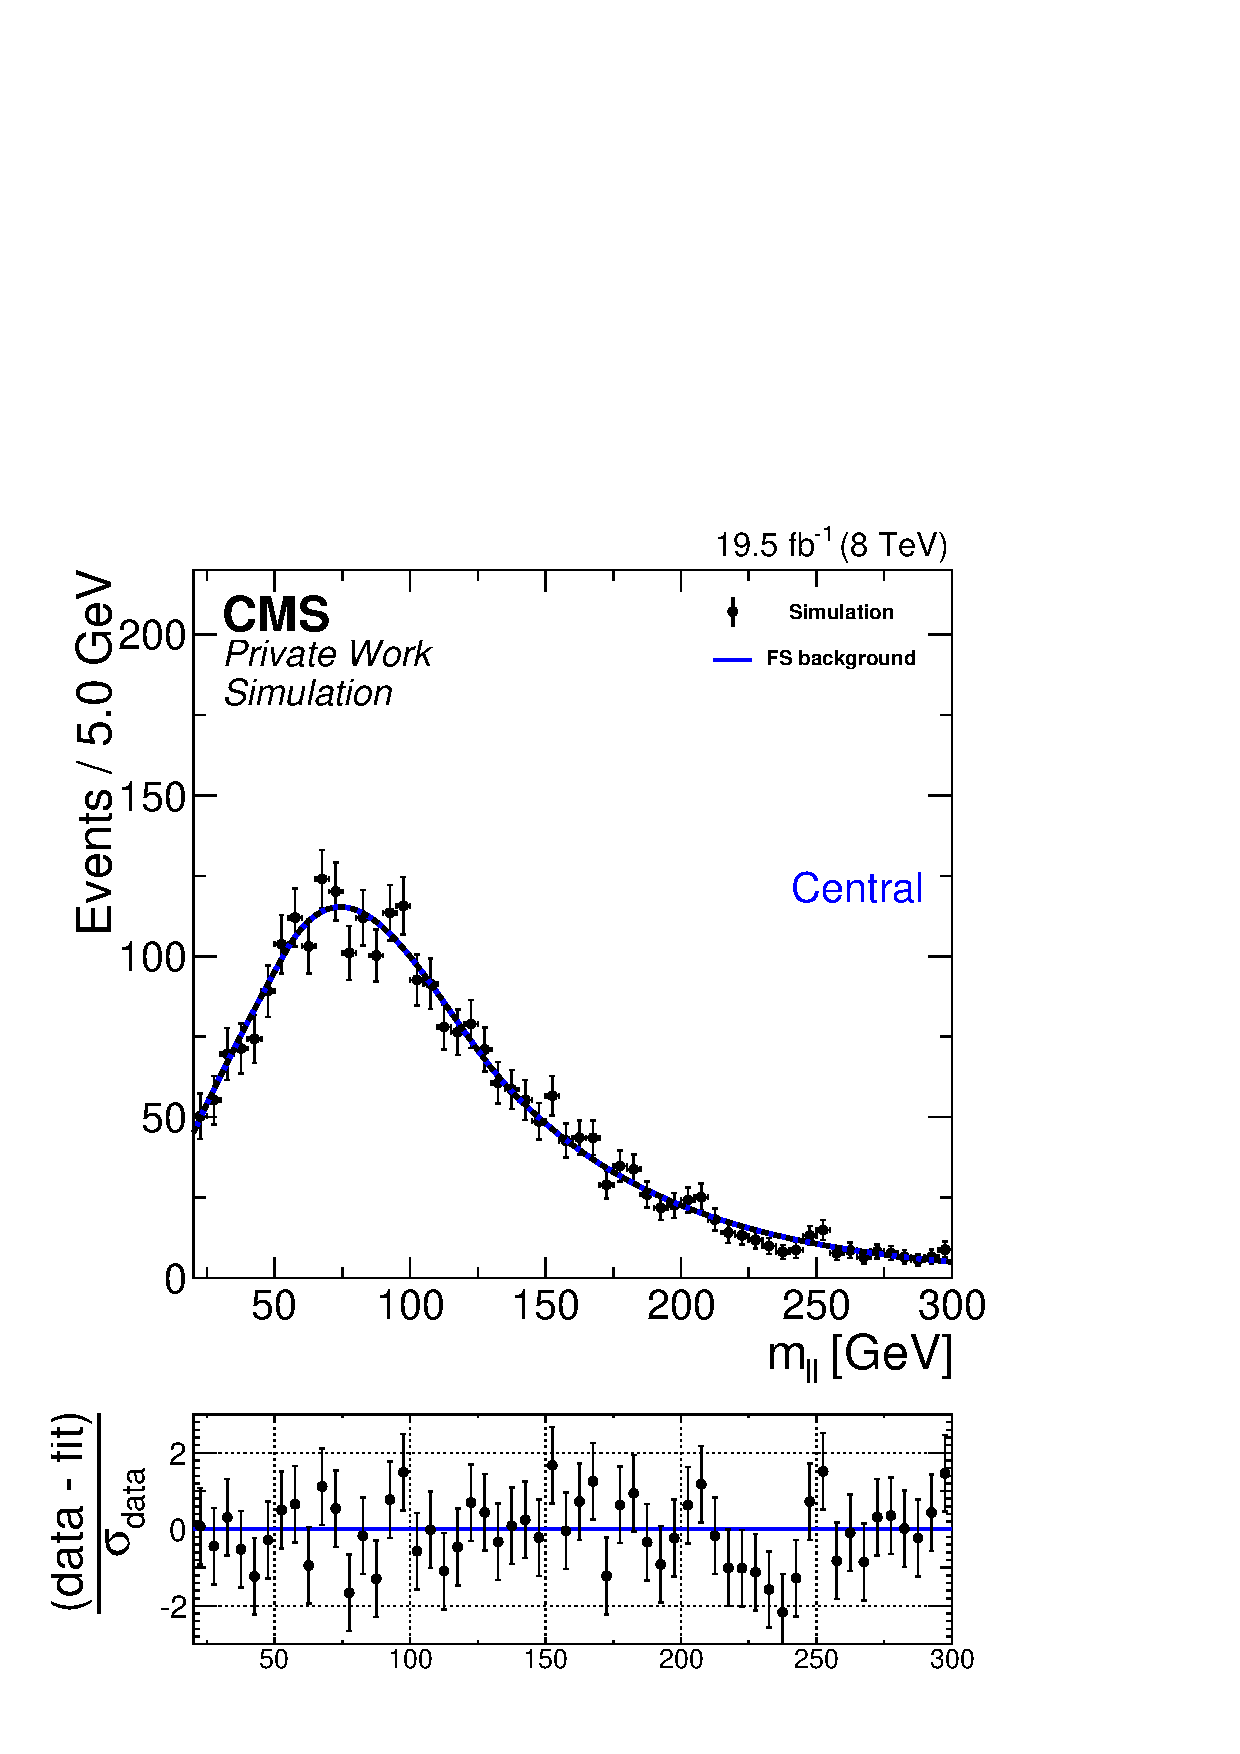
\includegraphics[width=\textwidth]{plots/results/fit/mcFits/fit2012OFOS_ETHTriangle_SignalInclusive_Combined_Full2012_ETHTriangle_MC_Central.pdf}
  \end{minipage}
  \begin{minipage}[t]{0.49\textwidth}
    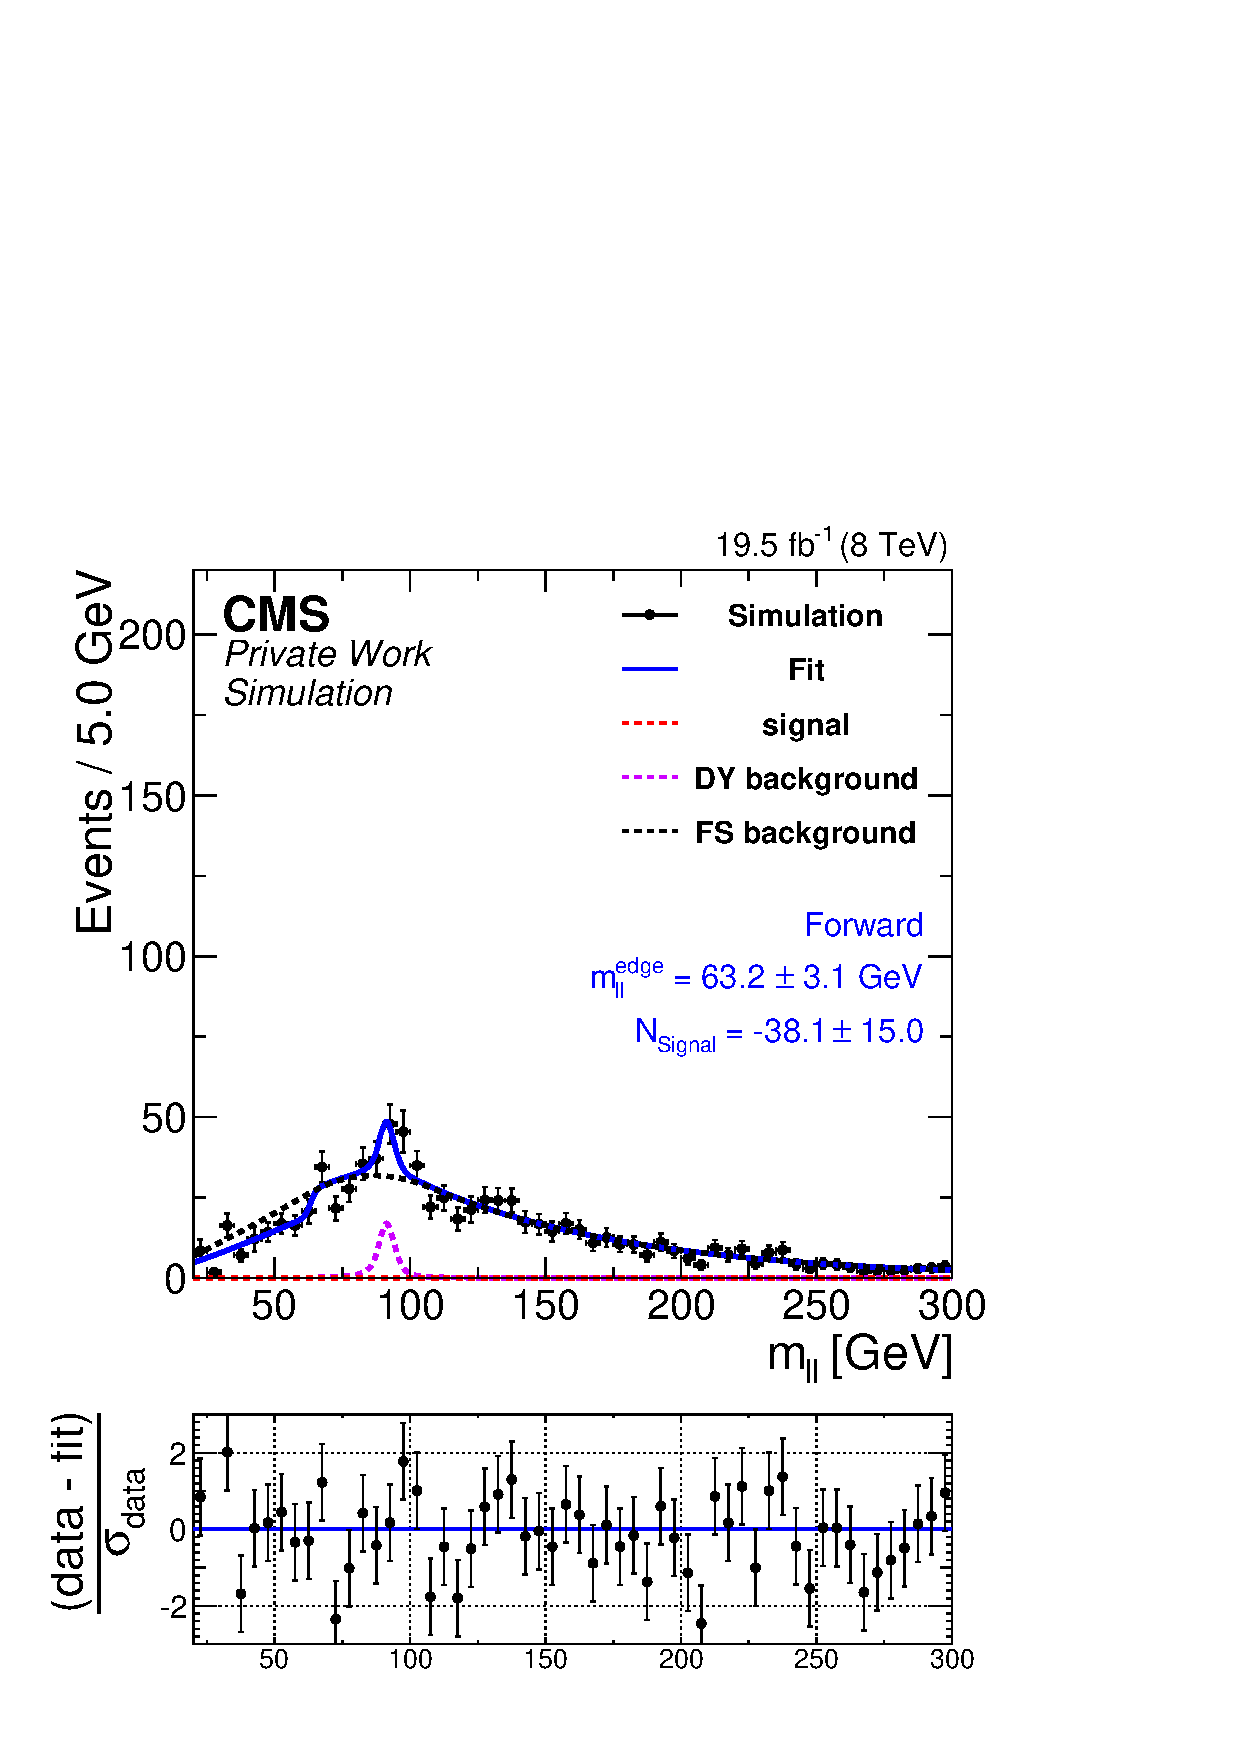
\includegraphics[width=\textwidth]{plots/results/fit/mcFits/fit2012_ETHTriangle_SignalInclusive_Combined_Full2012_ETHTriangle_MC_Forward.pdf}
  \end{minipage}
  \begin{minipage}[t]{0.49\textwidth}
    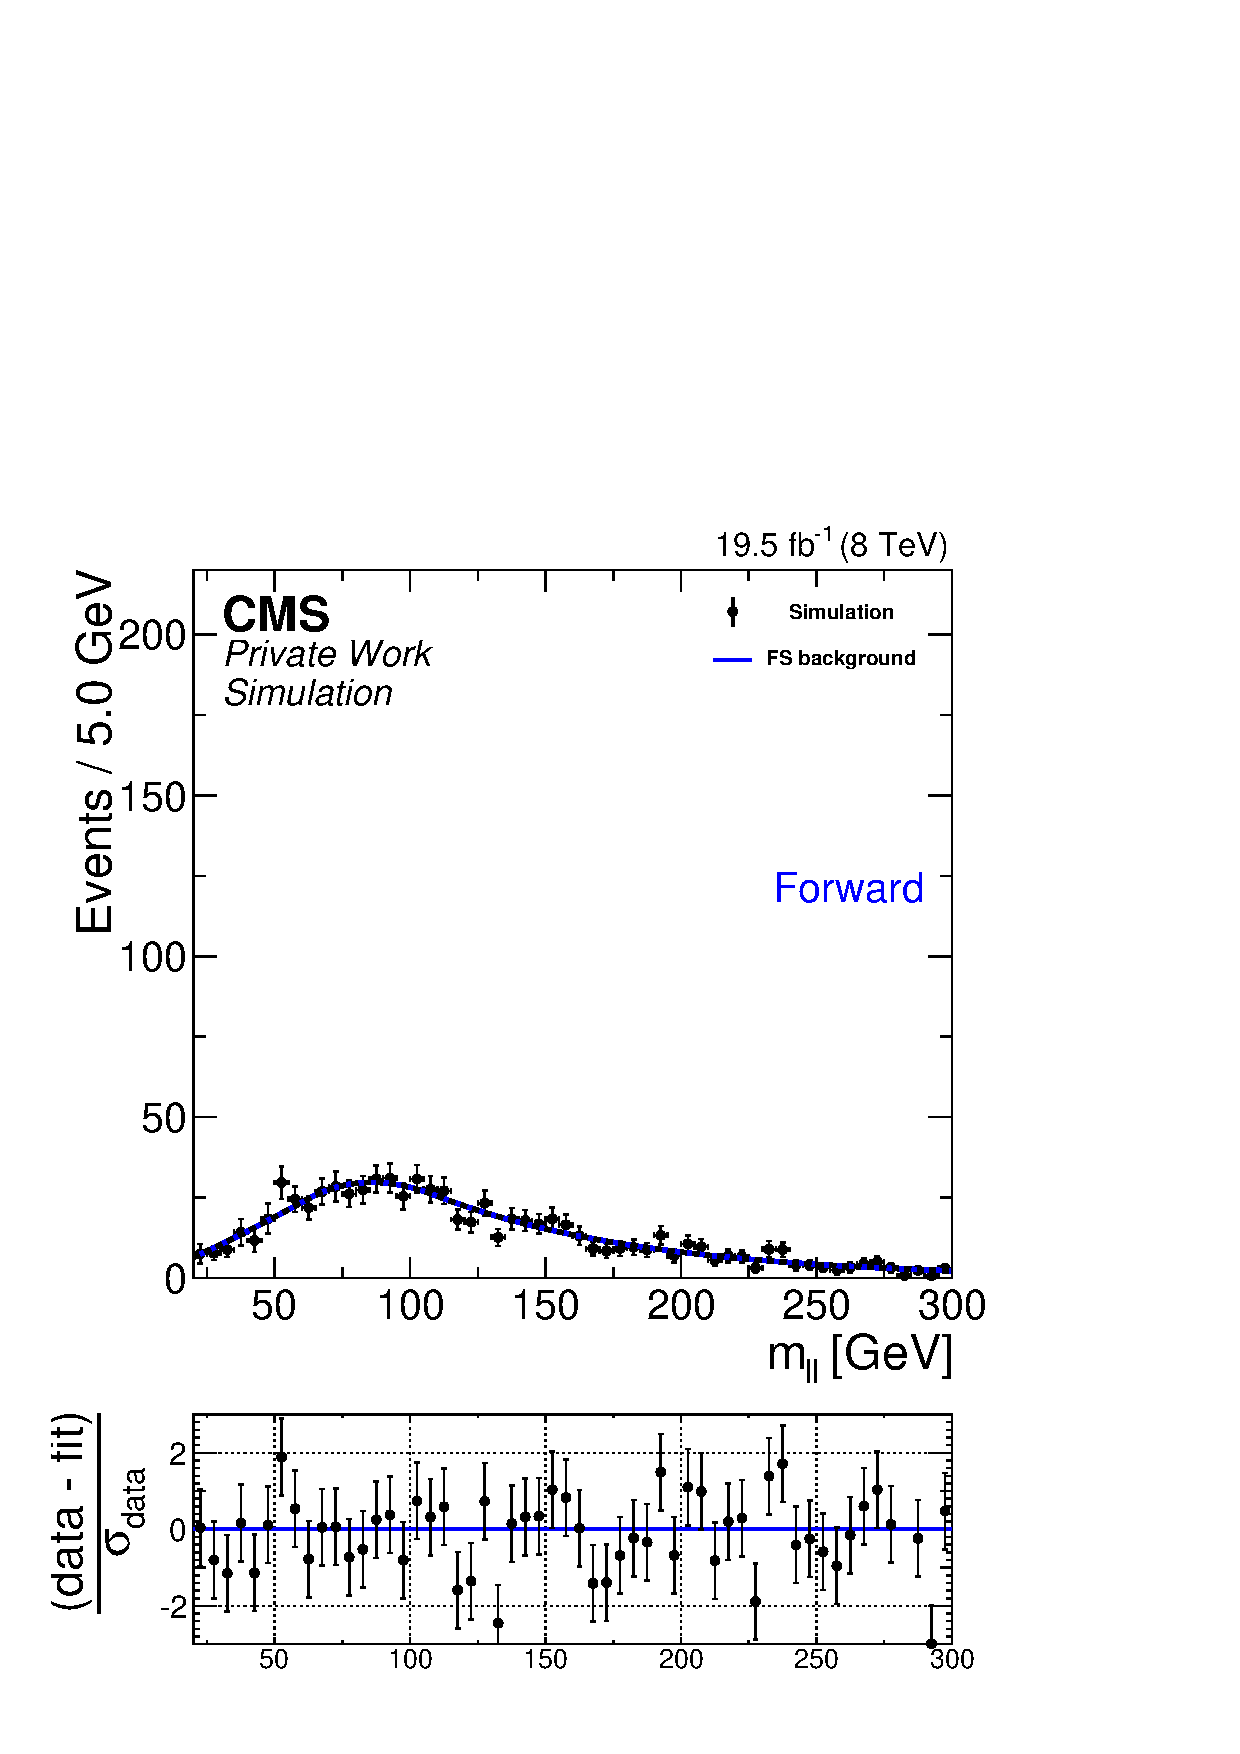
\includegraphics[width=\textwidth]{plots/results/fit/mcFits/fit2012OFOS_ETHTriangle_SignalInclusive_Combined_Full2012_ETHTriangle_MC_Forward.pdf}
  \end{minipage}
  \caption{Results for a fit to background-only simulation. Shown are the results for the SF (left) and OF (right) samples in the central (top) and forward (bottom) signal regions. The simulation is shown as black data points. The combined fit is shown as a solid blue line, while the flavour-symmetric and Z backgrounds are shown as black and violet dashed lines. The signal model is shown as a red dashed line. }
  \label{fig:mc:bgOnly}
\end{figure}

\begin{figure}[htbp]
\centering
  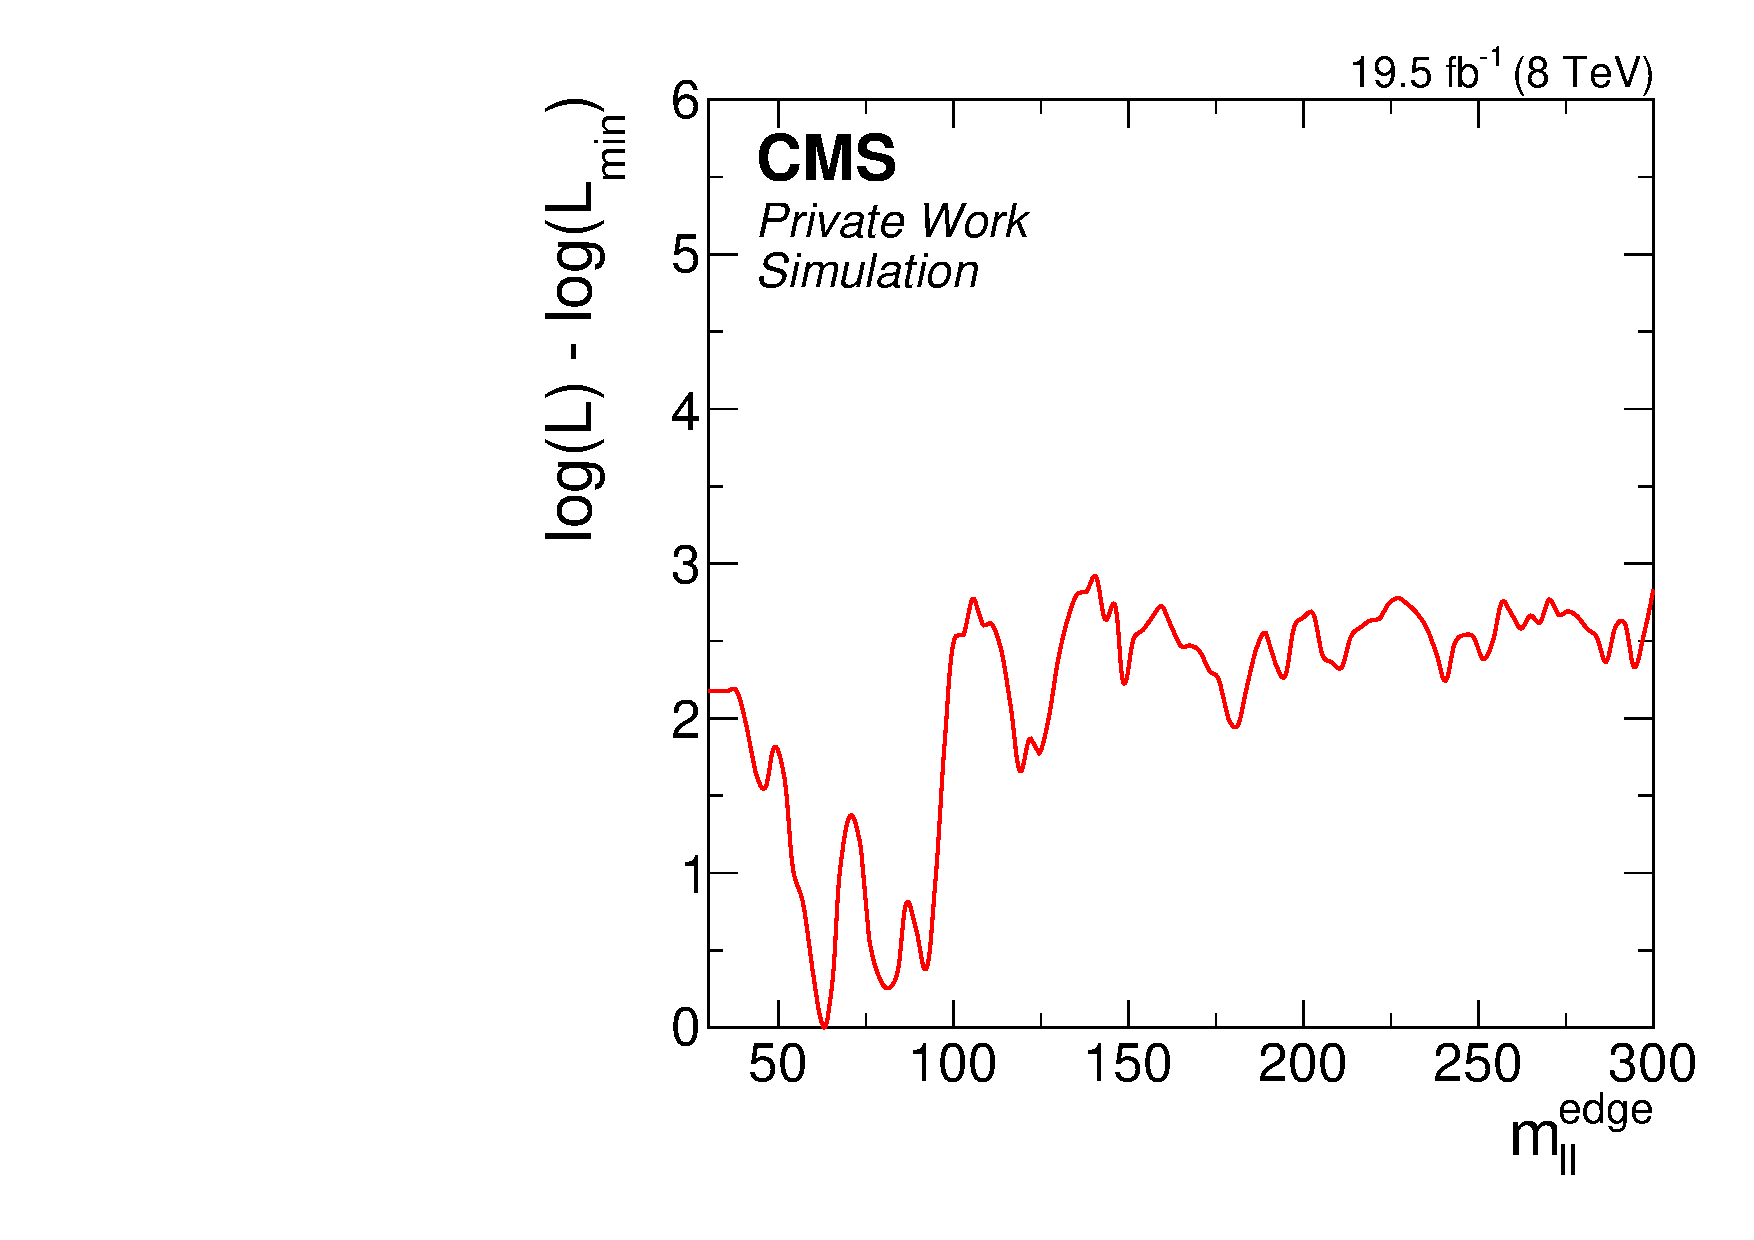
\includegraphics[width=0.6\textwidth]{plots/results/fit/mcFits/MC.pdf}
\caption{Scan of the observed log-likelihood in the signal region subtracted by the minimal value as a function of $m_{\ell\ell}^{edge}$.}
\label{fig:mc:bgOnlyProfile}
\end{figure}

The signal points S1-S4 discussed in Section~\ref{sec:sigModel} are used to test the fit's ability to reproduce the parameters of a signal. Figure~\ref{fig:mc:signalInjection} shows the results for the SF dataset in the central signal region for all four hypotheses. 

In all four cases, the correct edge position is found with good precision. In case of the fixed-edge signal point S1, the signal shape differs significantly from the triangular shape assumed in the fit. However, in the absence of background, the parameters of the signal model are reproduced with high accuracy as demonstrated in Section~\ref{sec:sigModel}. Comparing the fitted values for the number of signal events ($119.3\pm40.8$ and $122.2\pm11.1$) and \mlledge ($\unit{68.8\pm3.6}{\giga\electronvolt}$ and $\unit{68.8\pm0.6}{\giga\electronvolt}$) with and without backgrounds, the presence of the backgrounds does not significantly affect the result, except to increase the uncertainties. It can be concluded that the triangular shape is suitable to extract the signal parameters of more convex shapes. A more detailed study of the biases introduced by different signal shapes in described in Section~\ref{sec:toysW}. 

For the three slepton-edge signals S2-S4, the edge position is well reproduced by the fit. The fitted signal yield, however, can be lower than the injected one. This effect increases with \mlledge because the fit is able to accommodate higher values of \Rsfof, increasing the background contribution. This is accompanied by a slight increase of the fitted Drell--Yan yield. Another notable feature is the contribution of the signal to the flavour-symmetric backgrounds, which is of the order of 40-80 events for the studied signal points.

\begin{figure}[hbp]
  \centering
  \begin{minipage}[t]{0.49\textwidth}
    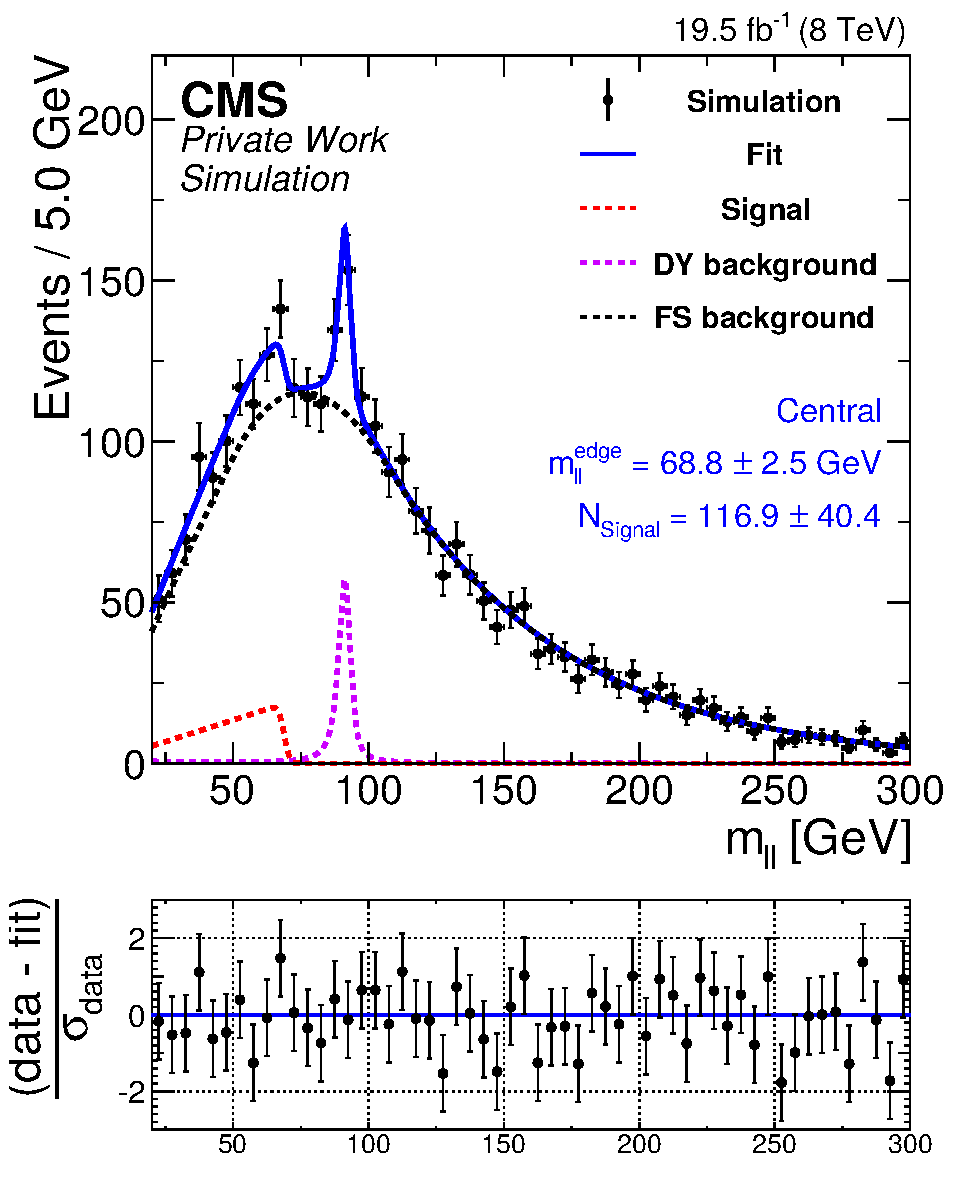
\includegraphics[width=\textwidth]{plots/results/fit/mcFits/fit2012_ETHTriangle_SignalInclusive_Combined_Full2012_ETHTriangle_MC_SignalInjected_edge_400_150_80_Central.pdf}
  \end{minipage}
  \begin{minipage}[t]{0.49\textwidth}
    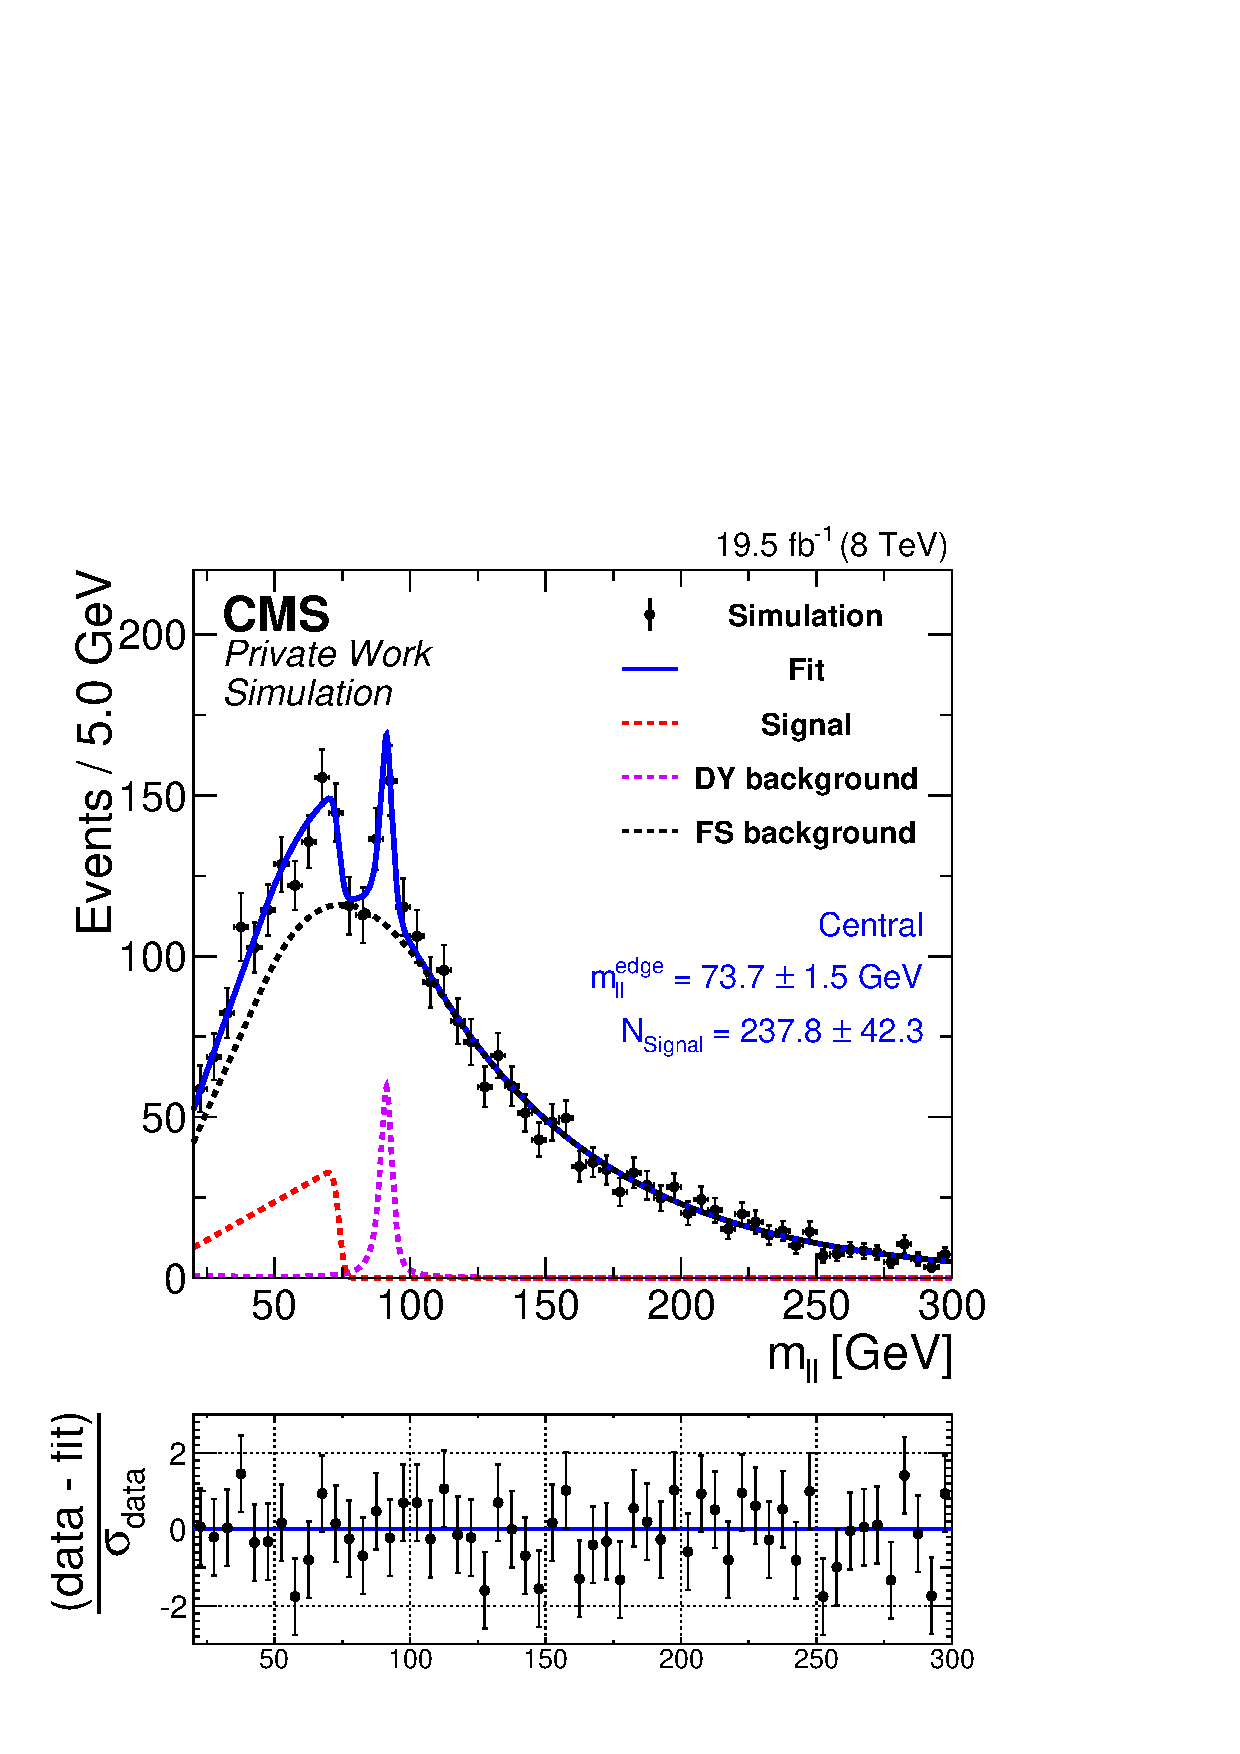
\includegraphics[width=\textwidth]{plots/results/fit/mcFits/fit2012_ETHTriangle_SignalInclusive_Combined_Full2012_ETHTriangle_MC_SignalInjected_slepton_500_175_100_Central.pdf}
  \end{minipage}
  \begin{minipage}[t]{0.49\textwidth}
    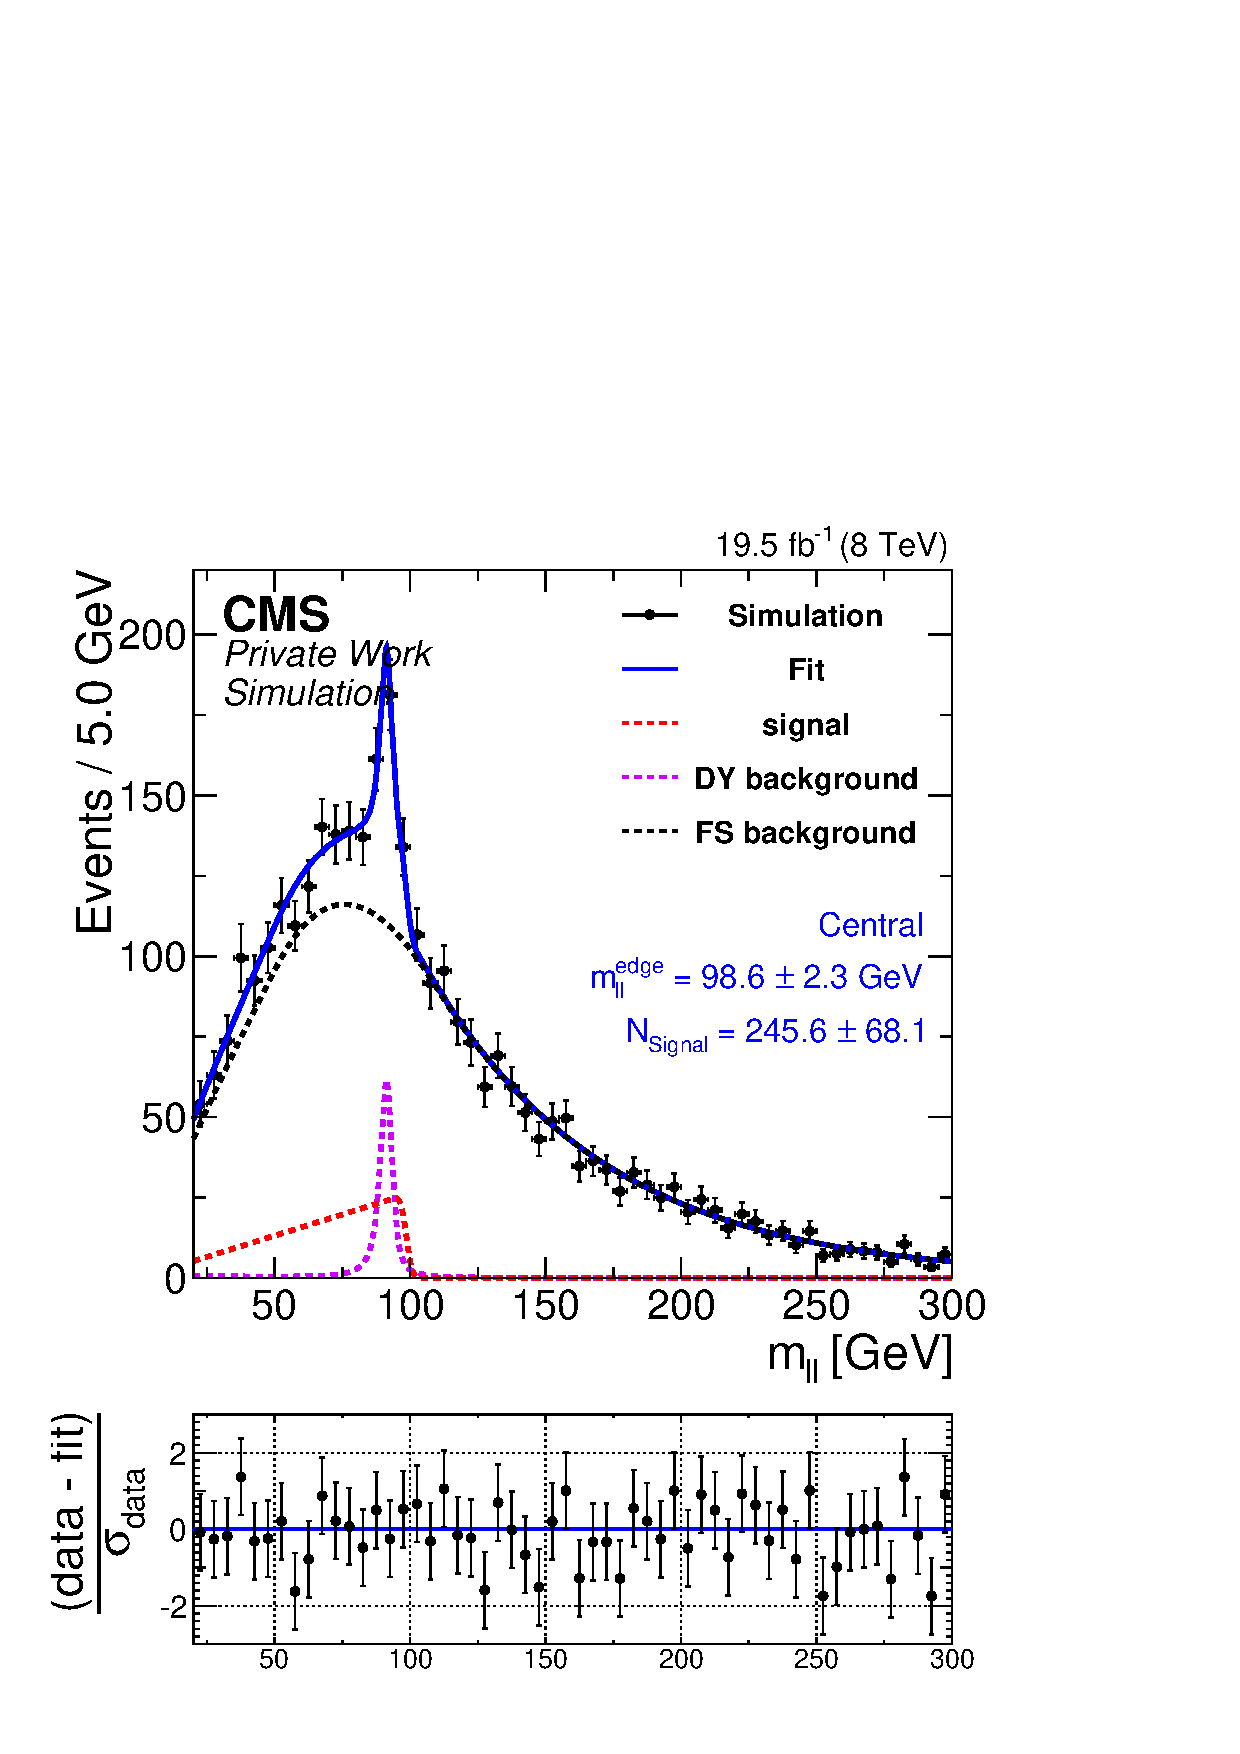
\includegraphics[width=\textwidth]{plots/results/fit/mcFits/fit2012_ETHTriangle_SignalInclusive_Combined_Full2012_ETHTriangle_MC_SignalInjected_slepton_500_200_100_Central.pdf}
  \end{minipage}
  \begin{minipage}[t]{0.49\textwidth}
    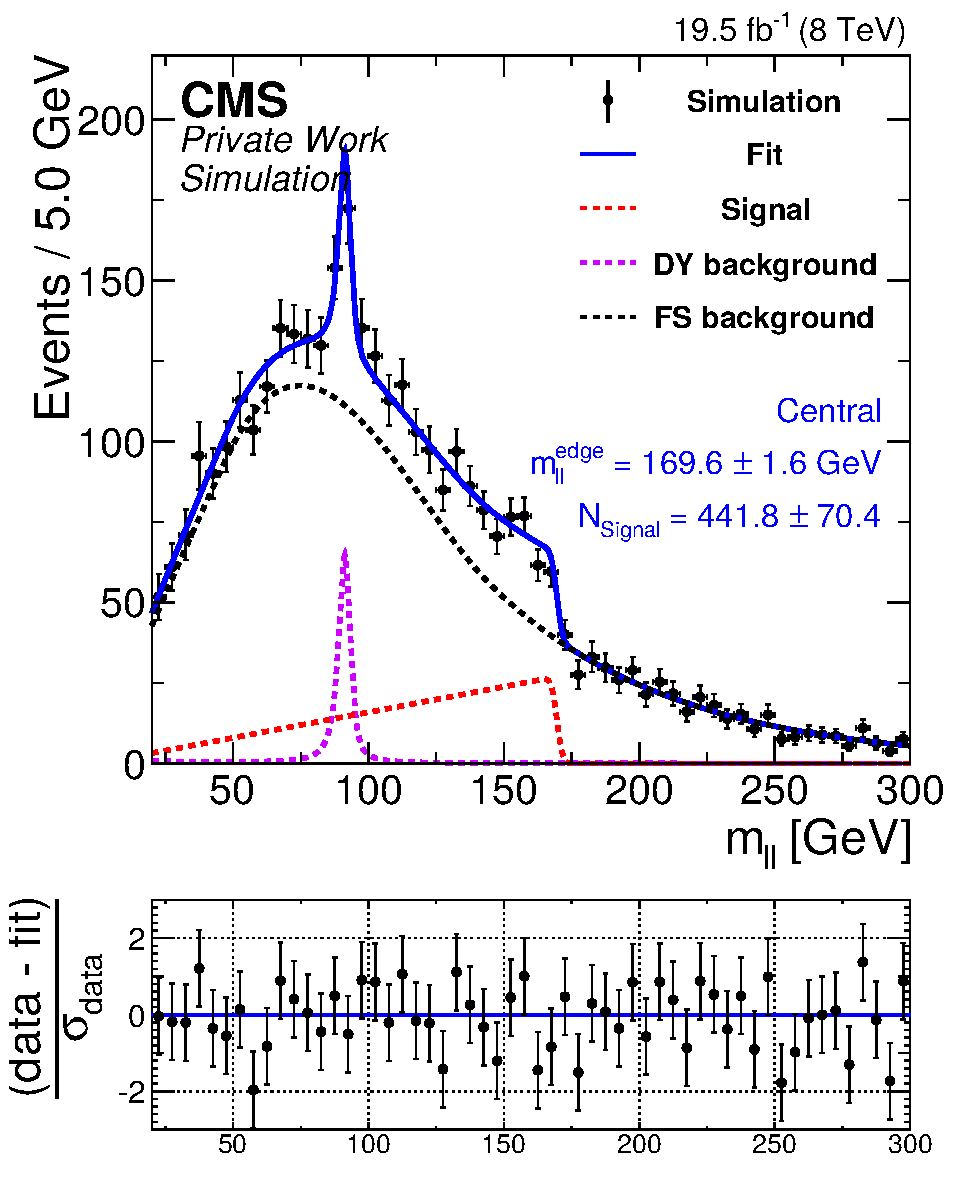
\includegraphics[width=\textwidth]{plots/results/fit/mcFits/fit2012_ETHTriangle_SignalInclusive_Combined_Full2012_ETHTriangle_MC_SignalInjected_slepton_450_275_100_Central.pdf}
  \end{minipage}
  \caption{Fit results in the central signal region for the signal point from the fixed-edge model S1 (top left) and the three points from the slepton-edge model S2 (top right), S3 (bottom left), and S4 (bottom right). The combined fit is shown as a solid blue line, while the flavour-symmetric and Z backgrounds are shown as black and violet dashed lines. The signal model is shown as a red dashed line.}
  \label{fig:mc:signalInjection}
\end{figure}




\subsection{Fit performance studies using toy datasets}
\label{sec:toys}
The performance of the fit is furthermore studied using toy datasets. These are generated by fitting the background shape for flavour-symmetric backgrounds to OF events in simulation. From this shape new opposite-flavour datasets are generated, fluctuating the normalisation using a Poisson distribution. Electron-electron and muon-muon datasets are generated from the sum of the  shape for flavour-symmetric backgrounds and the Drell--Yan model. The normalisation of this shape is given by the normalisation for flavour-symmetric backgrounds multiplied by \Rsfof plus the combined JZB and \MET-template predictions. This yield is split into the \EE and \MM datasets according to the measured \Reeof and \Rmmof values. Each of the two yields is fluctuated independently according to a Poisson distribution when dicing the toy datasets. If desired, a signal can be injected in the same-flavour datasets using the nominal signal shape in a similar fashion. To reflect that the signal yield is expected to be higher in the central dilepton selection, the signal contribution in the forward selection is chosen to be smaller by a factor of three. The combined fit is performed on each of the datasets generated in this fashion. As the nominal background shape evaluation is very resource intensive, the parametrisation from the 2011 analysis (see Equation~\ref{eq:2011}) is used in these studies in order to generate sufficient statistics, after verifying that this has no significant impact on the results. In general about 1000 toy datasets are generated for each of the configurations described below.
\subsubsection{Studies without signal injection}
\label{sec:toysWO}
The edge fit is performed on toys generated from the background models. In one case, the toys are fitted with a floating edge position. In the other, the edge is fixed at $\unit{70}{\giga\electronvolt}$. Figure~\ref{fig:toys:backgroundOnly} shows the resulting distributions. On the left side, the number of fitted signal events in the central region divided by its uncertainty is shown. In the case of a fixed edge the fit results are distributed following a unit-Gaussian centred around zero, as expected in absence of a signal.  For the case of a floating edge position, however, the distribution exhibits two peaks, symmetrically below and above zero. This is a manifestation of the ``look-elsewhere-effect'' introduced by the degree of freedom of the edge position, which allows the fit to find a value of \mlledge where introducing a positive or negative signal improves the likelihood value because of the statistical fluctuations of the dataset. As this may result in lower values of the negative log-likelihood compared to the case of the fixed edge, a bias is introduced towards edge positions where a signal component can be accommodated.

On the right side of Figure~\ref{fig:toys:backgroundOnly}, the distributions of the fitted values of \Rsfof are shown, again for the central selection. In both cases, the value used in the generation of the toys of 1.013 is well reproduced. Also, the width of the distribution is identical in both cases,  illustrating that the floating edge position does not introduce biases apart from favouring edge positions where the fluctuations of the dataset allow for a signal component, as discussed above.
\begin{figure}[h]
  \centering
  \begin{minipage}[t]{0.49\textwidth}
    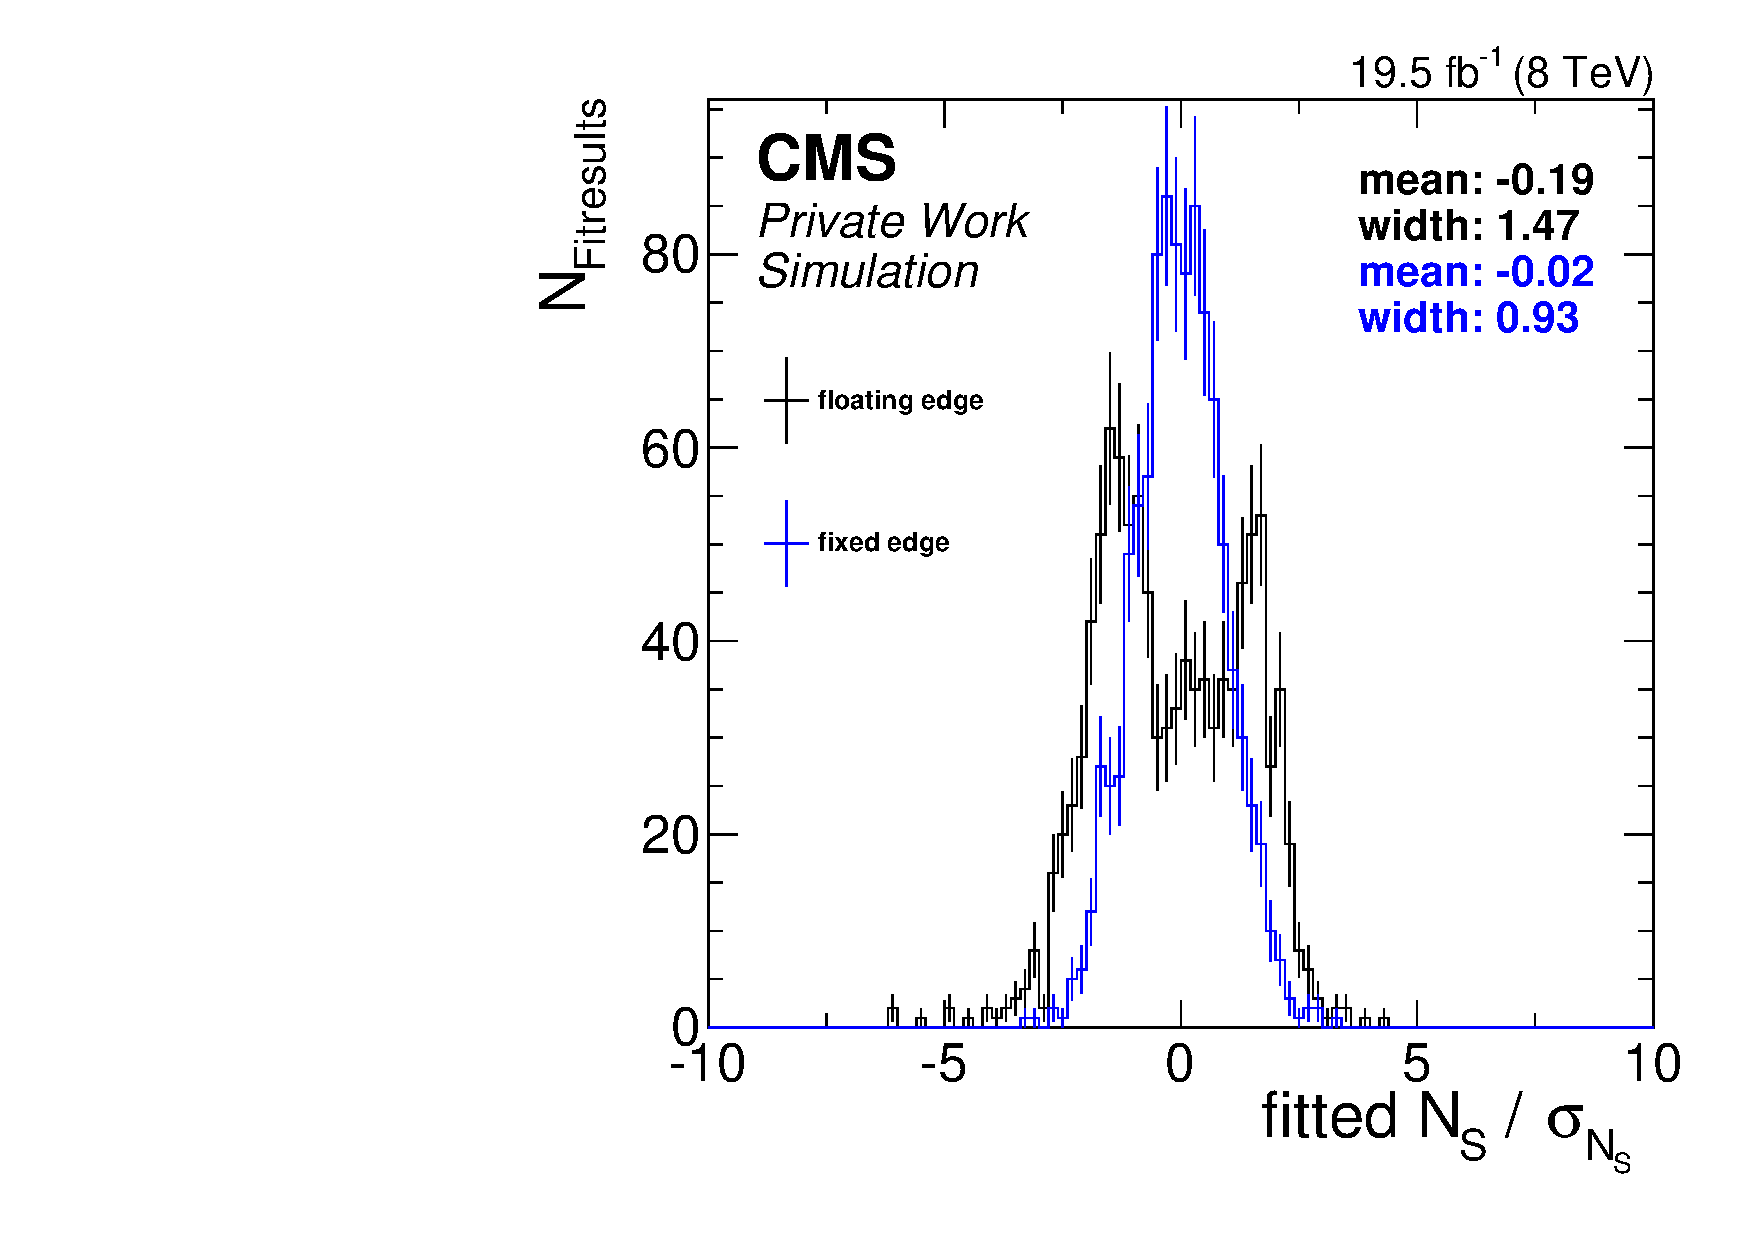
\includegraphics[width=\textwidth]{plots/results/fit/toyResults/nS_floatVsFixed.pdf}
  \end{minipage}
  \begin{minipage}[t]{0.49\textwidth}
    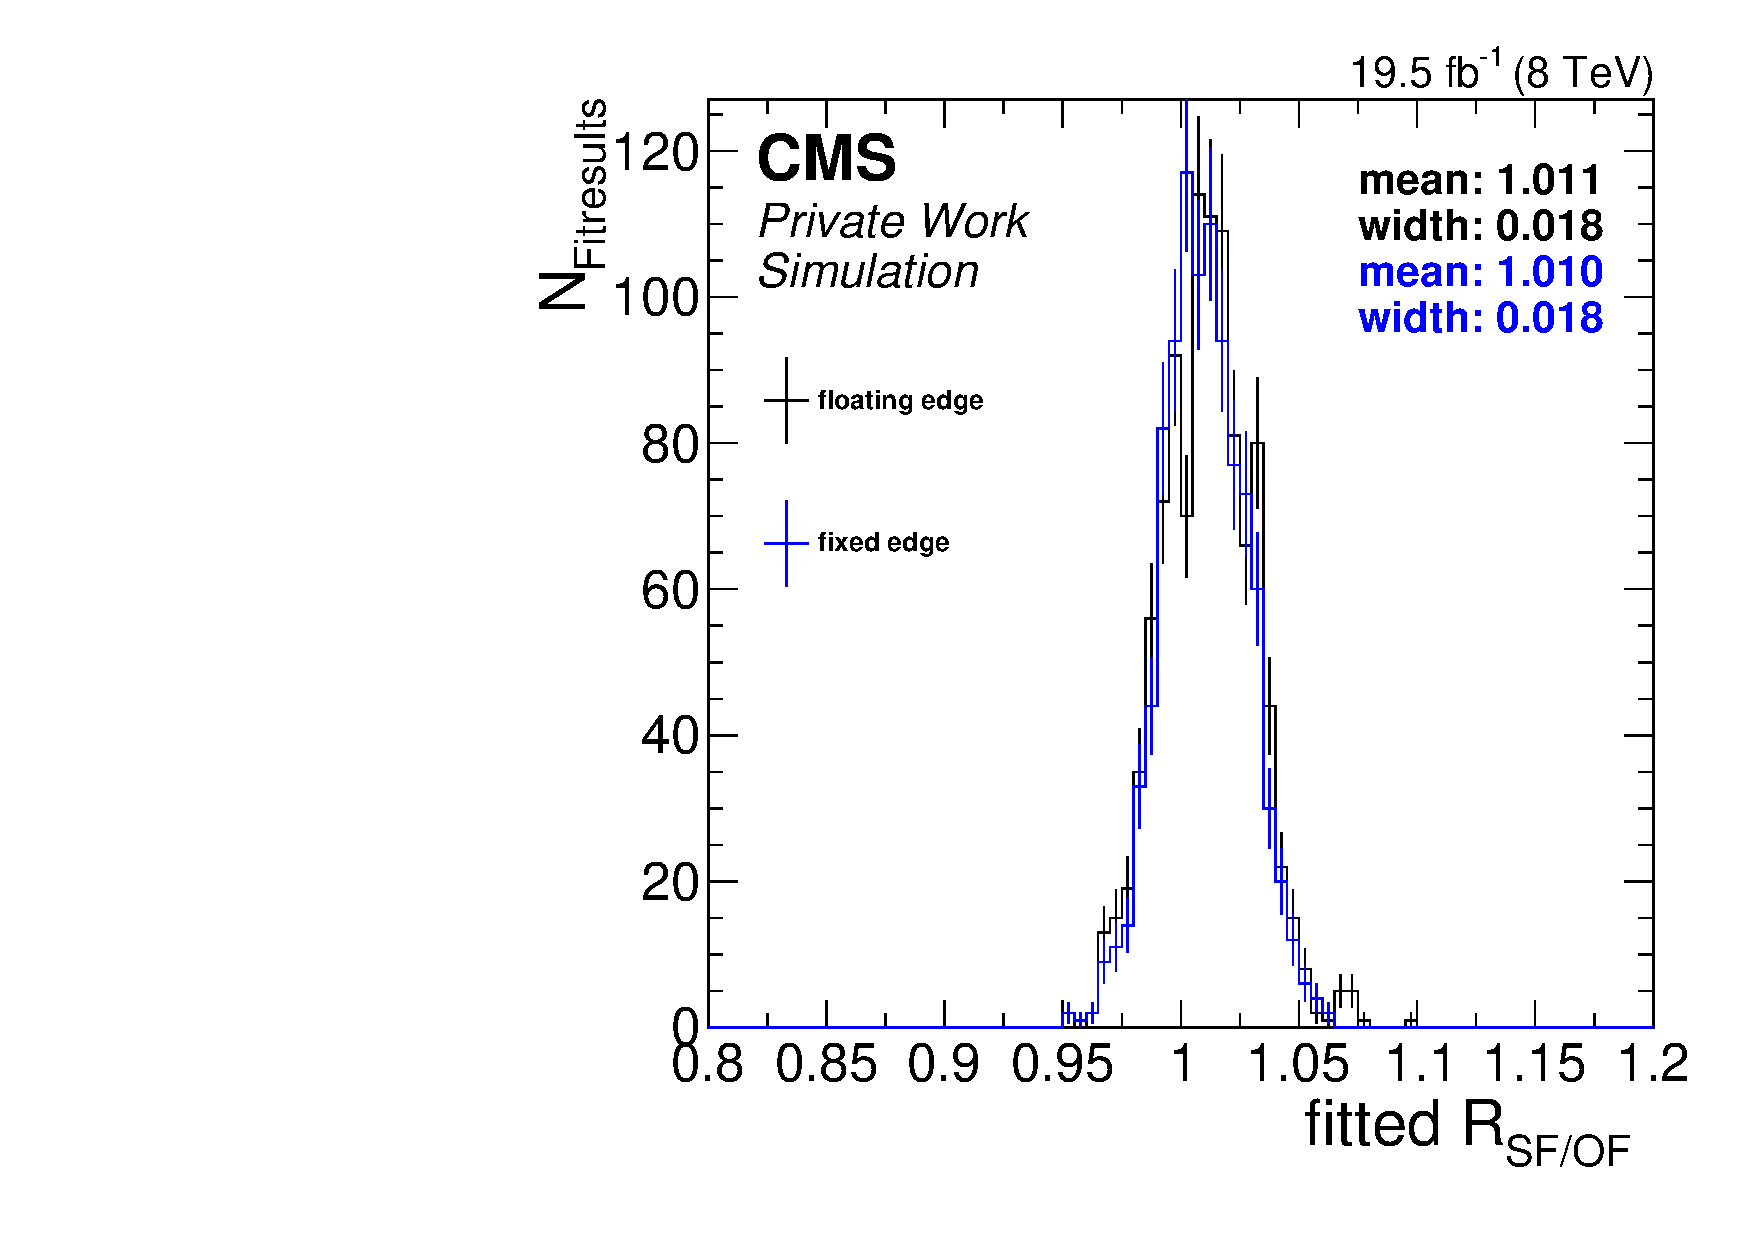
\includegraphics[width=\textwidth]{plots/results/fit/toyResults/rSFOF_floatVsFixed.pdf}
  \end{minipage}

  \caption{Distribution of fit observables in toy studies for a background only scenario. Shown are the fitted number of signal events divided by their uncertainty in the central region (left) and the corresponding fitted values of \Rsfof (right). The results for a floating edge are shown in black and those for a fixed edge position in blue.}
  \label{fig:toys:backgroundOnly}
\end{figure}

The distribution of the fitted edge position versus the initial value is shown in Figure~\ref{fig:toys:backgroundOnlyFloatEdge}. The initial values has been randomised between 0 and $\unit{300}{\giga\electronvolt}$. To ensure that the initial value is inside the allowed range for \mlledge and not too close to the lower boundary, diced values below $\unit{35}{\giga\electronvolt}$ are rejected. In absence of a signal a strong correlation between the initial and observed value of \mlledge is observed. This suggests that the fit tends to converge at the next local minimum of the negative log-likelihood. It is therefore necessary to choose a suitable initial value close to the global minimum and validate the results with a scan of the log-likelihood, as shown in Figure~\ref{fig:mc:bgOnlyProfile}. 

\begin{figure}[htbp]
  \centering

    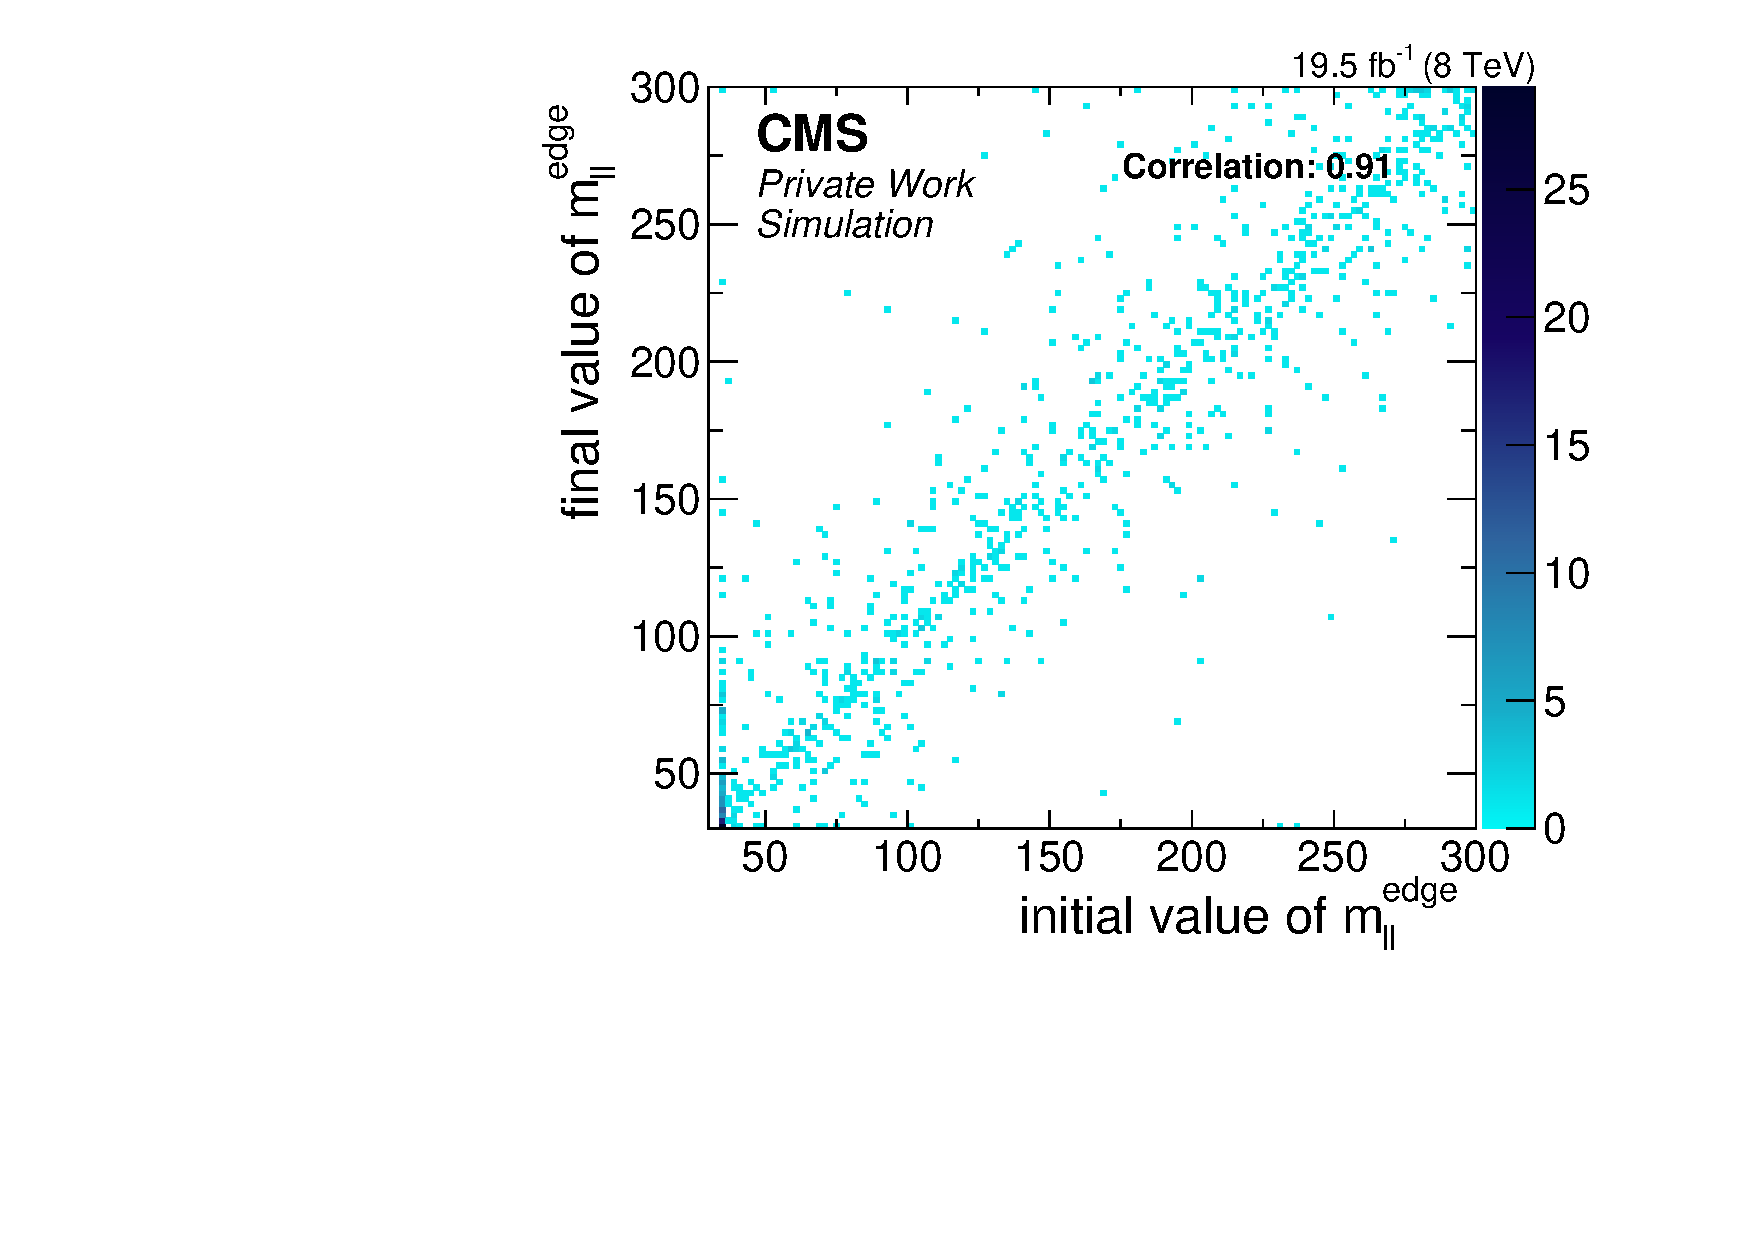
\includegraphics[width=0.6\textwidth]{plots/results/fit/toyResults/fittedM0vsinitialM0_backgroundOnly_randM0_NegSig.pdf}
  \caption{Distribution of fitted versus initial values of \mlledge in the case of the randomised initial values for toys without an injected signal.}
  \label{fig:toys:backgroundOnlyFloatEdge}
\end{figure}

As an additional check, toys are generated with \Rsfof shifted by $\pm1\sigma$ from its nominal value. These toys are afterwards fitted with \Rsfof constrained to the nominal value and the results are shown in Figure~\ref{fig:toys:systShift}. The same distributions are shown as above. For the signal yield divided by its uncertainty, the double peak structure observed in the nominal configuration changes to a single peak that is shifted to negative signal yields for the toys generated with lower and to positive signal yields for those generated with higher values of \Rsfof. This is caused by the fact that \Rsfof is constrained to the nominal value in the fit. For the fitted values of \Rsfof, the width of the distribution is unchanged, but the systematic shifts in the generation of the toys is reflected in their means. The fit is therefore able to correct for systematic biases in \Rsfof. However, the observed shifts of the mean (0.025 and -0.023) are smaller than those introduced in the generation of the toys ($\pm0.037$, the uncertainty of \Rsfof), suggesting that part of the systematic shift is absorbed by the fit by introducing a signal contribution. Still, this is a significant improvement over the counting experiment approach, where no such correction is possible.  
\begin{figure}[thbp]
  \centering
  \begin{minipage}[t]{0.49\textwidth}
    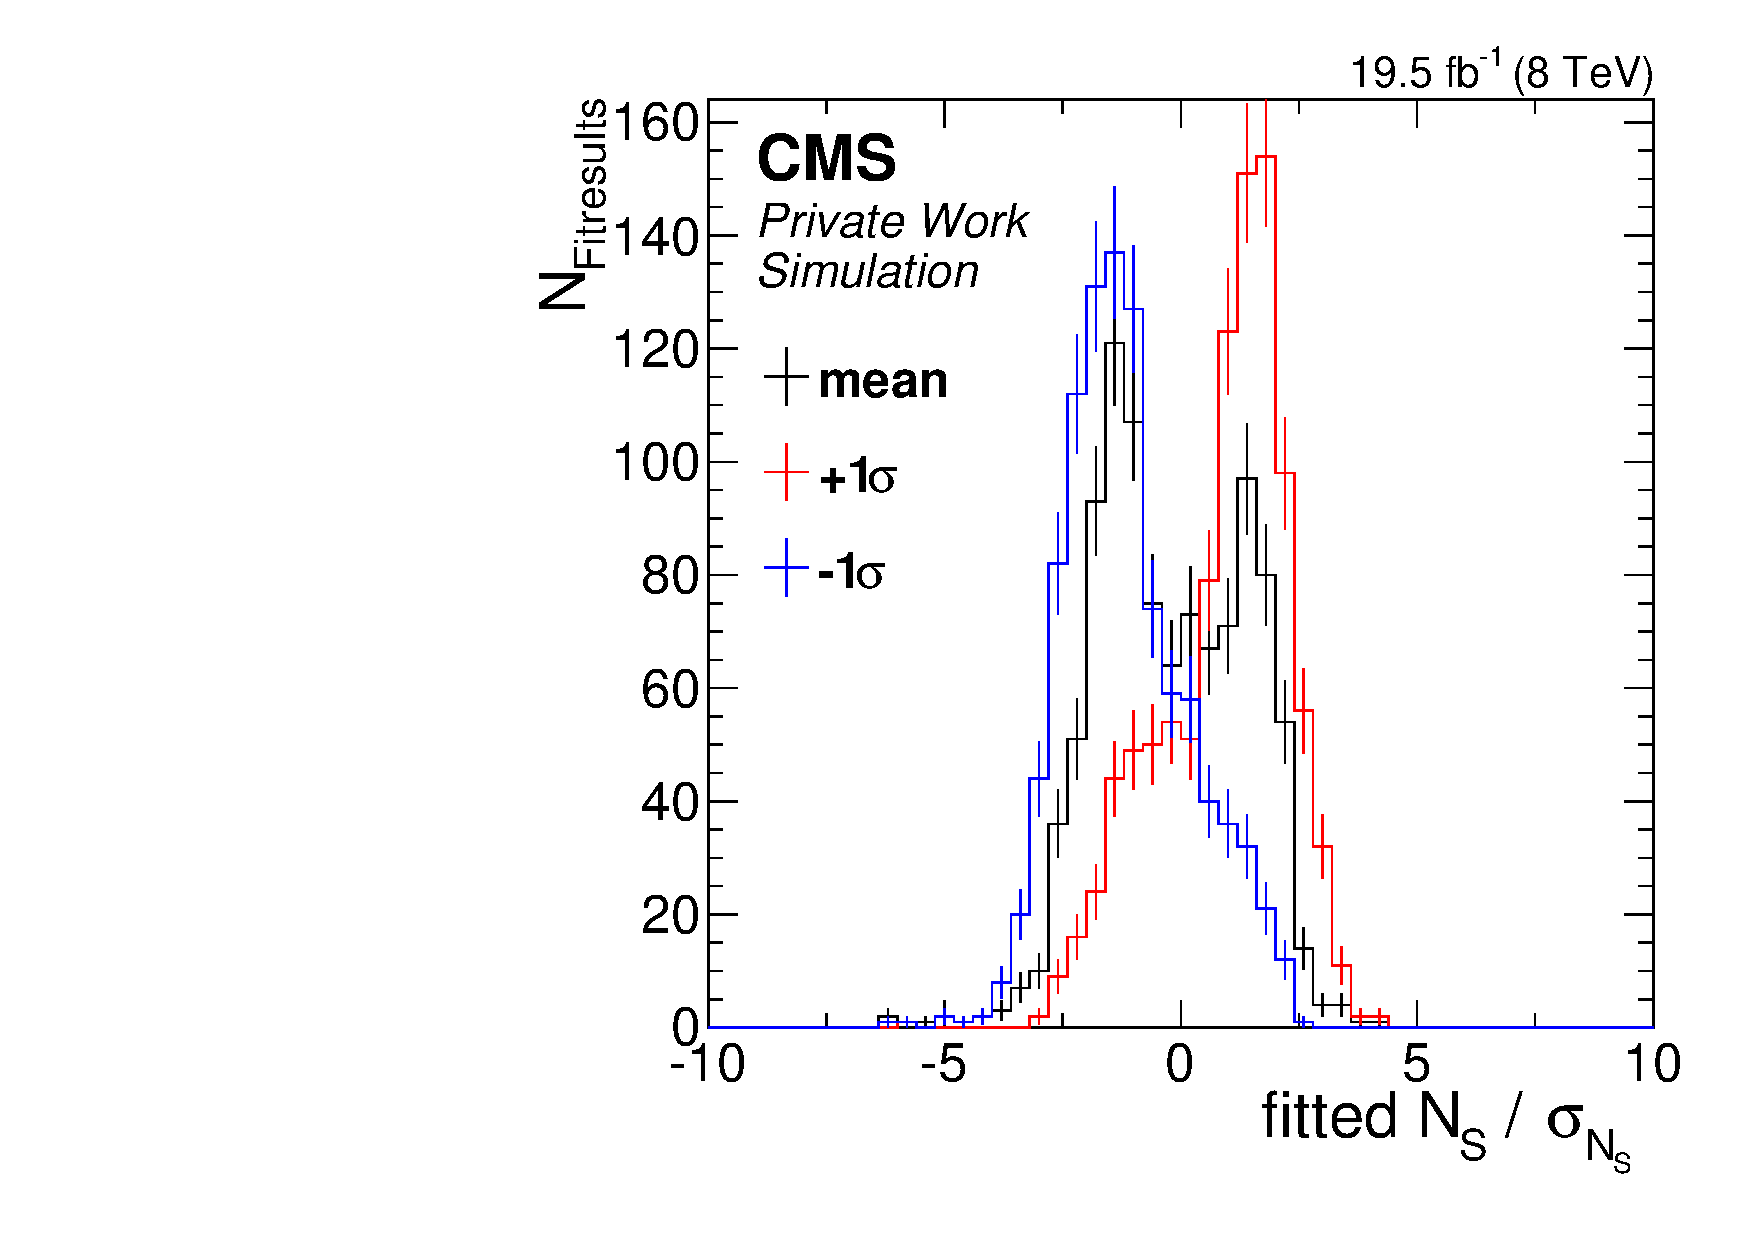
\includegraphics[width=\textwidth]{plots/results/fit/toyResults/nS_systShift.pdf}
  \end{minipage}
  \begin{minipage}[t]{0.49\textwidth}
    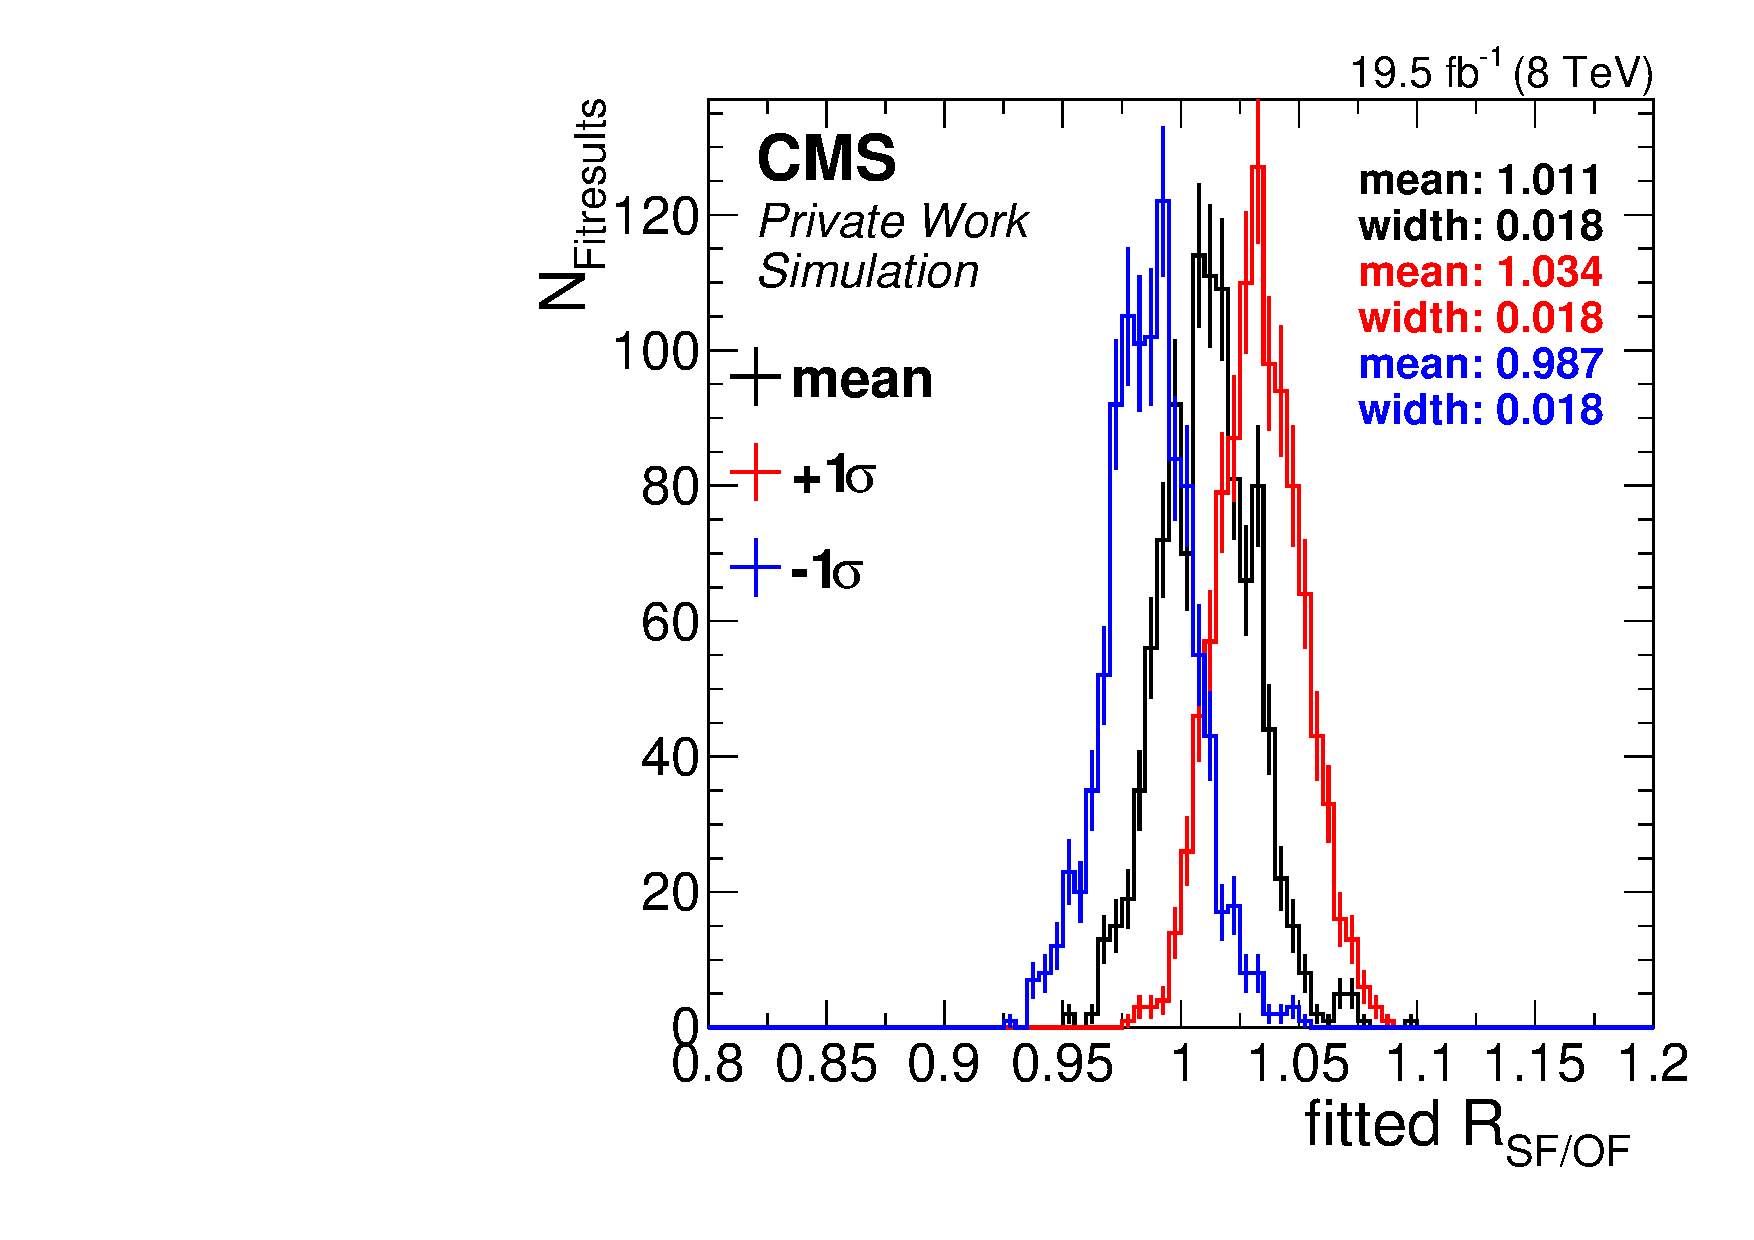
\includegraphics[width=\textwidth]{plots/results/fit/toyResults/rSFOF_systShift.pdf}
  \end{minipage}

  \caption{Distribution of fit observables in toy studies for background only toys with and without systematically shifted \Rsfof in the generation of the toys. Shown are the fitted number of signal events divided by its uncertainty in the central region (left) and the fitted value of \Rsfof (right) in the signal region.}
  \label{fig:toys:systShift}
\end{figure}
\subsubsection{Toy studies with signal injection}
\label{sec:toysW}
The fit performance in the presence of a signal is tested by injection of a signal of 125 events with an edge position of 70 GeV in the central region and a third of that number in the forward region. As for the backgrounds, the signal yields is fluctuated according to a Poisson distribution in the generation of the toys. Figure \ref{fig:toys:signalInjected} shows the resulting distribution of fit results for a selection of observables in the central signal region. The distribution of the number of signal events is well described by a Gaussian with a mean of about 124 events, very close to the injected number, and a width of 41 events. Divided by the fitted uncertainty, this gives a unit-Gaussian with a mean of about 2.9. The edge position is also Gaussian distributed, with a mean of about $\unit{70}{\giga\electronvolt}$, also reproducing the injected value very well, and a width of about $\unit{1.8}{\giga\electronvolt}$. Comparing the distribution of \Rsfof with that in Figure~\ref{fig:toys:backgroundOnly}, it shows that the presence of a signal does not bias the result towards higher values. 

\begin{figure}[hbp]
  \centering
  \begin{minipage}[t]{0.49\textwidth}
    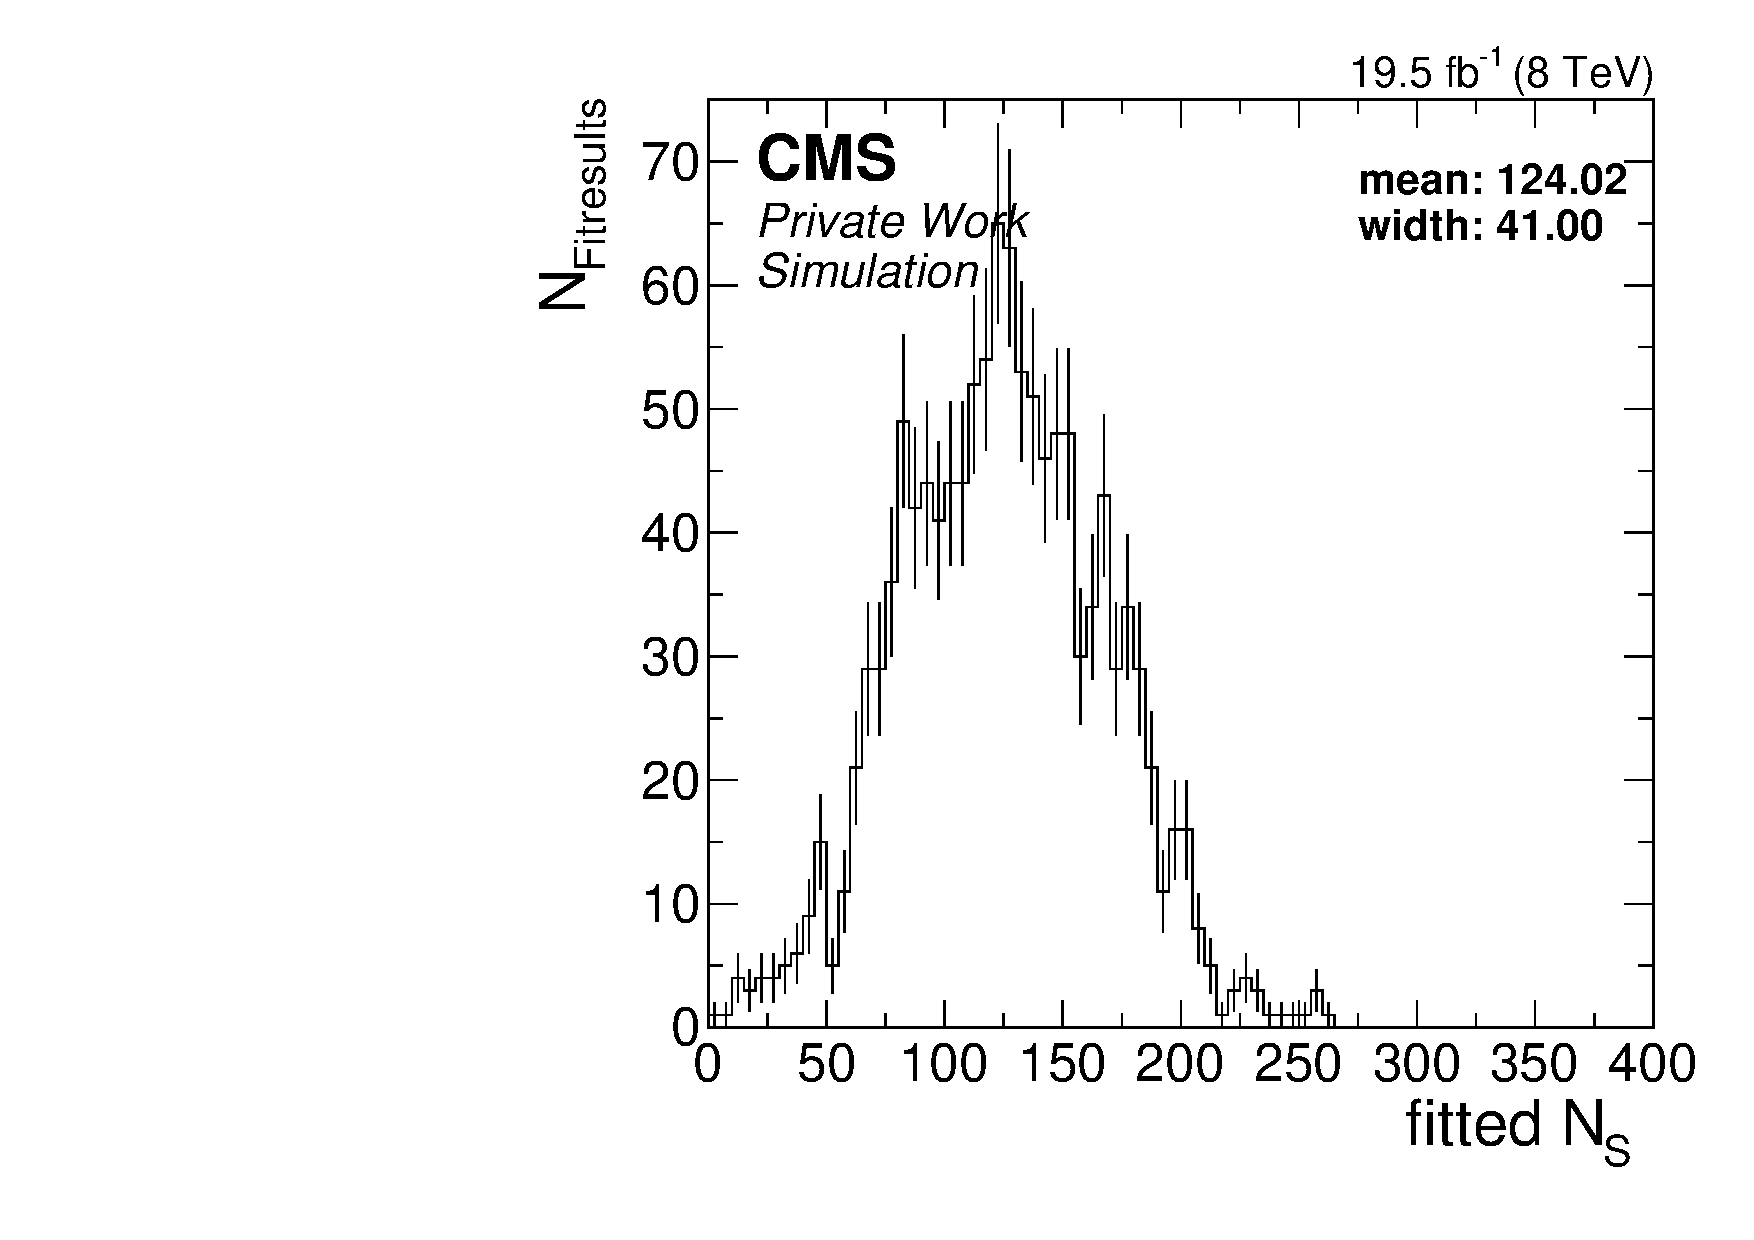
\includegraphics[width=\textwidth]{plots/results/fit/toyResults/nSPure_signalInjected.pdf}
  \end{minipage}
  \begin{minipage}[t]{0.49\textwidth}
    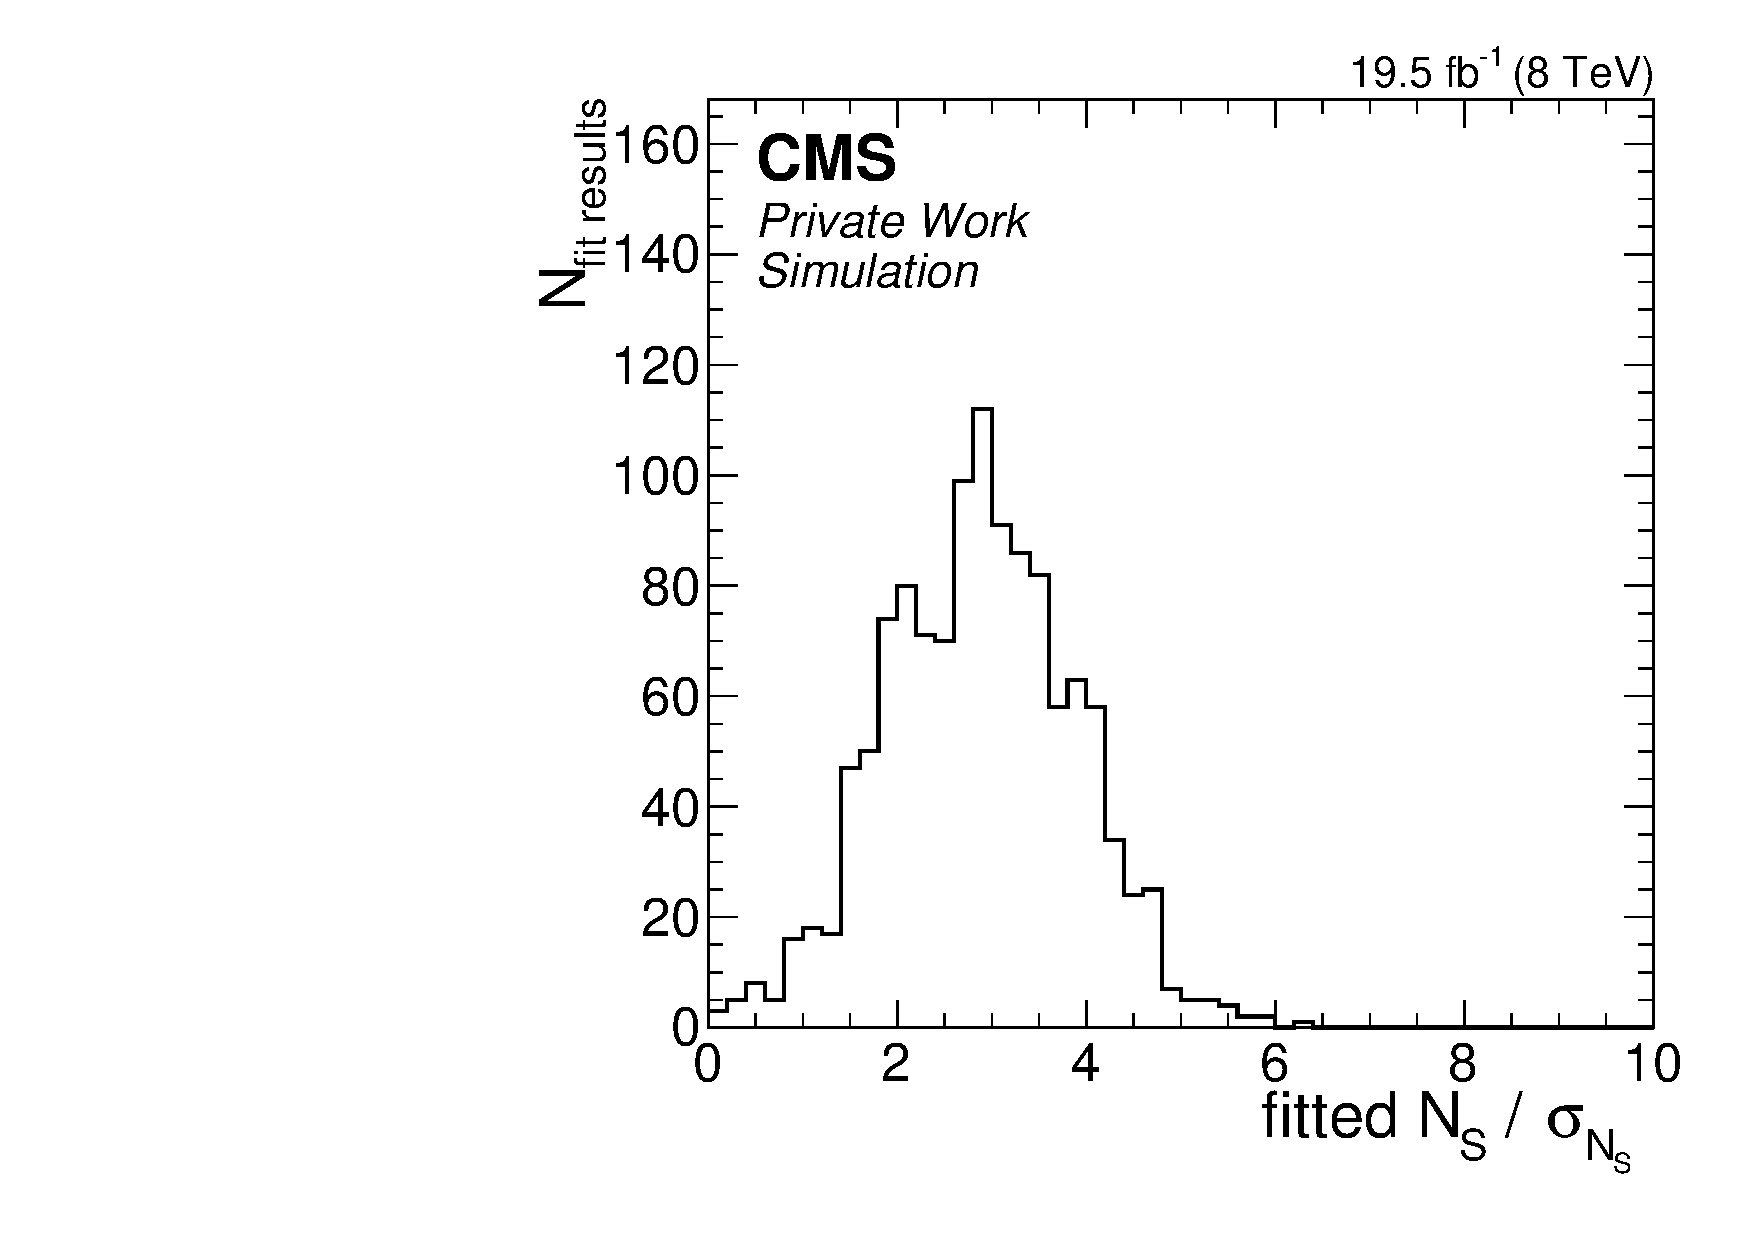
\includegraphics[width=\textwidth]{plots/results/fit/toyResults/nS_signalInjected.pdf}
  \end{minipage}
  \begin{minipage}[t]{0.49\textwidth}
    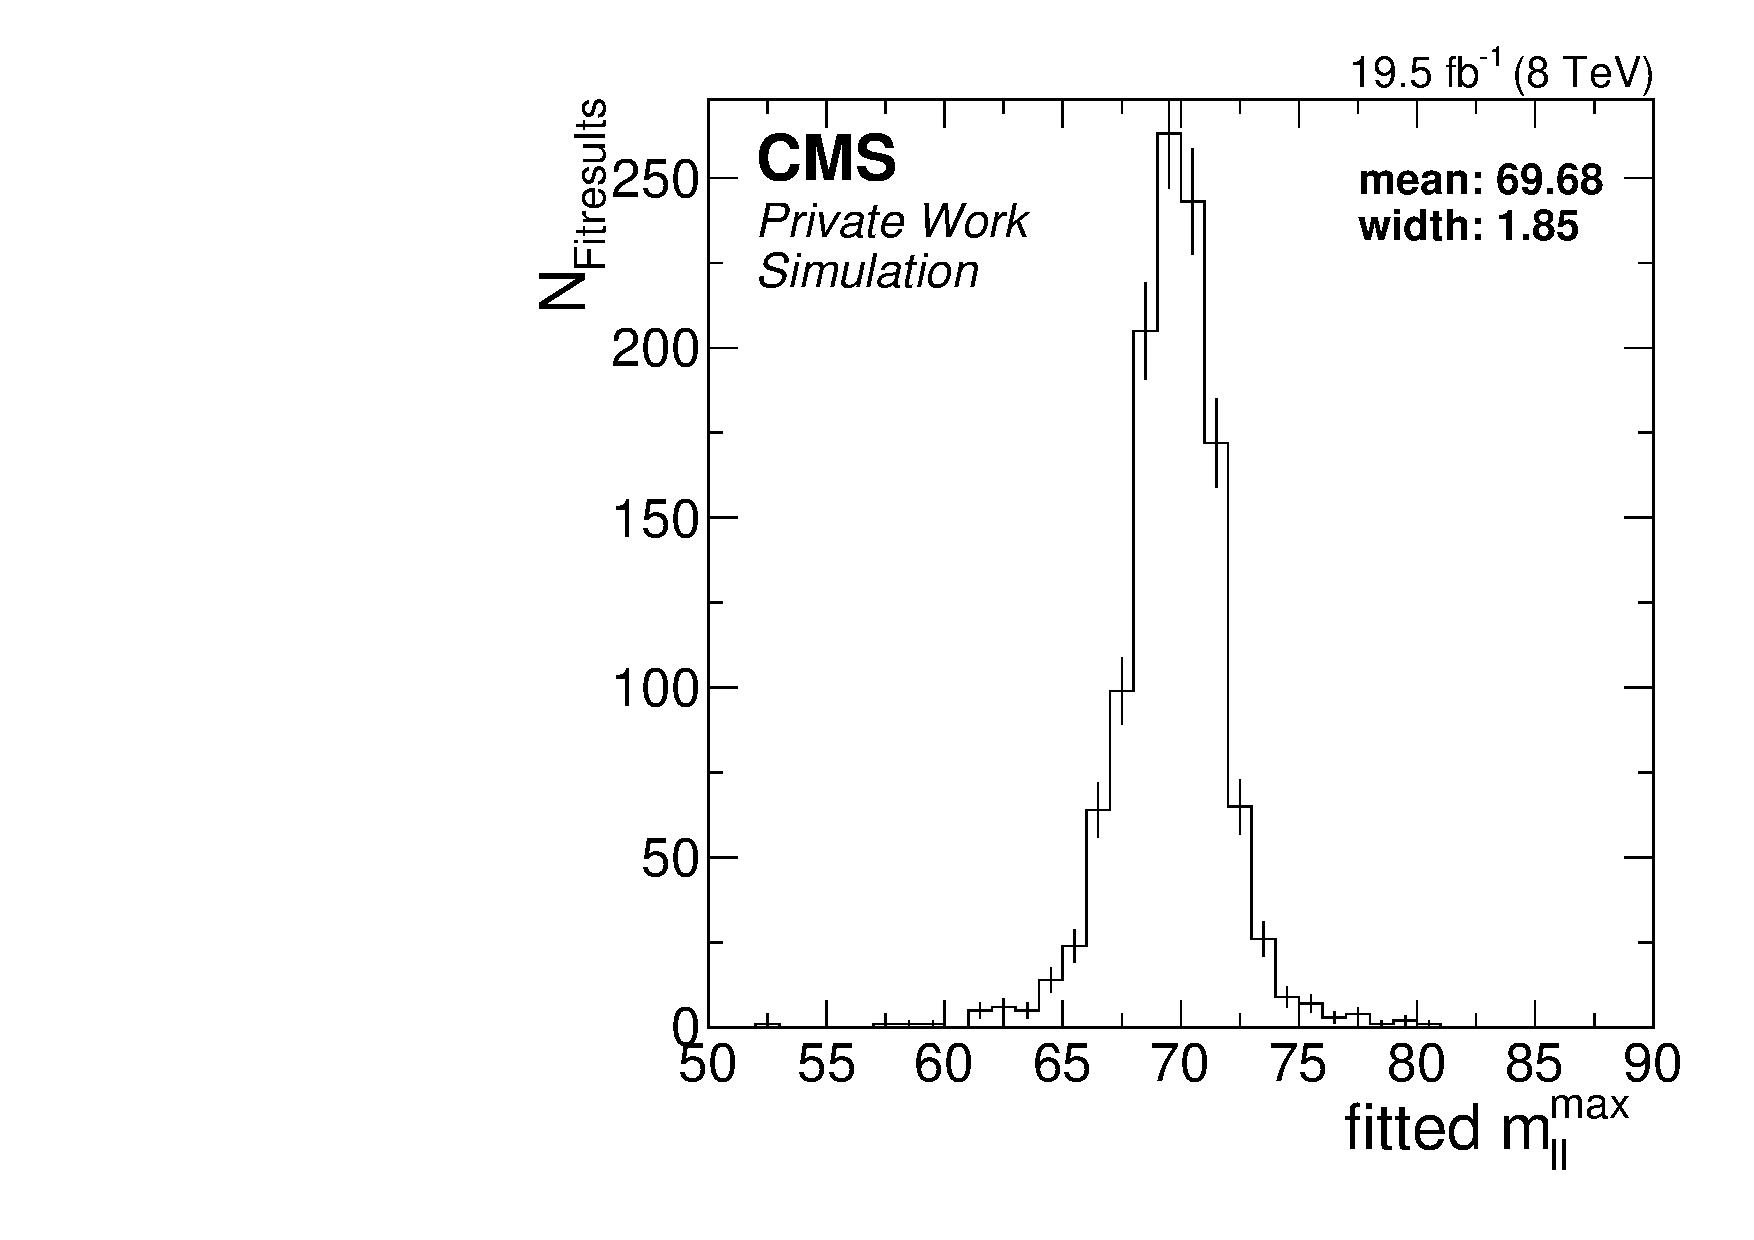
\includegraphics[width=\textwidth]{plots/results/fit/toyResults/m0_signalInjected.pdf}
  \end{minipage}
  \begin{minipage}[t]{0.49\textwidth}
    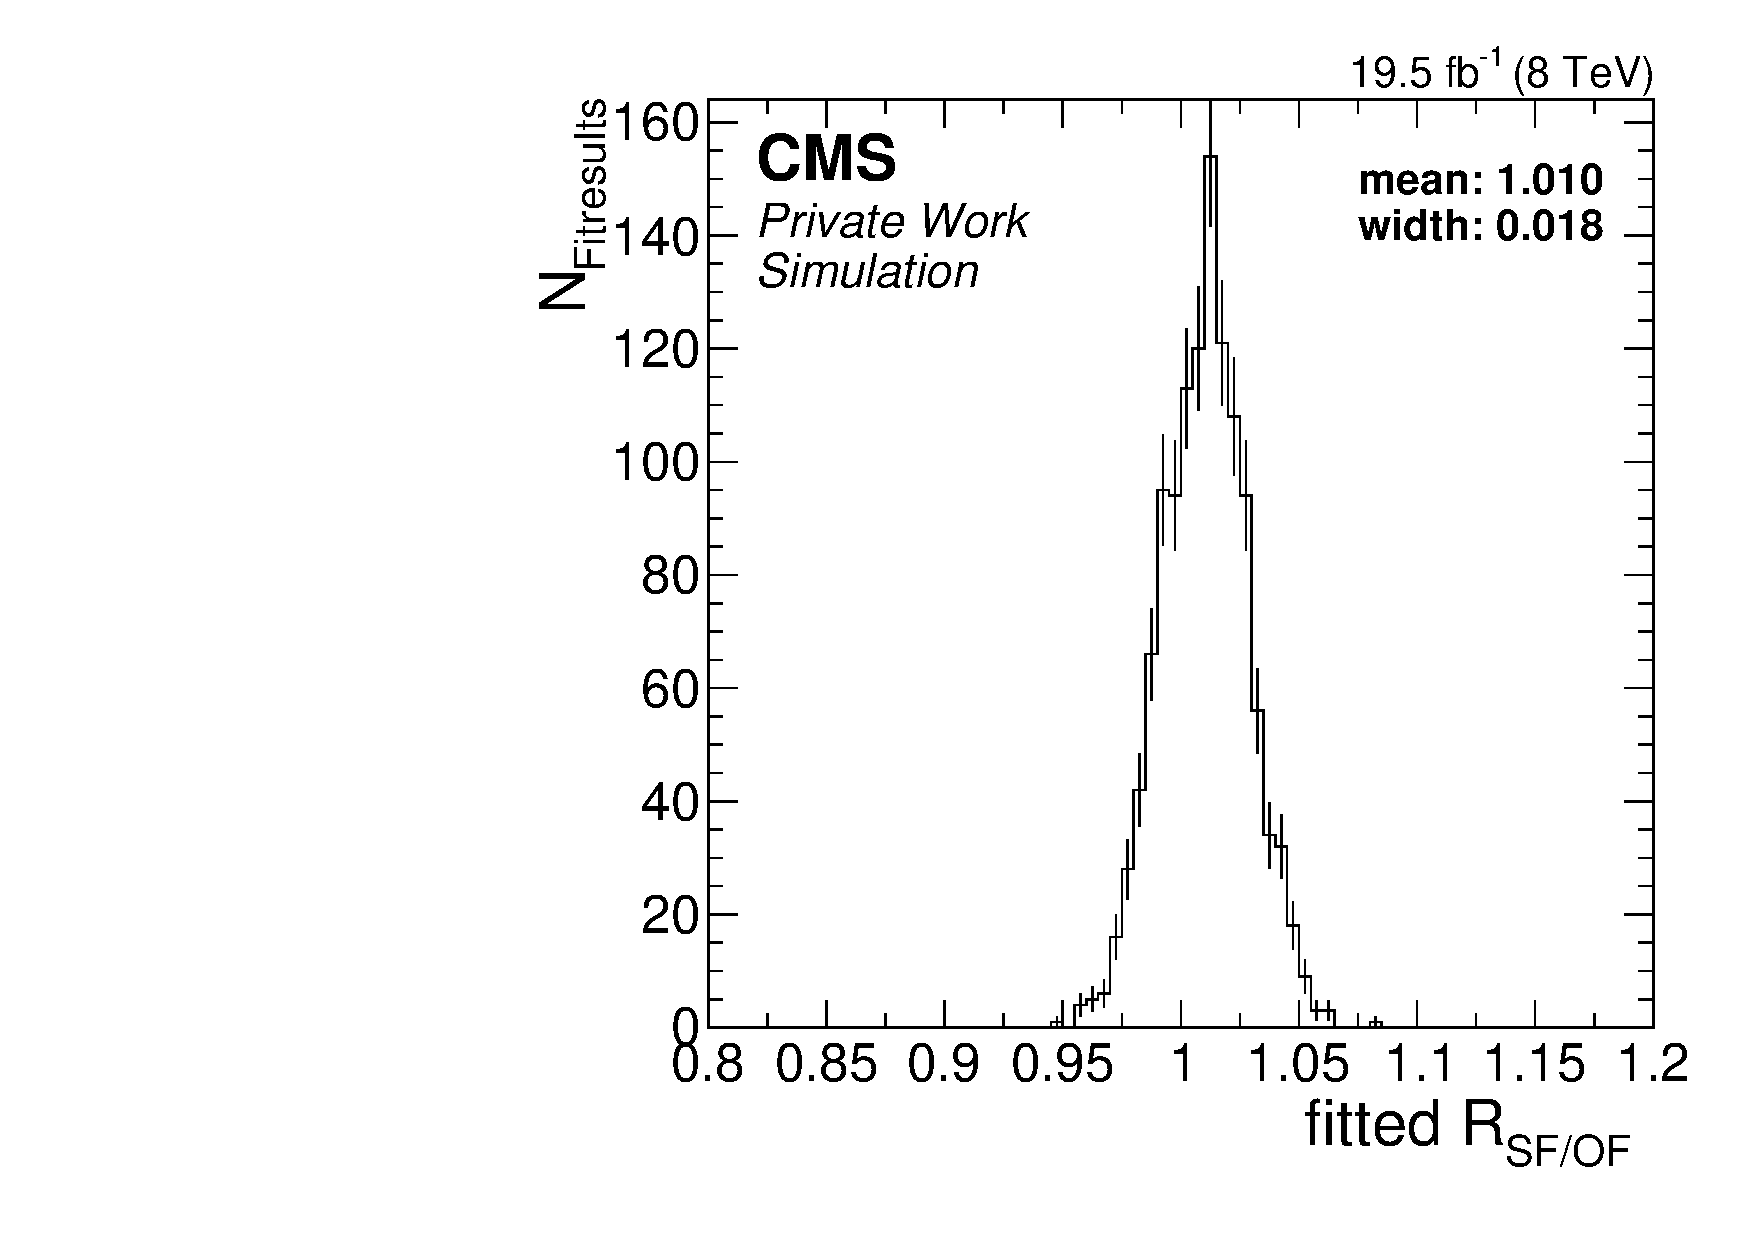
\includegraphics[width=\textwidth]{plots/results/fit/toyResults/rSFOF_signalInjected.pdf}
  \end{minipage}
  \caption{Distribution of fit observables in toy studies with a signal injected in the central signal region. Shown are the fitted number of signal events in the central region (upper left), the fitted number of signal events divided by the fitted uncertainty in the central region (upper right), the fitted edge position (lower left) and the fitted \Rsfof in the central region (lower right).}
  \label{fig:toys:signalInjected}
\end{figure}

To study the dependence of the fit result on the edge position, toys are generated with a signal of 125 events, again fluctuated according to a Poisson distribution, in the central signal region, injected at different values of \mlledge between 40 and 200\GeV in steps of 10\GeV. For each configuration, about 1000 fits are performed. The initial value of \mlledge is chosen to coincide with the generated one. The distributions of the fitted \mlledge and number of signal events for each generated \mlledge are shown in Figure~\ref{fig:toys:scan}. In the case of the fitted \mlledge on the left side, the generated value is in general very well reproduced by the fit. The best results are obtained for low values of \mlledge, as the signal shape is much steeper and easier to separate from the background than for higher values. Towards higher values the spread of the results and especially the probability for very large deviations from the generated value increases, before they decrease towards very high values of the generated \mlledge. A notable feature is observed for generated values of 100\GeV, where for a small number of fits, the fitted value is very close to the \Z boson mass. However, the fact that the initial value is set to the correct position a priori introduces a bias towards better performance. This is demonstrated for the example of an injected signal at $\unit{\mlledge = 70}{\giga\electronvolt}$ in Figure~\ref{fig:toys:randM0Signal}, where the fitted value is plotted versus the initial value of \mlledge. For initial values below $m_{\Z}$, the correct edge position is found with a high probability. If the initial value is located on the other side of the \Z boson peak, it is much less likely to find the signal at its injected position. 

Similar behaviour is also observed for the number of fitted signal events, as shown on the right side of Figure~\ref{fig:toys:scan}. Here, the relative size of the deviation from the generated value is much larger as in the case of \mlledge, as the event yields are fluctuated in the generation of the toys. 
\begin{figure}[htbp]
  \centering
  \begin{minipage}[t]{0.49\textwidth}
    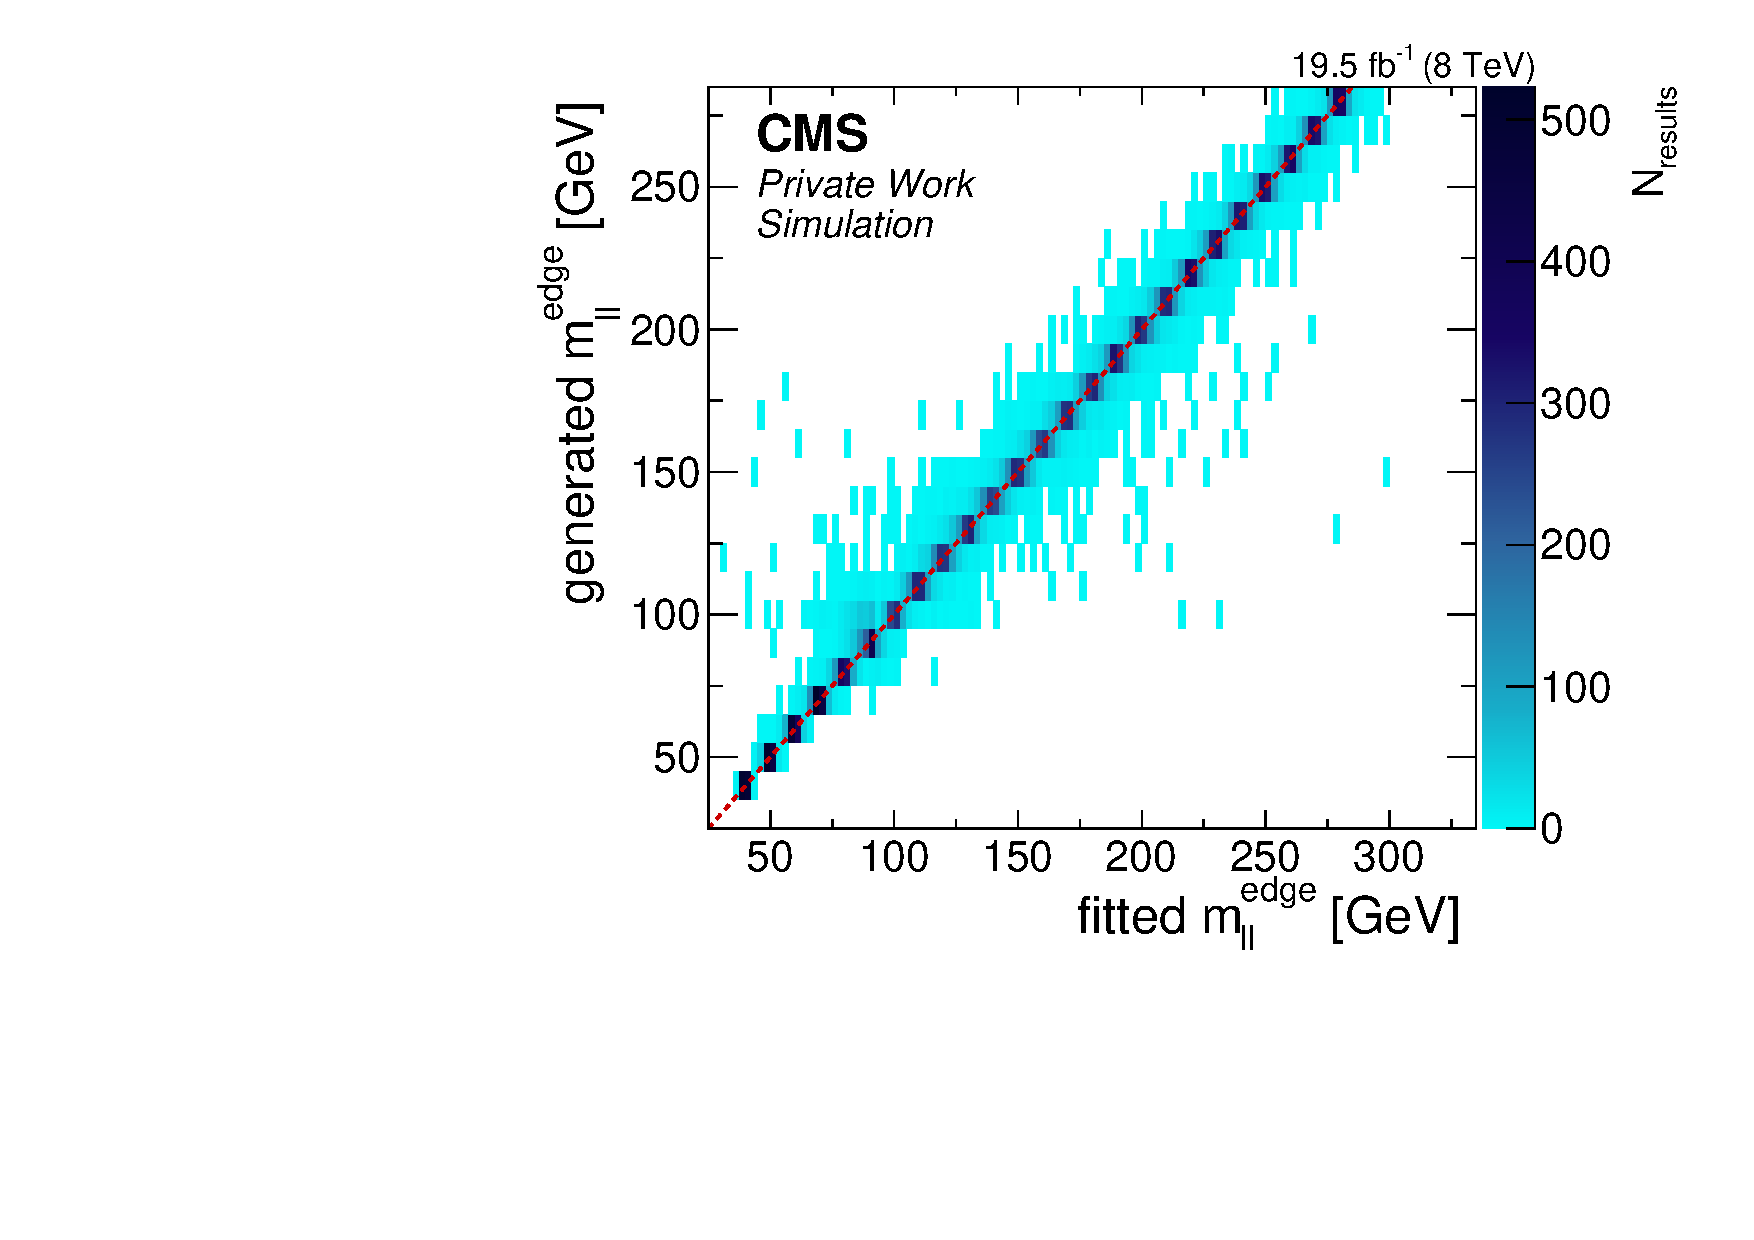
\includegraphics[width=\textwidth]{plots/results/fit/toyResults/generatedM0vsfittedM0_signalInjectedN125.pdf}
  \end{minipage}
  \begin{minipage}[t]{0.49\textwidth}
    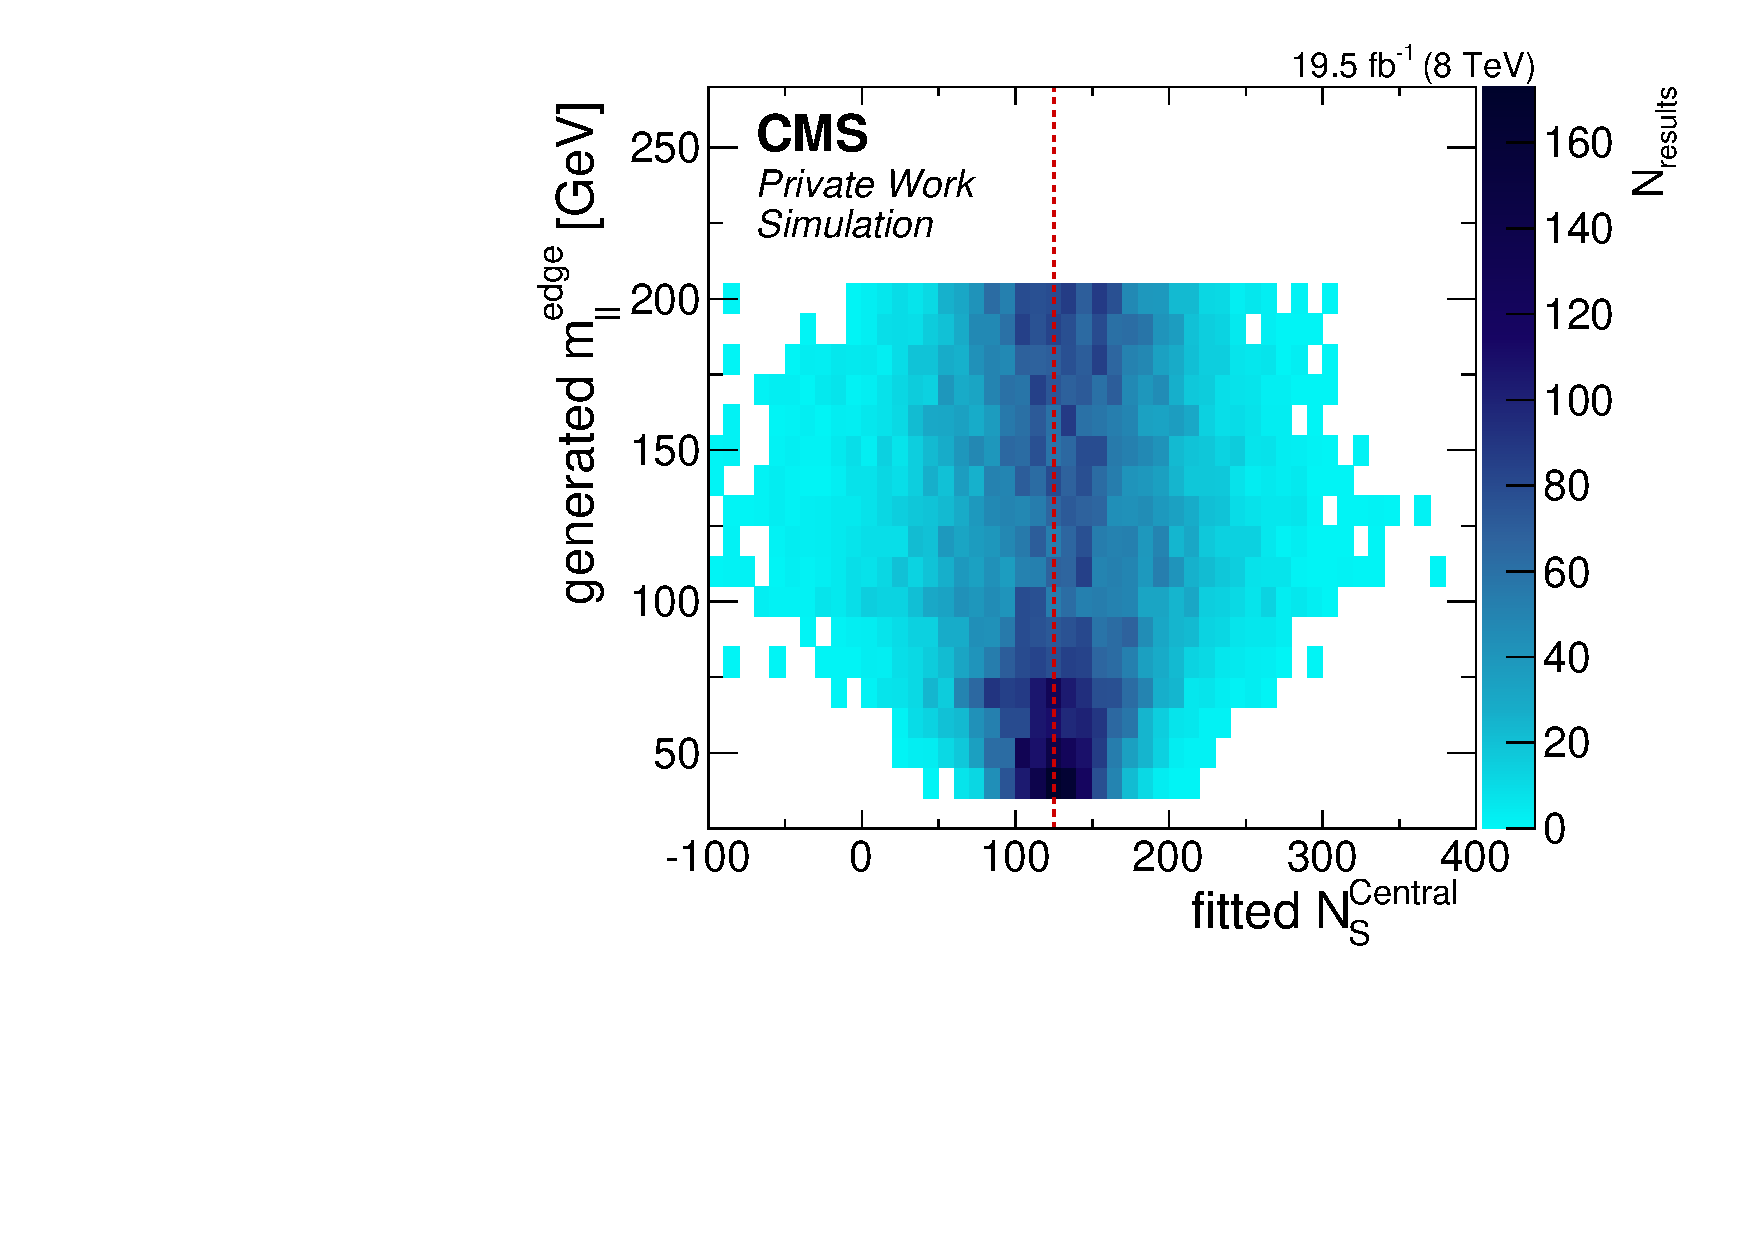
\includegraphics[width=\textwidth]{plots/results/fit/toyResults/generatedM0vsfittedNS_signalInjectedN125.pdf}
  \end{minipage}
  \caption{Distributions of the fitted \mlledge (left) and the number of signal events (right) for each generated \mlledge. The frequency of the results is colour-coded, darker colours indicating higher values. The dashed red lines indicate the points at which the fitted result matches the generated value.}
    \label{fig:toys:scan}
\end{figure}

The width of the distribution of the fitted \mlledge is shown on the left side of Figure~\ref{fig:toys:scanFits} as a function of the injected value. It is quantified both with the root mean square (RMS) of the distribution and the width of a Gaussian fitted in a range of $\pm\unit{3}{\giga\electronvolt}$ around the generated value. The first is sensitive to the non-Gaussian tails of the distribution, while the latter is a measure of the core resolution. For generated values of \mlledge of $\unit{40}{\giga\electronvolt}$, the two values are the same, but quickly deviate for higher edge positions. The Gaussian width rises from about $\unit{1}{\giga\electronvolt}$ to about $\unit{2-2.5}{\giga\electronvolt}$ for edge position above $\unit{80}{\giga\electronvolt}$ and is roughly constant for higher edge positions. The RMS reaches values of $\unit{4}{\giga\electronvolt}$ for edges below the Z mass. For $\unit{\mlledge=100}{\giga\electronvolt}$ the width is much larger, caused by the bias towards the \Z boson mass observed in Figure~\ref{fig:toys:scan}. Above the \Z boson peak, the RMS of the distribution is roughly stable at $\unit{8}{\giga\electronvolt}$, before it drops off again for edge positions above $\unit{180}{\giga\electronvolt}$. Here, the separation between \mlledge, where most of the signal is located, and the \Z boson peak becomes large.

\begin{figure}[hbp]
  \centering

    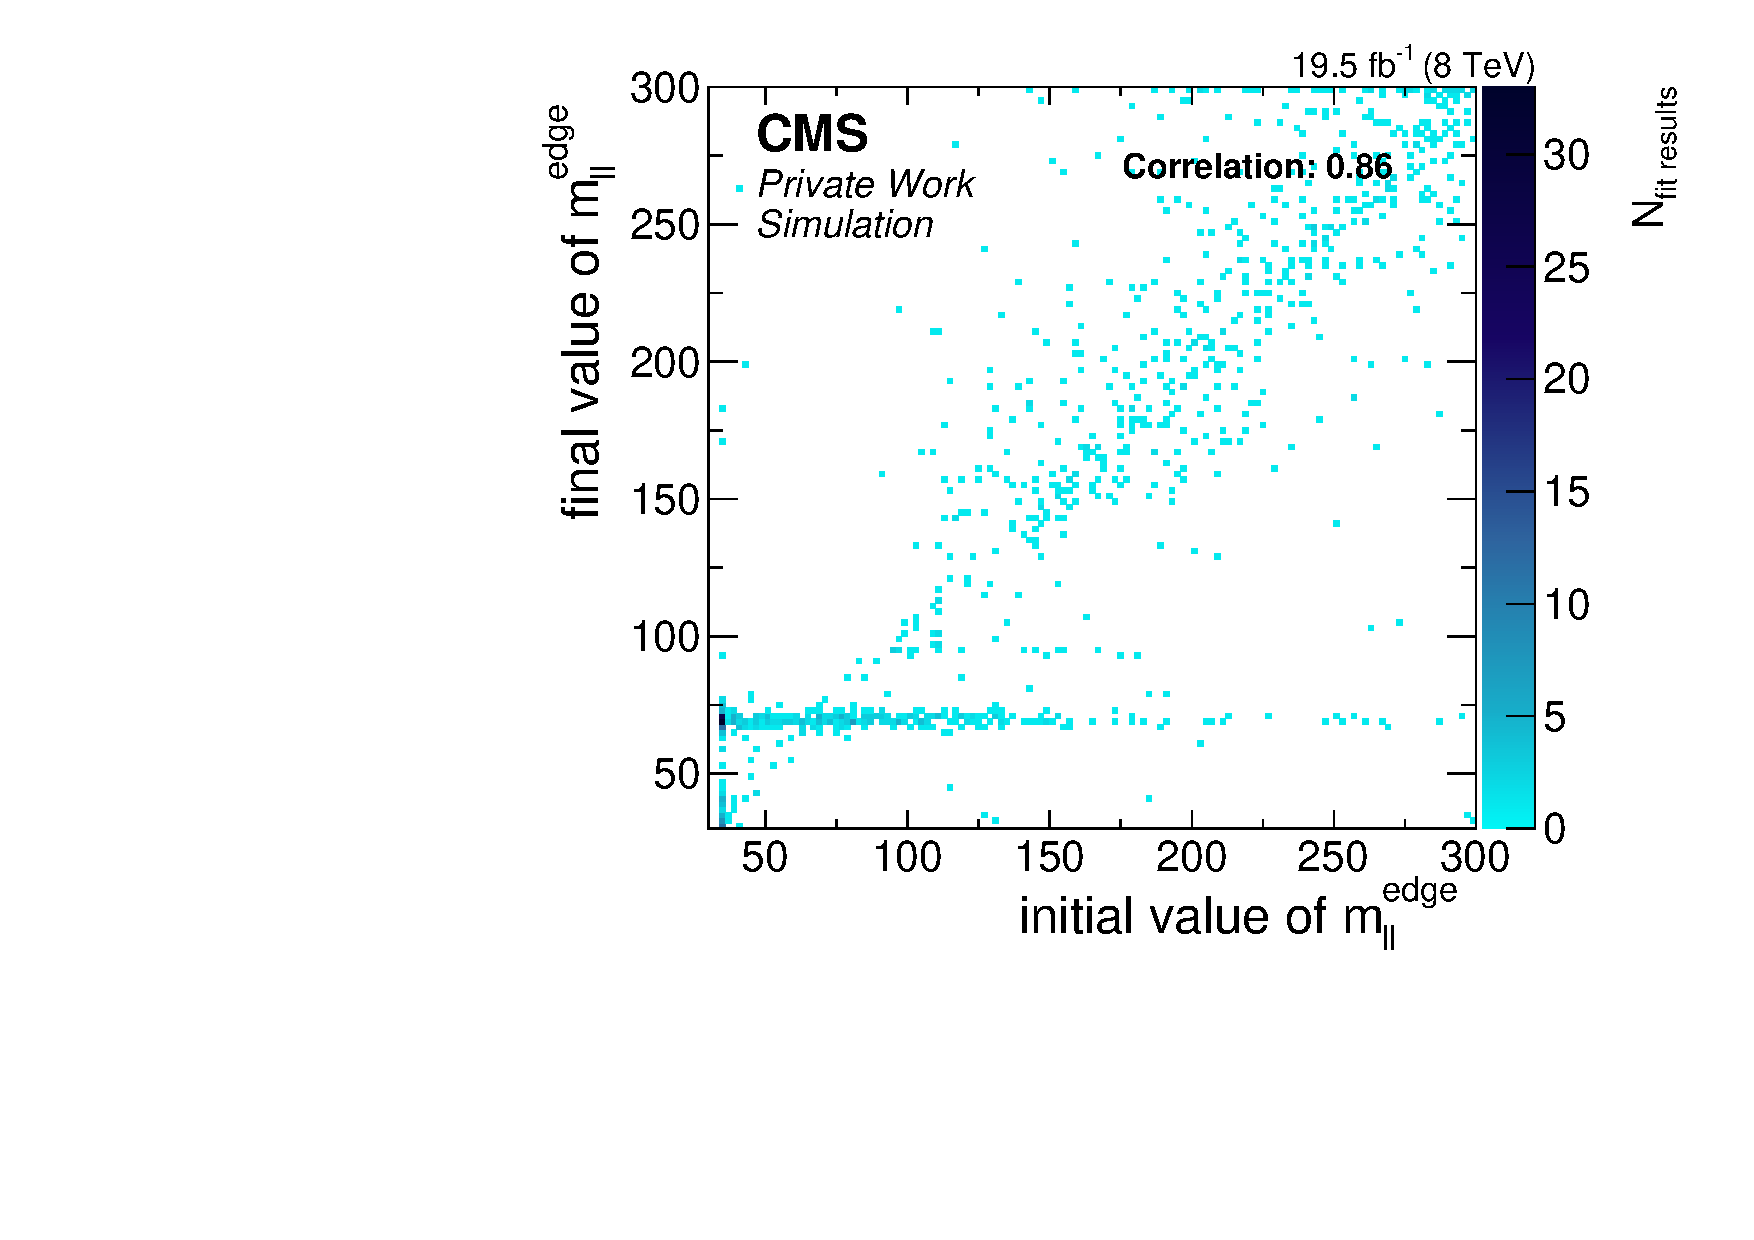
\includegraphics[width=0.6\textwidth]{plots/results/fit/toyResults/fittedM0vsinitialM0_signalInjectedM70N125_NegSig.pdf}
  \caption{Distribution of fitted versus initial values of \mlledge in the case of the randomised initial values for toys with an injected signal at $\unit{\mlledge = 70}{\giga\electronvolt}$.}
  \label{fig:toys:randM0Signal}
\end{figure}

The right side of Figure~\ref{fig:toys:scanFits} shows the means and widths of fits of Gaussian functions to the distributions of $N_{S}^{central}$, again as a function of the generated \mlledge. The distributions do not exhibit significant non-Gaussian tails, so the RMS value is not shown in this case. The injected value, fluctuated around 125 events, is reproduced within about 8 events for all values of \mlledge. The width increases with \mlledge from roughly 25 to 65 events at \mlledge of $\unit{100}{\giga\electronvolt}$ and decreases slightly for higher values.

\begin{figure}[!hbp]
  \centering
  \begin{minipage}[t]{0.49\textwidth}
    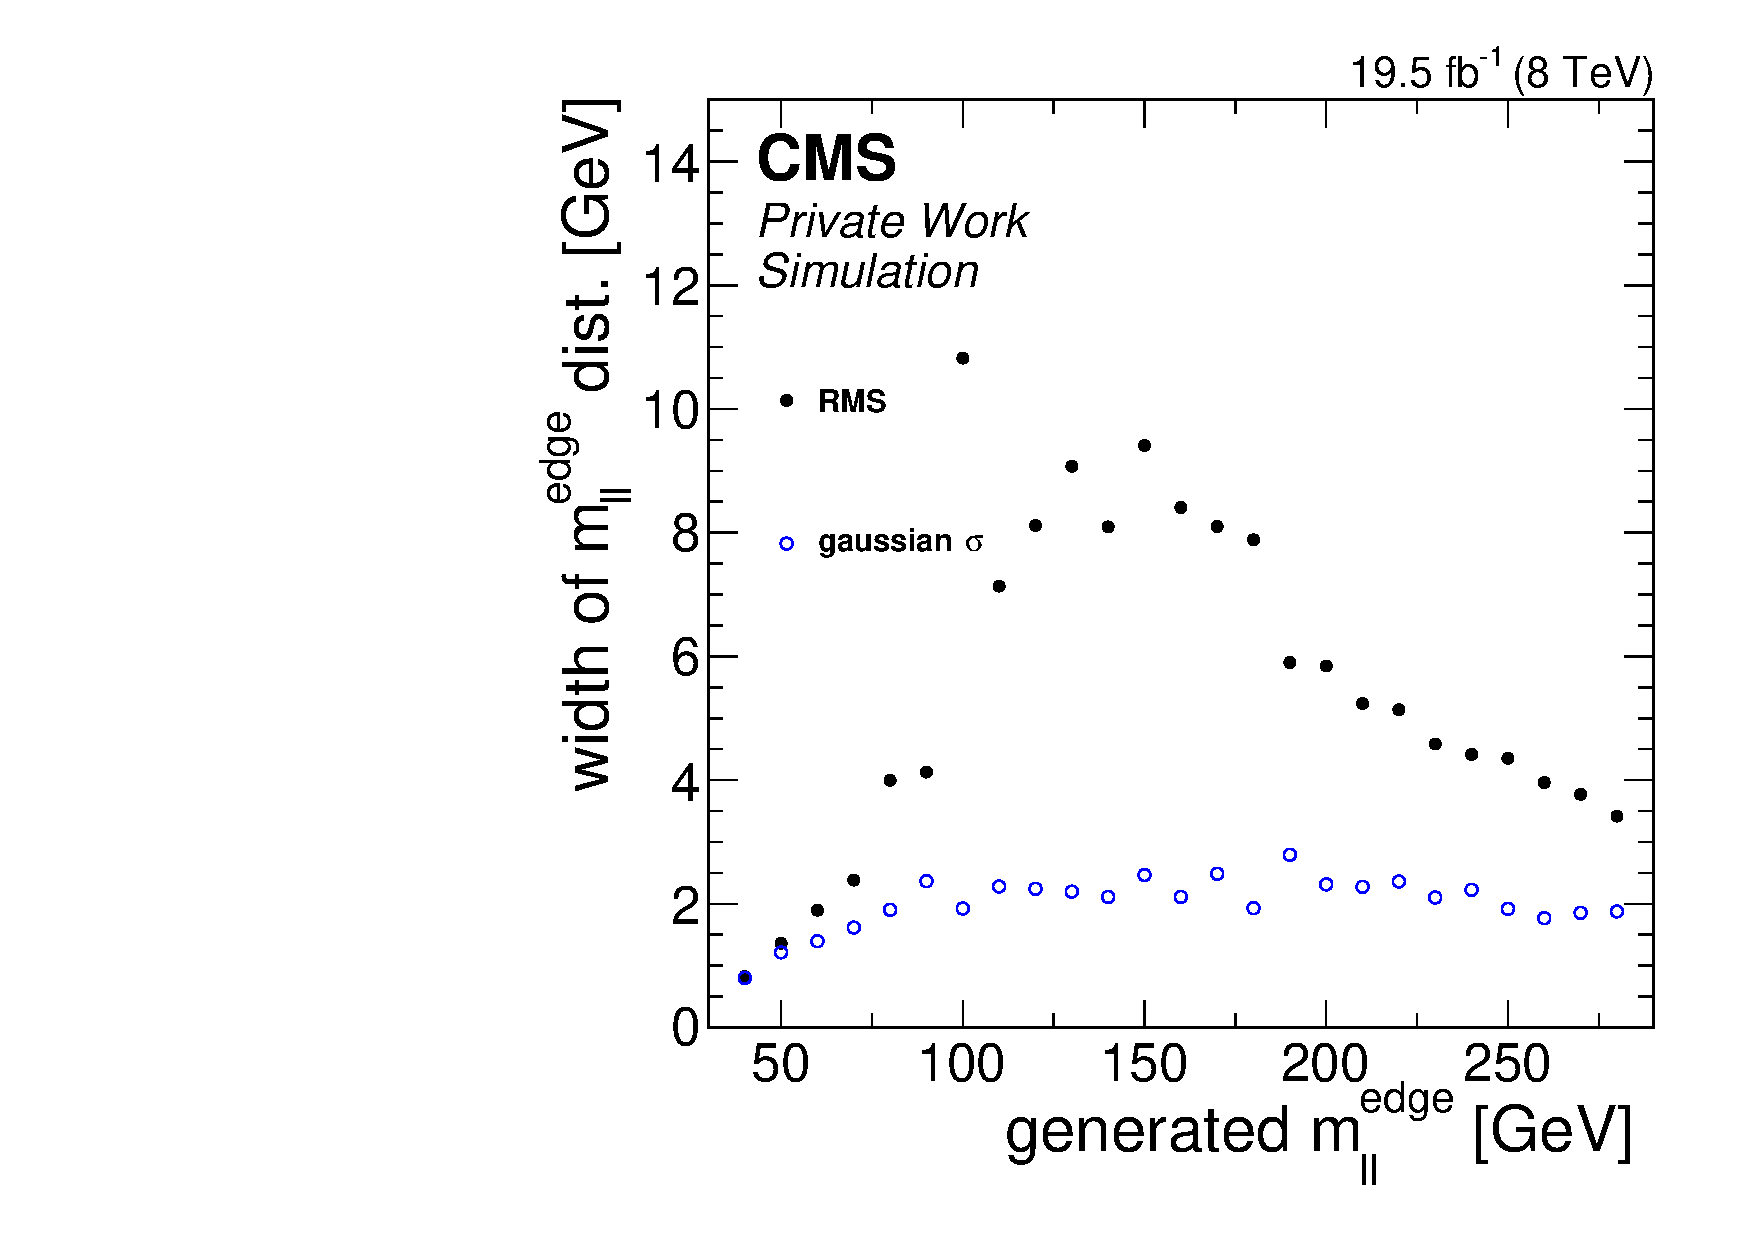
\includegraphics[width=\textwidth]{plots/results/fit/toyResults/WidthsvsGenM0Ratio_signalInjectedN125.pdf}
  \end{minipage}
  \begin{minipage}[t]{0.49\textwidth}
    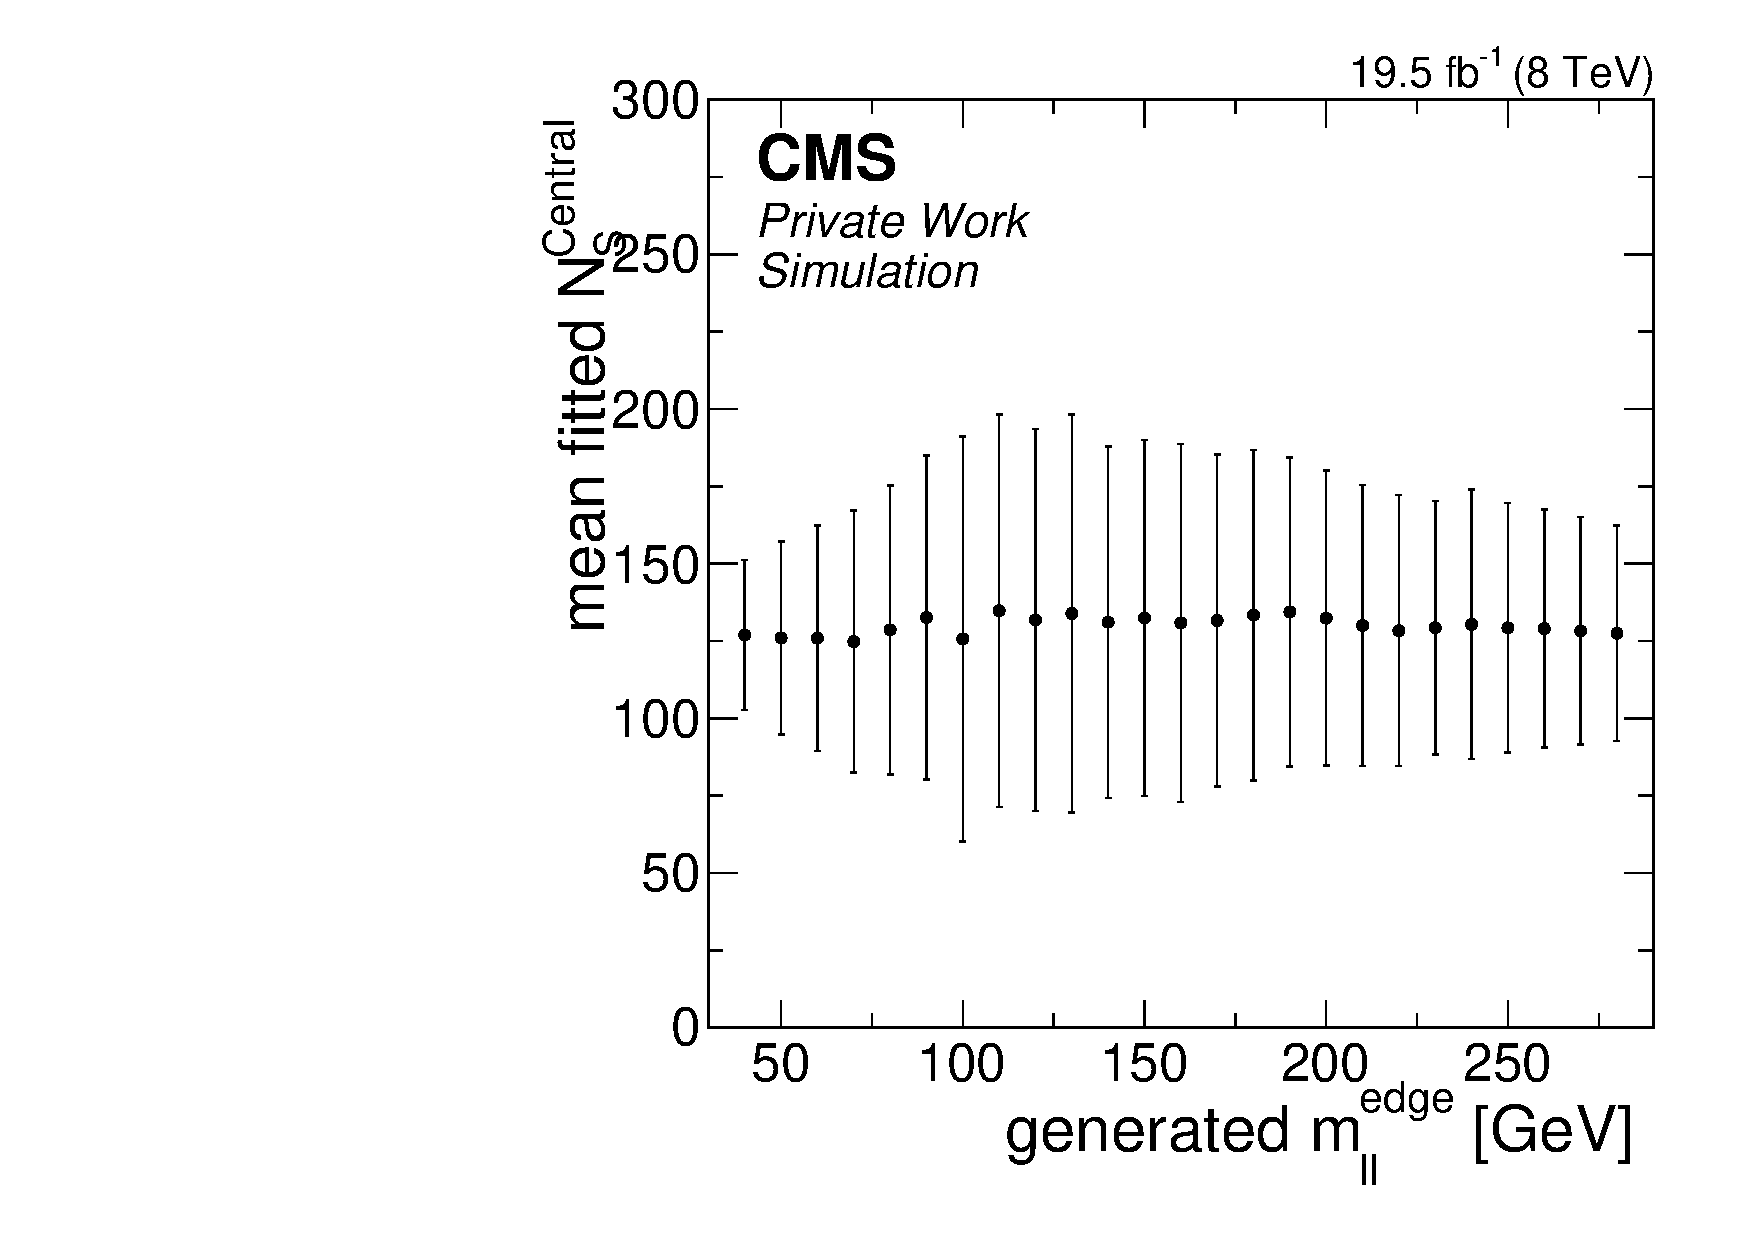
\includegraphics[width=\textwidth]{plots/results/fit/toyResults/meanNSvsGenM0_signalInjectedN125.pdf}
  \end{minipage}
  \caption{Fitted widths of the \mlledge (left) and means and widths of the $N_S^{central}$ distributions (right) as a function of the generated \mlledge.}
    \label{fig:toys:scanFits}
\end{figure}

To test deviations from the assumed signal shape, toys are generated with a signal injected at $\unit{\mlledge = 70}{\giga\electronvolt}$ and a size of 125 events, but following the convex and concave signal shapes described in Section~\ref{sec:sigModel}. The exponent $\gamma$ in Equations~\ref{eq:convex} and~\ref{eq:concave} is chosen to be 4, resulting in strong deviations from the nominal signal shape, as illustrated in Figure~\ref{fig:mc:shapes}. The toys generated in this manner are then fitted using the nominal triangular signal shape. Resulting distributions are shown in Figure~\ref{fig:toys:signalInjectedShapeBias}. When fitting a convex signal with the triangular shape a bias towards higher signal yields of 20 events is introduced, together with a preference of slightly higher values for \mlledge. This higher signal yield is achieved by systematically reducing the value of \Rsfof. Less strong effects are observed in the case of a concave signal. Here, a bias towards a reduced signal yield of about 10 events is present, together with a much wider distribution of the fitted \mlledge. In this case, no change in the distribution of the fitted \Rsfof compared to the nominal signal shape is observed. 

\begin{figure}[b]
  \centering
  \begin{minipage}[t]{0.49\textwidth}
    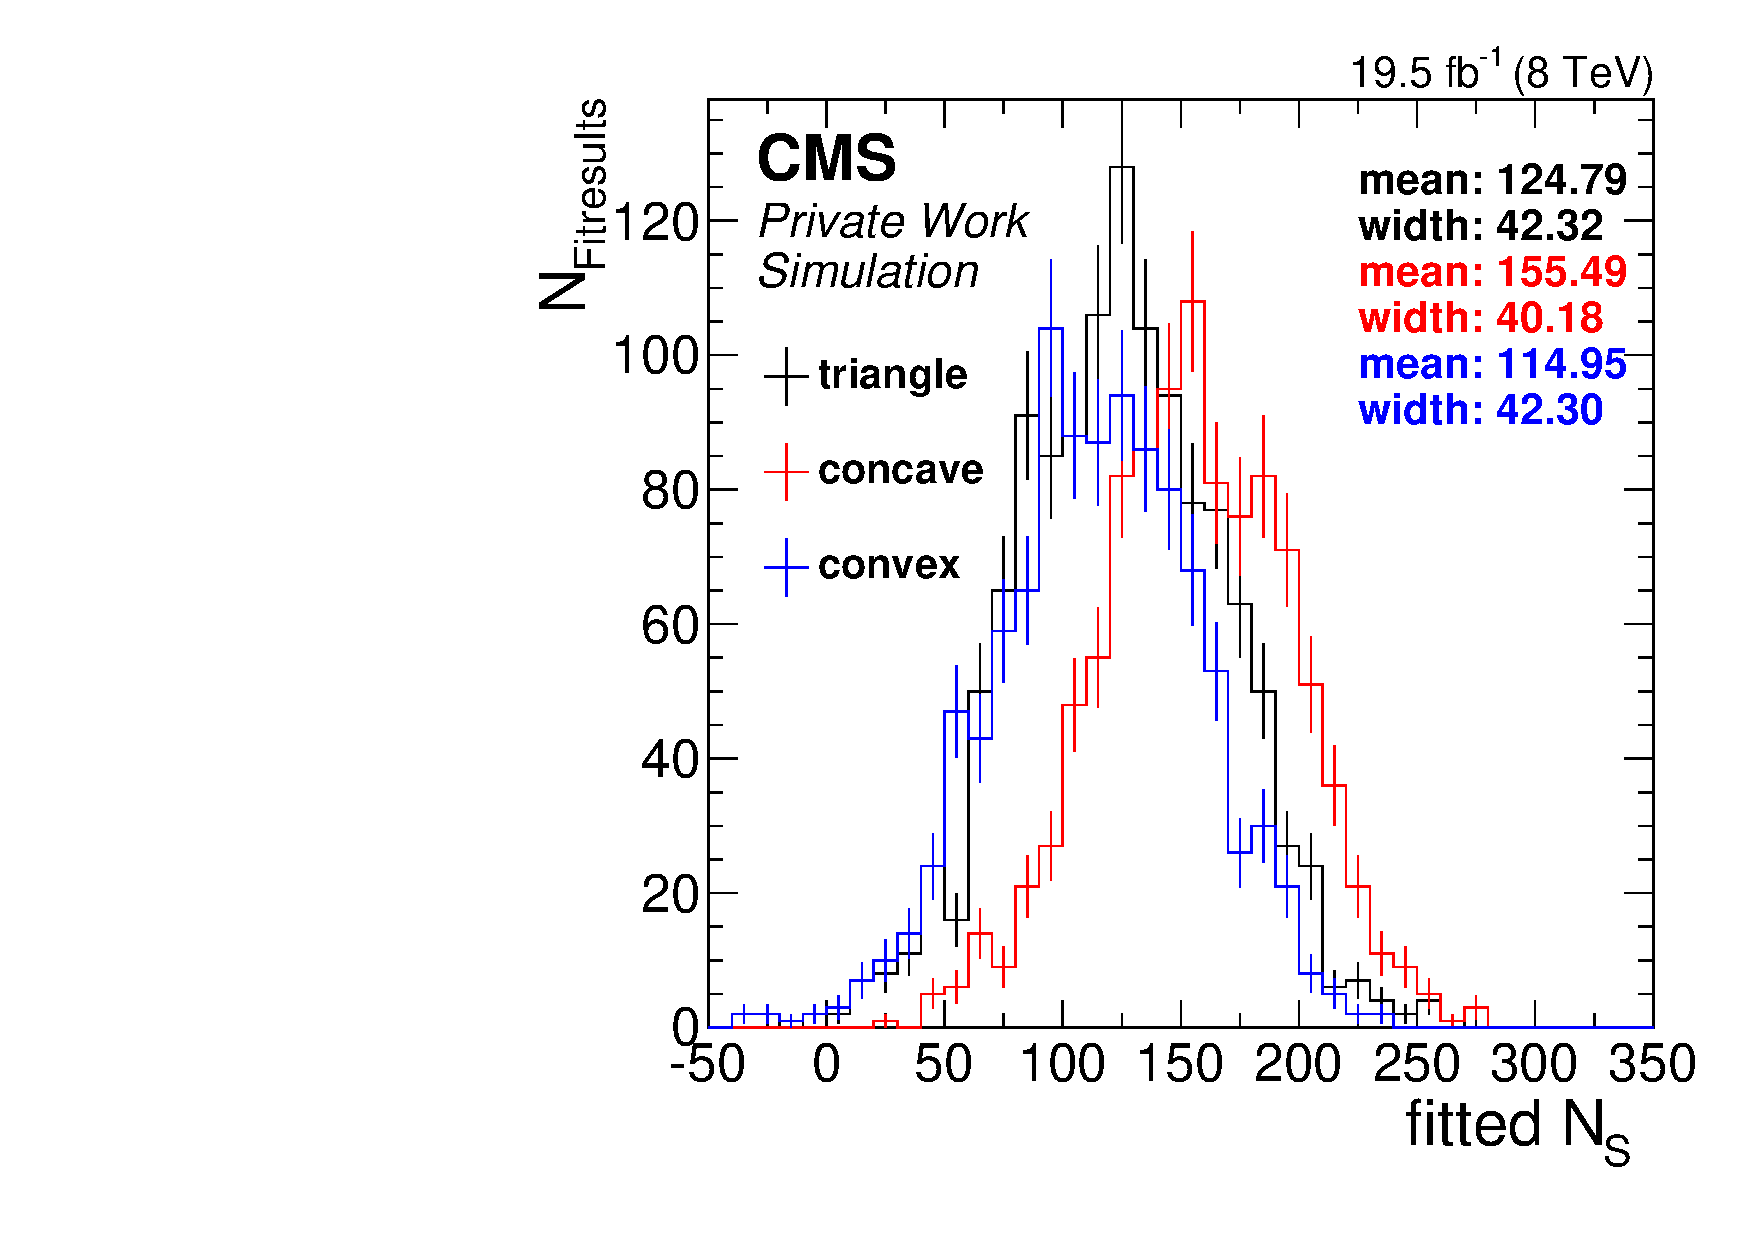
\includegraphics[width=\textwidth]{plots/results/fit/toyResults/nSPure_shapeBias.pdf}
  \end{minipage}
  \begin{minipage}[t]{0.49\textwidth}
    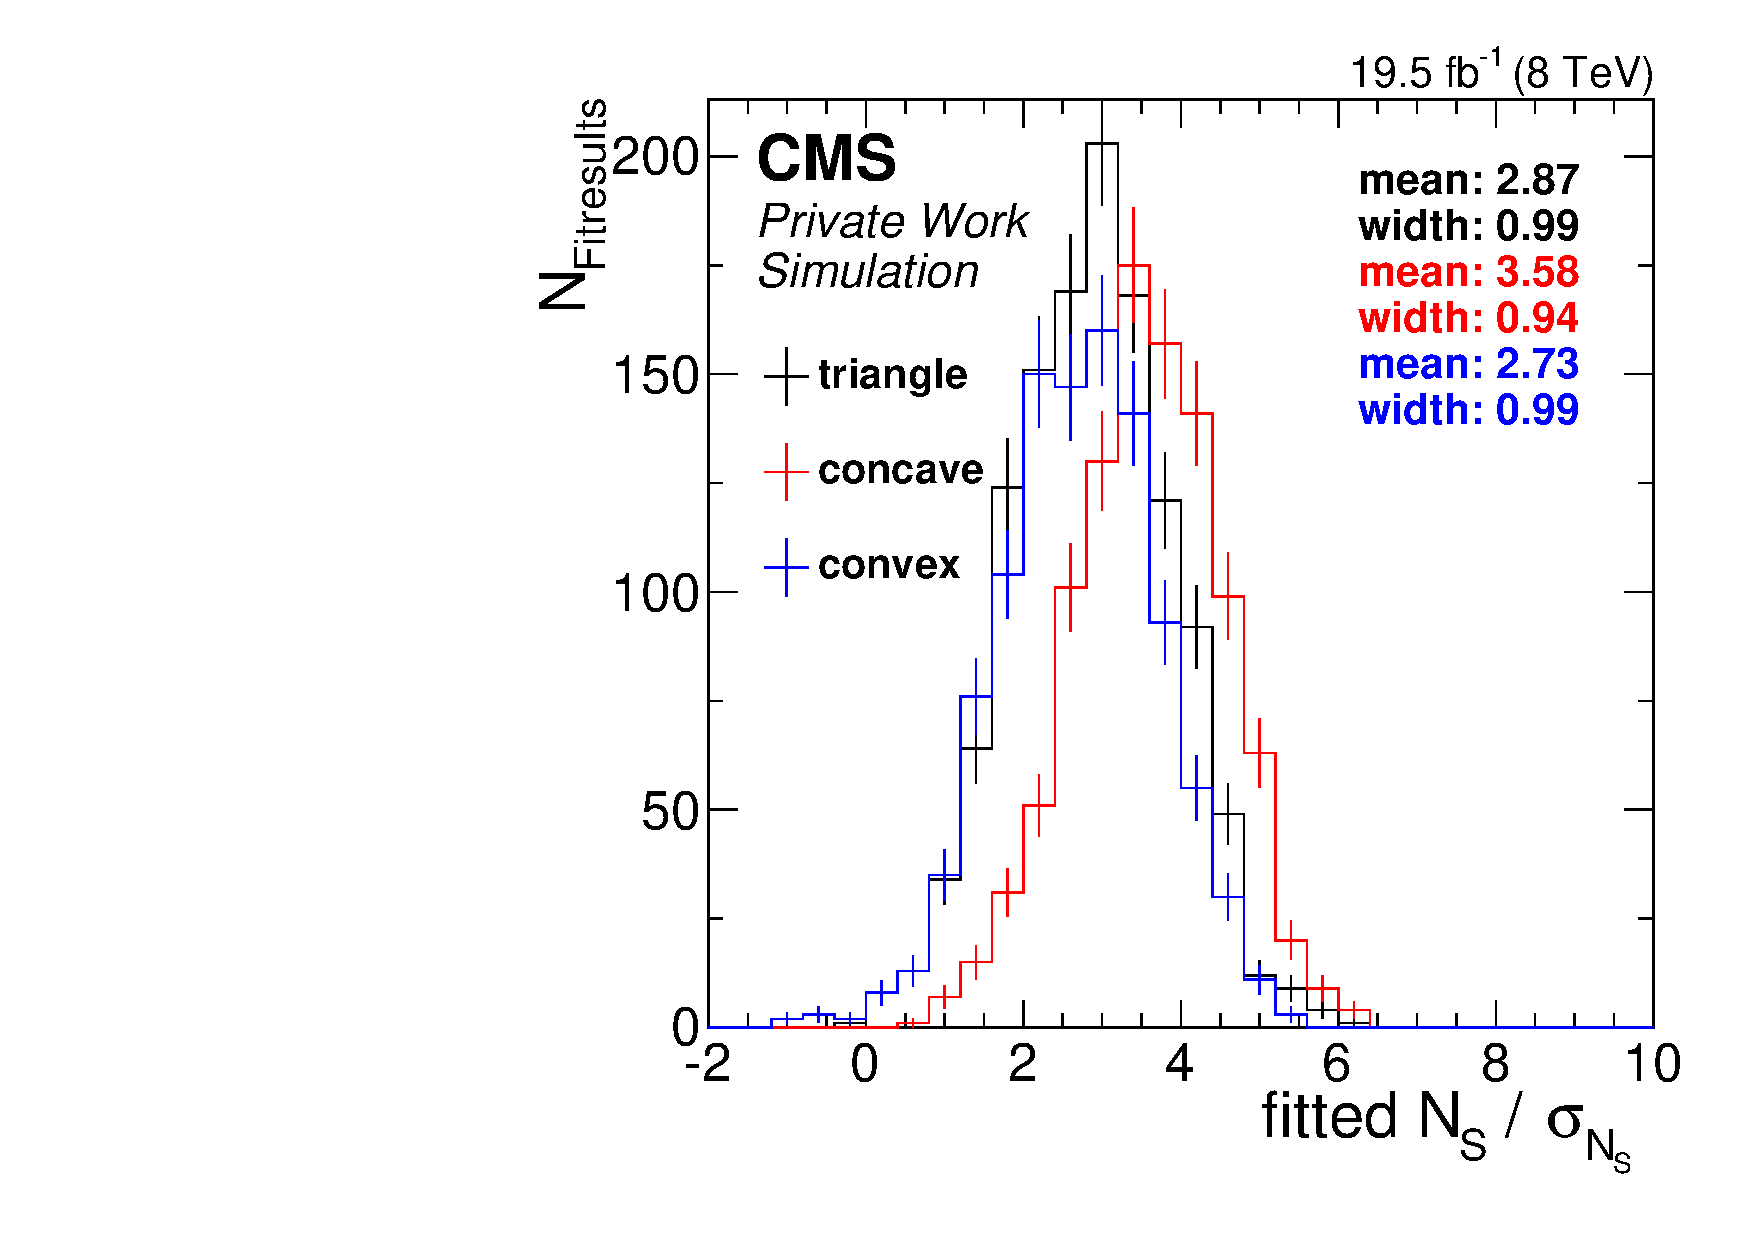
\includegraphics[width=\textwidth]{plots/results/fit/toyResults/nS_shapeBias.pdf}
  \end{minipage}
  \begin{minipage}[t]{0.49\textwidth}
    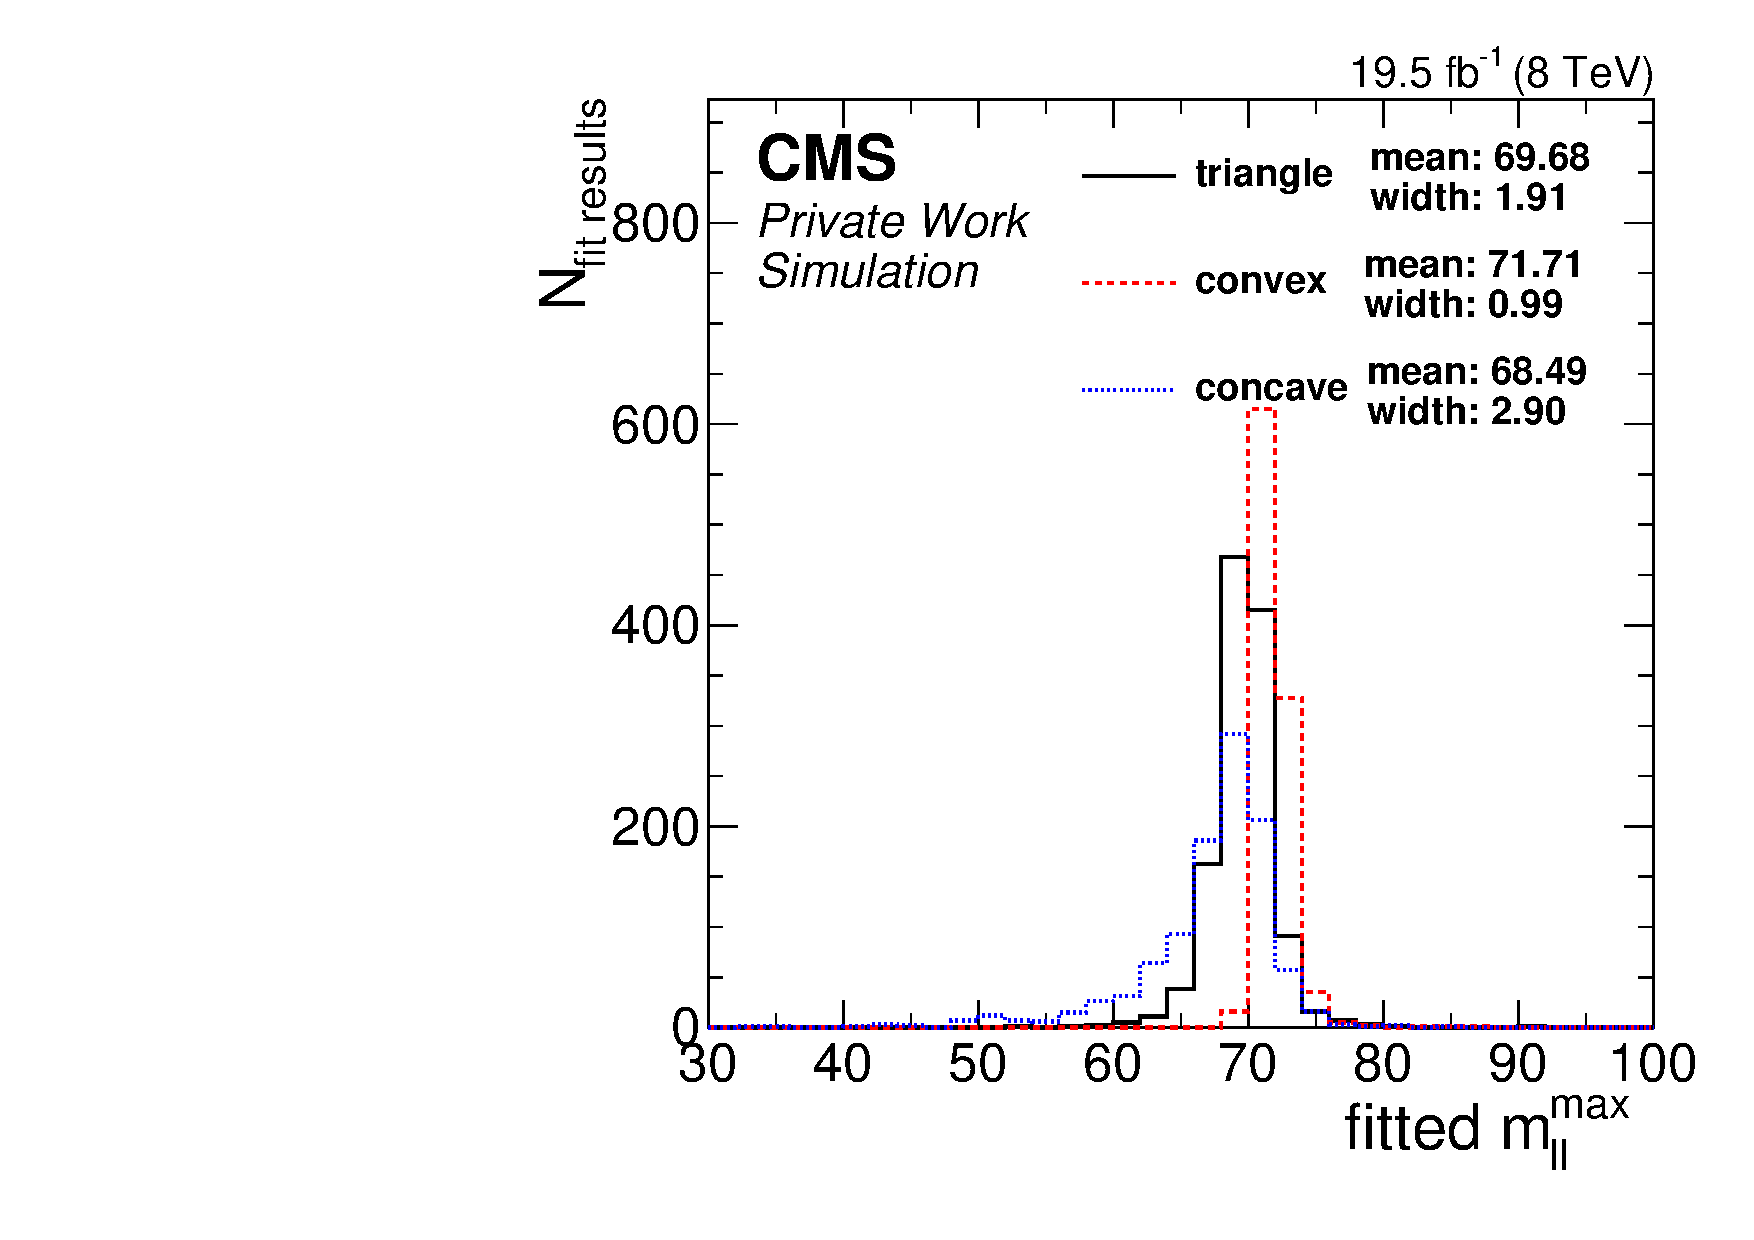
\includegraphics[width=\textwidth]{plots/results/fit/toyResults/m0_shapeBias.pdf}
  \end{minipage}
  \begin{minipage}[t]{0.49\textwidth}
    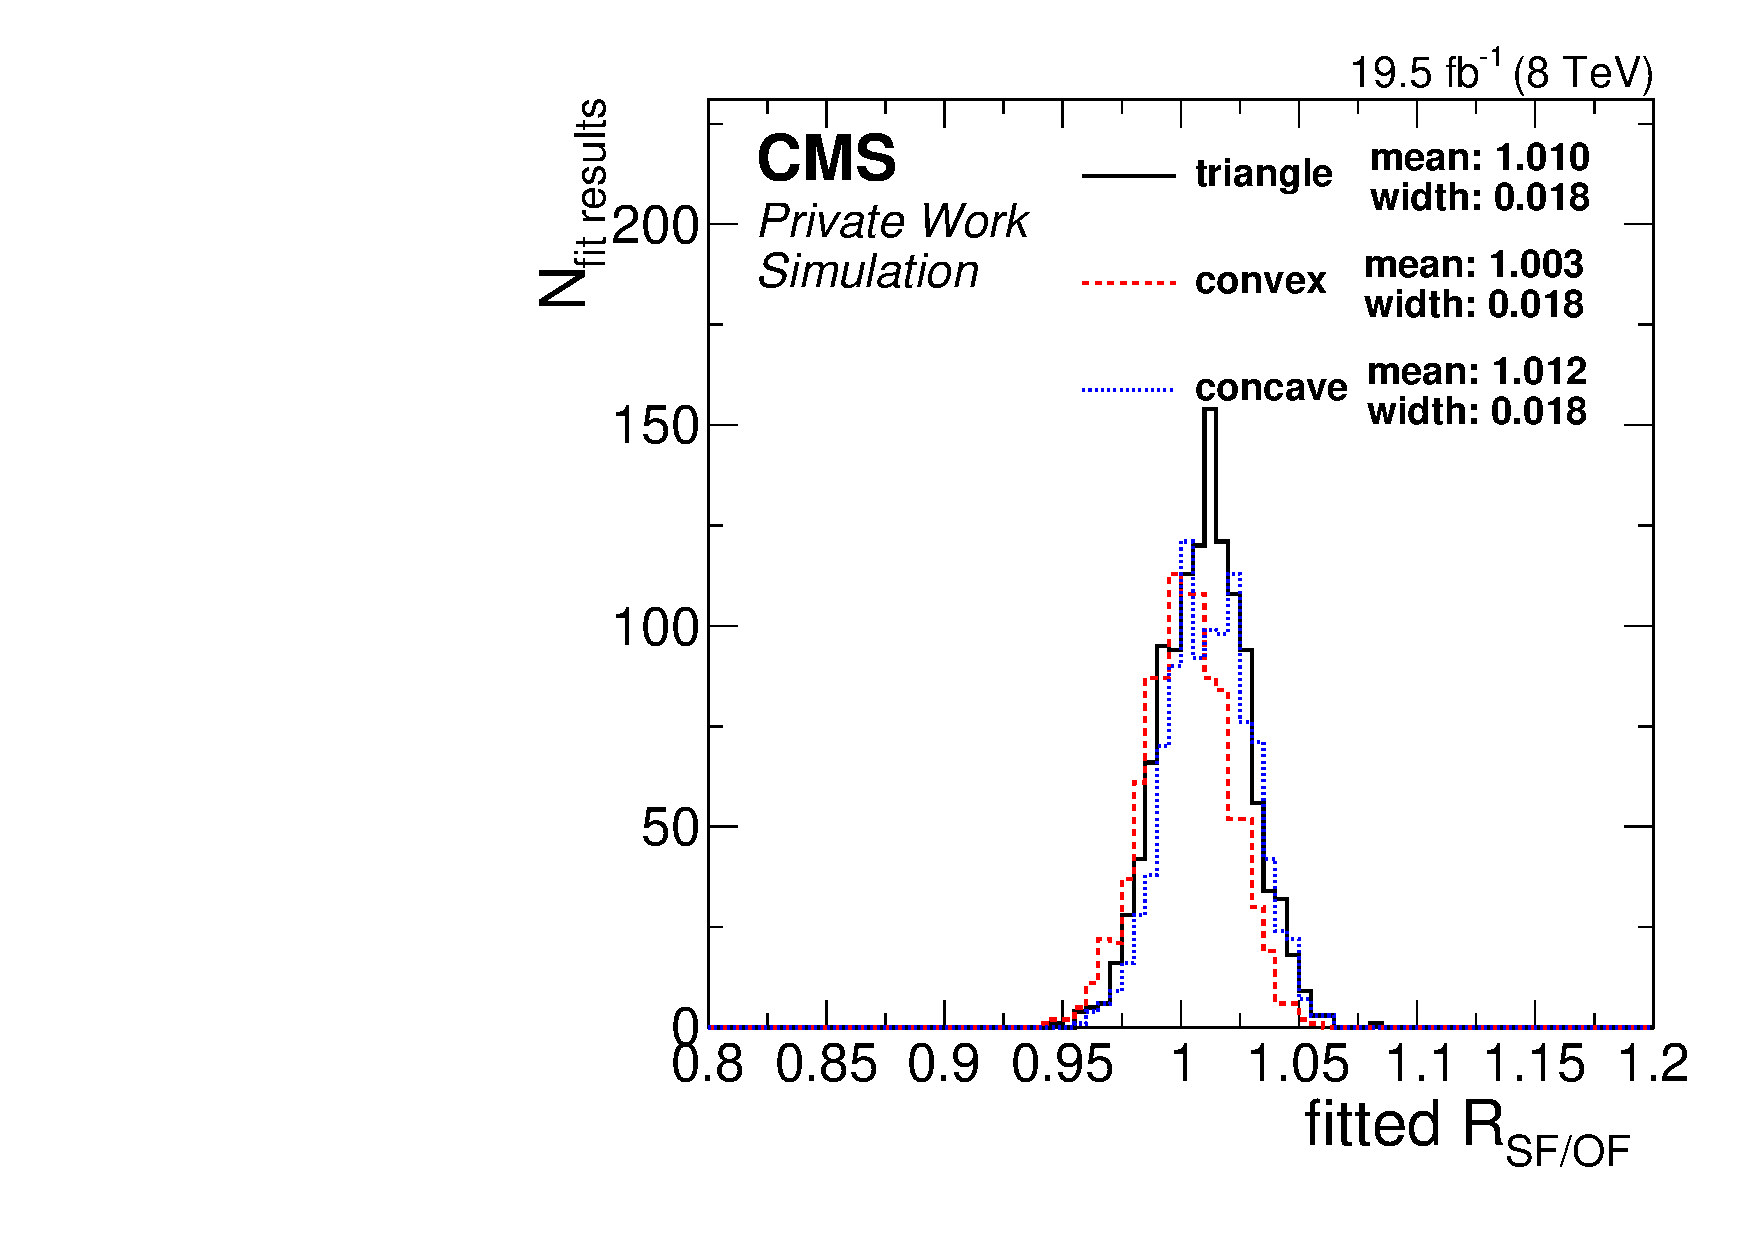
\includegraphics[width=\textwidth]{plots/results/fit/toyResults/rSFOF_shapeBias.pdf}
  \end{minipage}
  \caption{Distribution of fit observables in the central signal region in toy studies with signals following different distributions. Toys are generated using the nominal (black) as well as the concave (red) and convex (blue) signal shape. Shown are the fitted number of signal events in the central region (upper left), the fitted number of signal events divided by the fitted uncertainty in the central region (upper right), the fitted edge position (lower left), and the fitted \Rsfof in the central region (lower right).}
  \label{fig:toys:signalInjectedShapeBias}
\end{figure}

In summary, the fit shows good performance reproducing signal properties. The triangular shape has been shown to be a sufficient approximation to measure the signal yield and \mlledge. In case of a fixed edge position, the fit does not exhibit biases towards a signal. A floating edge, however, makes the fit susceptible to the look-elsewhere-effect, which has to be taken into account when assessing the significance of a result. The edge position can be measured with high precision, but it has be verified that the global minimum of the log-likelihood has been found. The variability of \Rsfof in the fit allows to at least partially correct for biases in the SF to OF mapping.
\clearpage
\section{Fit results on data}
The result of the fit performed in the signal region on data is shown in Figure~\ref{fig:fit:result}. Shown are the \mll distributions in the SF and OF channels for the central and forward dilepton selection. The quantitative results are shown in Table~\ref{tab:fitResult}. Similar to the counting experiment, an excess of events is observed below the \Z boson peak in the central signal region. The best fit value for the position of an edge is found to be $\unit{82.4}{\giga\electronvolt}$, with a signal yield of 140$\pm$44 events. No significant contribution of a signal is found in the forward region, where the fitted signal yield is 2$\pm$22 events. In the central region the fitted value of \Rsfof is slightly larger than the initial value of 1.013, indicating that the fit absorbs some fraction of the excess into the background prediction. However, the difference is small compared to the fitted uncertainty and the uncertainty on the predicted value. In the forward region, the fitted value is smaller than the initial value, but also this deviation is well within the uncertainties. 


\begin{figure}[!hbp]
  \centering
  \begin{minipage}[t]{0.49\textwidth}
    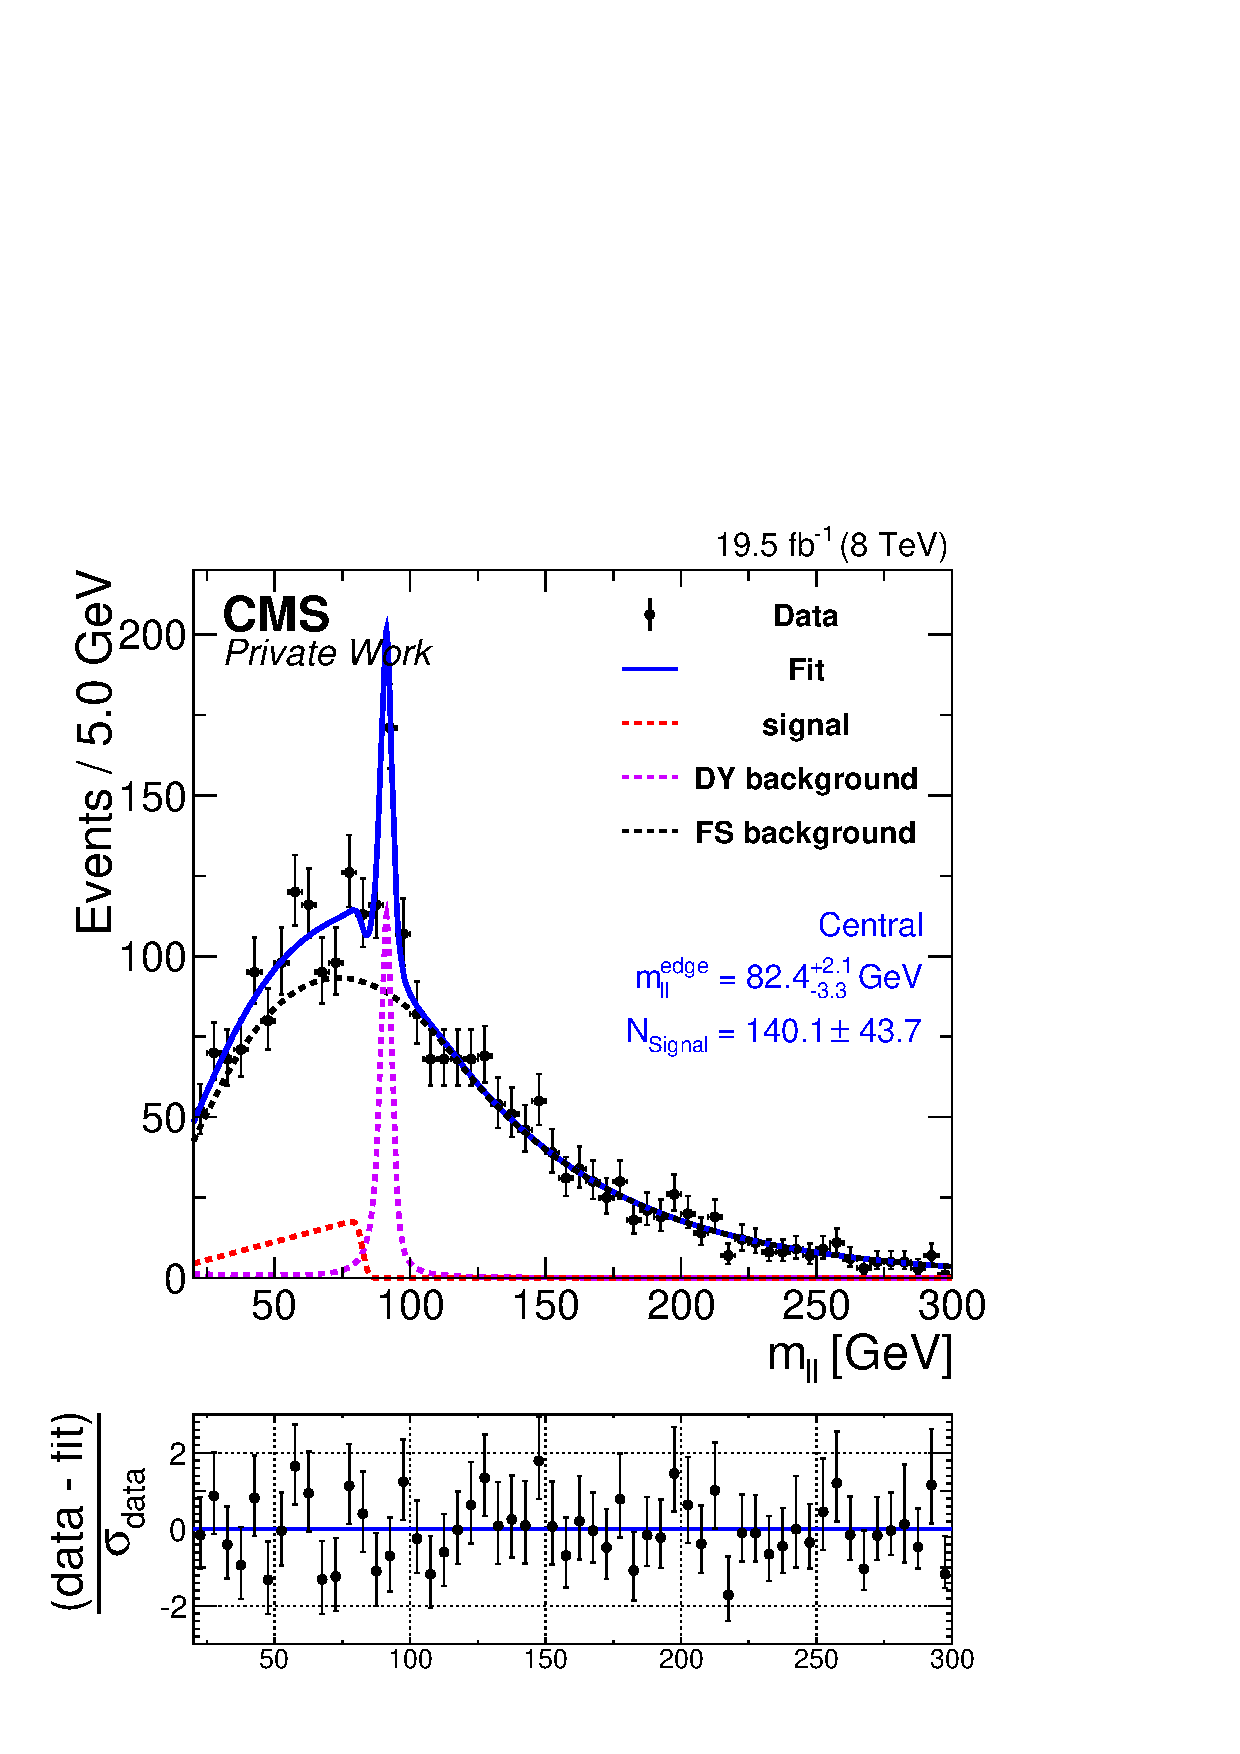
\includegraphics[width=\textwidth]{plots/results/fit/fit2012_ETHTriangle_SignalInclusive_Combined_Full2012_ETHTriangle_Central.pdf}
  \end{minipage}
  \begin{minipage}[t]{0.49\textwidth}
    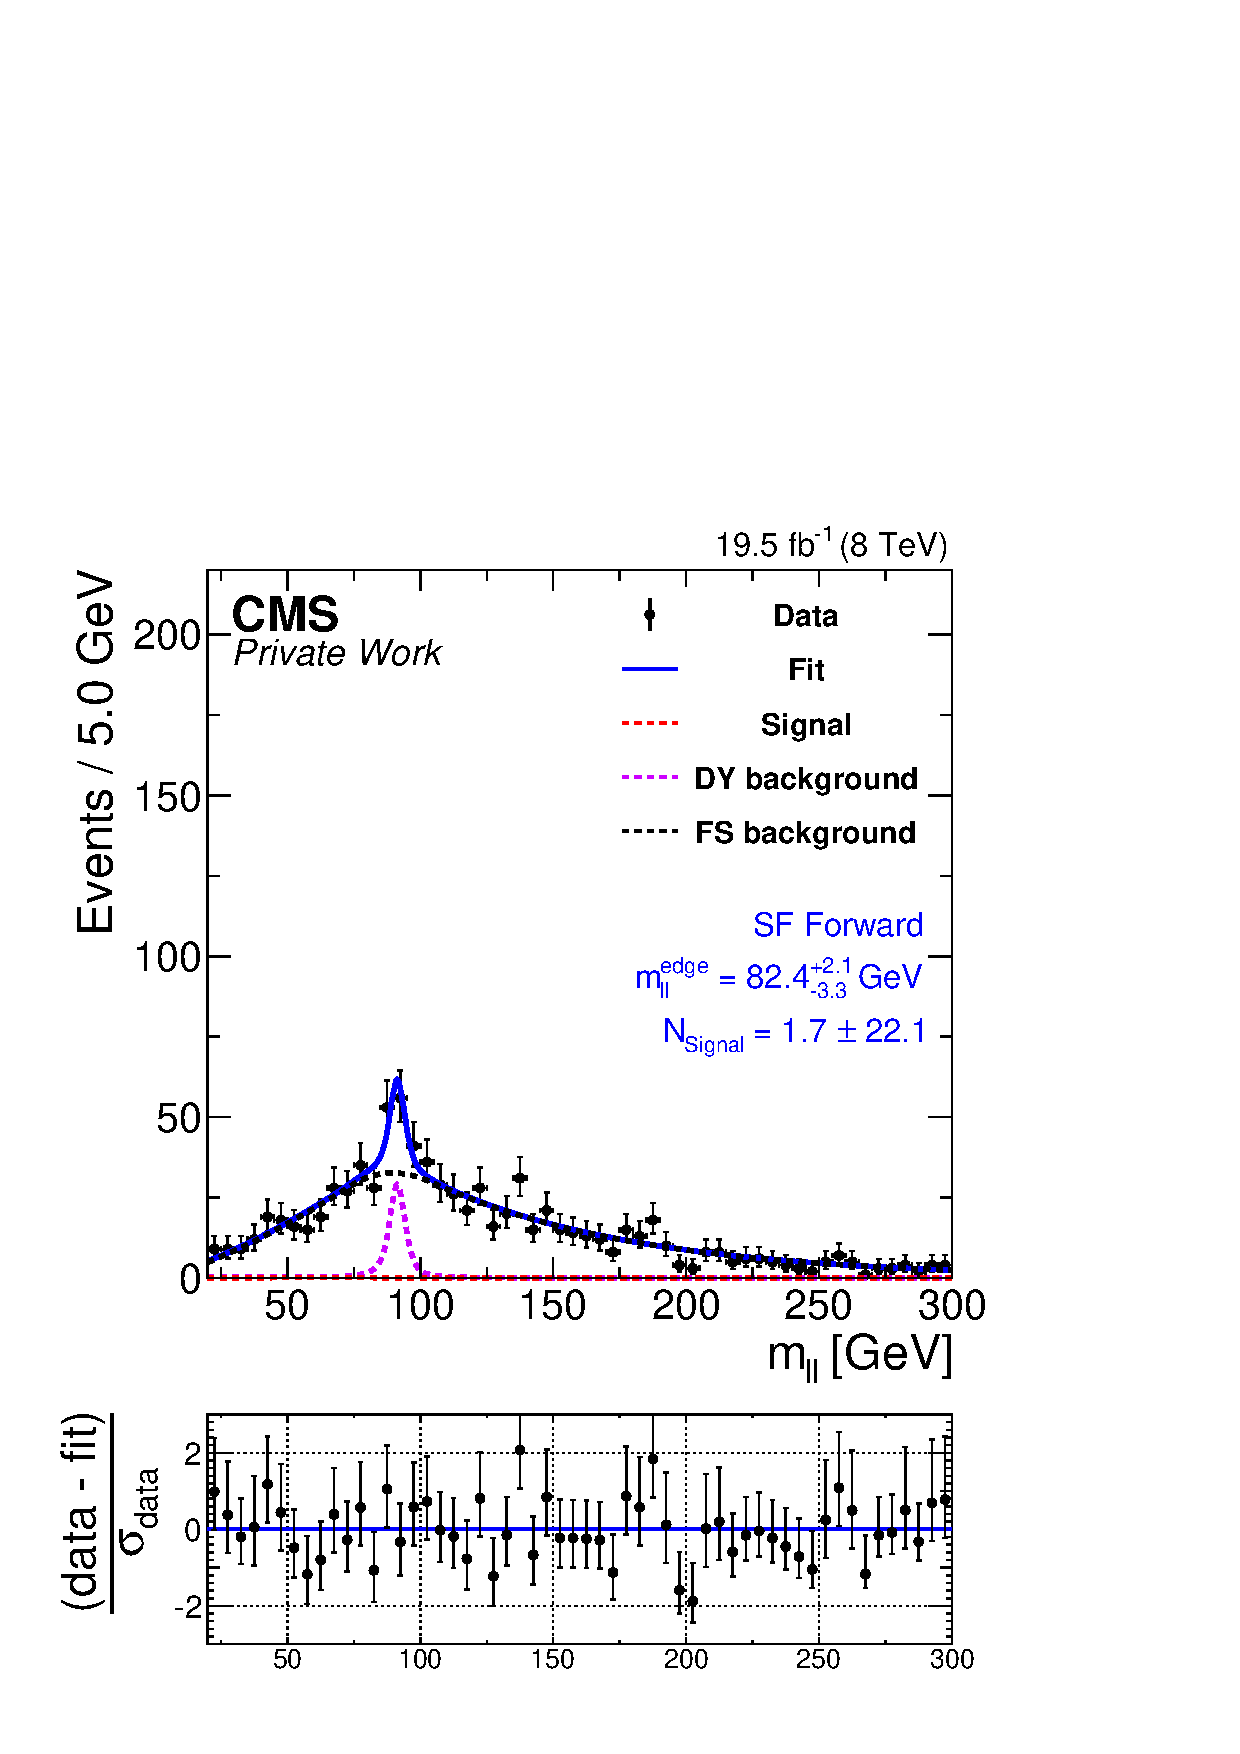
\includegraphics[width=\textwidth]{plots/results/fit/fit2012_ETHTriangle_SignalInclusive_Combined_Full2012_ETHTriangle_Forward.pdf}
  \end{minipage}
  \begin{minipage}[t]{0.49\textwidth}
    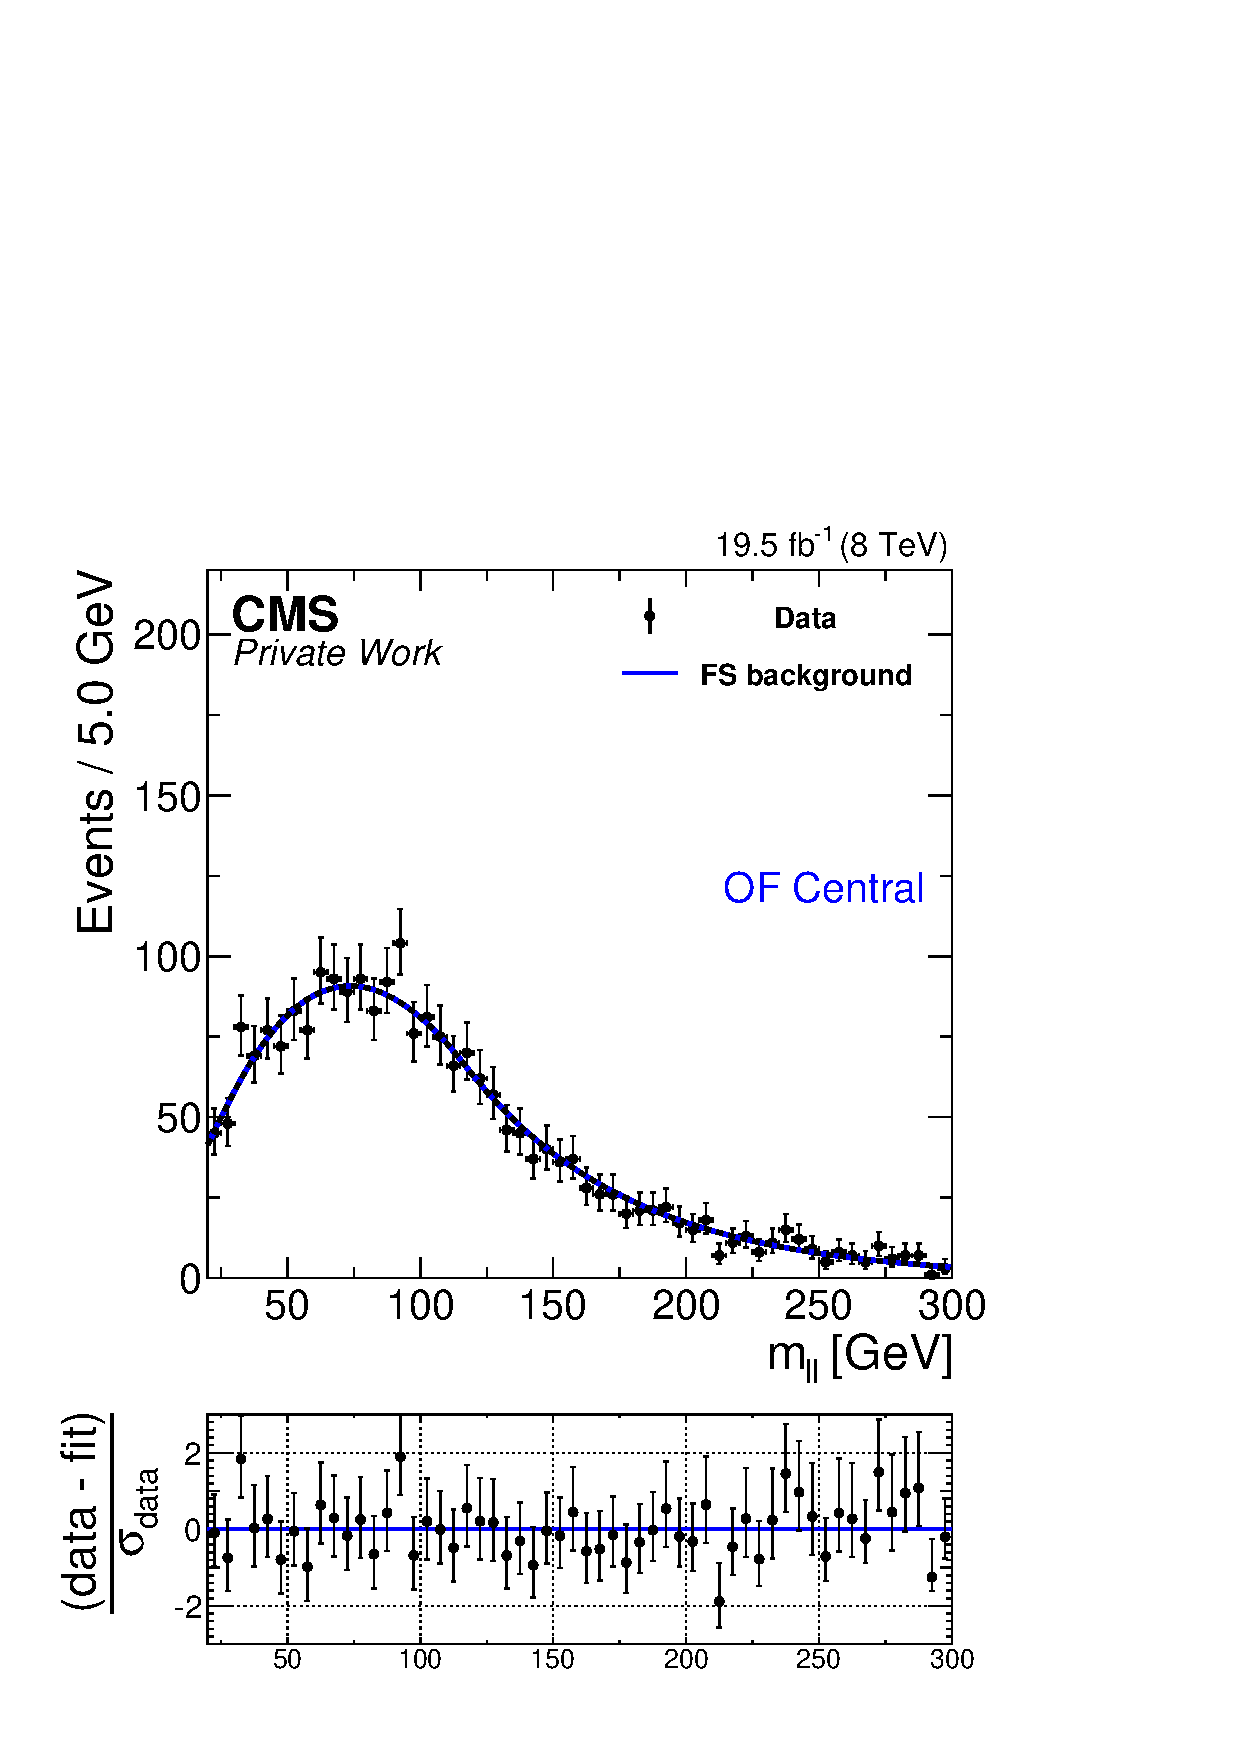
\includegraphics[width=\textwidth]{plots/results/fit/fit2012OFOS_ETHTriangle_SignalInclusive_Combined_Full2012_ETHTriangle_Central.pdf}
  \end{minipage}
  \begin{minipage}[t]{0.49\textwidth}
    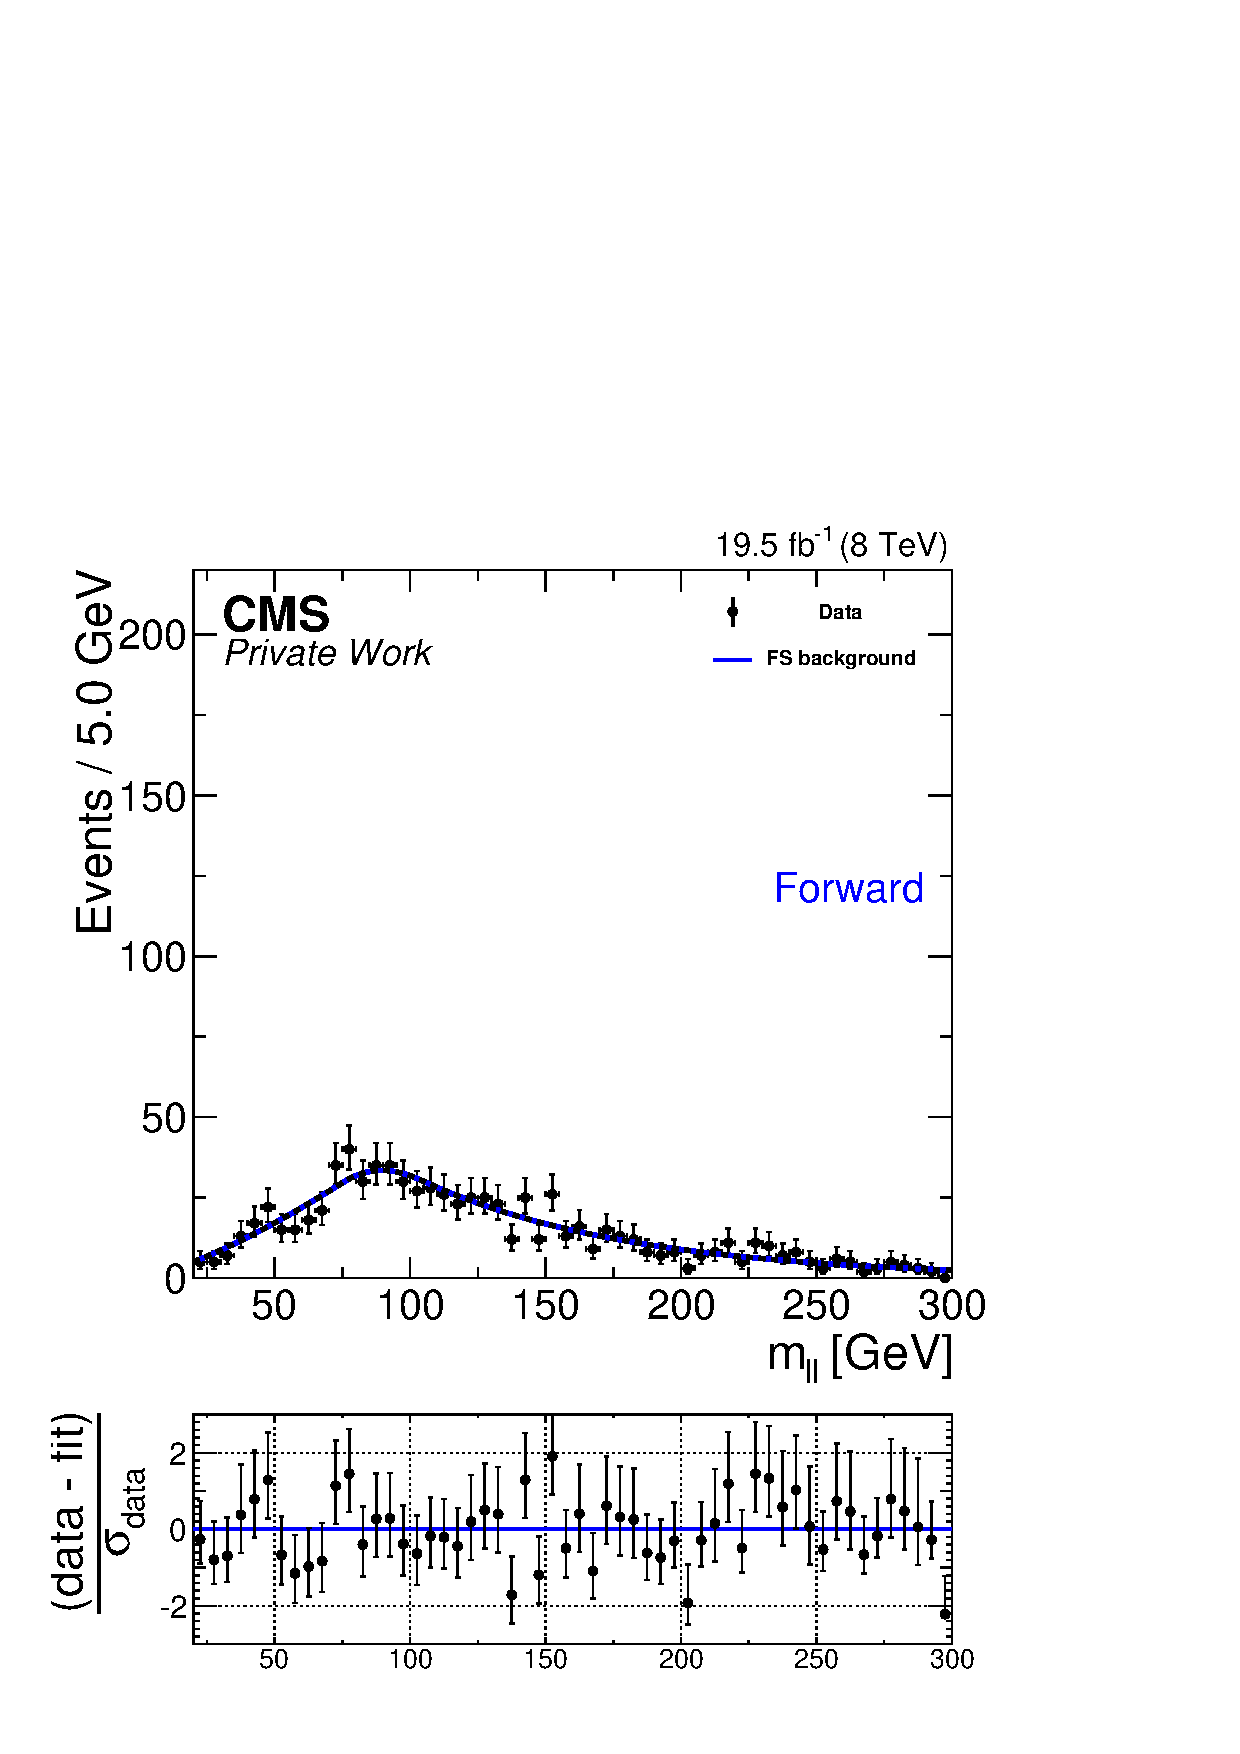
\includegraphics[width=\textwidth]{plots/results/fit/fit2012OFOS_ETHTriangle_SignalInclusive_Combined_Full2012_ETHTriangle_Forward.pdf}
  \end{minipage}
  \caption{Fit results in the signal region. Shown are the \mll distributions in SF (top) and OF (bottom) events for the central (left) and forward (right) dilepton selection. The fit is shown as a solid blue line while the different components are shown as dashed lines, the signal model in red, the Drell--Yan model in violet, and the flavour-symmetric model in black.}
  \label{fig:fit:result}
\end{figure}


\begin{table}[hbtp]
 \renewcommand{\arraystretch}{1.3}
 \setlength{\belowcaptionskip}{6pt}
 \centering
 \caption{Results of the fit in search for a kinematic edge in the signal region.
     }
  \label{tab:fitResult}
  \begin{tabular}{l| cc }
    \hline
    \hline
                                &  Central        & Forward \\ 

    \hline
        Drell--Yan background       &  170$\pm$23                   & 55$\pm$15  \\
        Flav. Sym. background in OF       &  2293$\pm$45                   & 792$\pm$25  \\
        \Rsfof       &  1.024$\pm$0.027                   & 1.012$\pm$0.042  \\
        signal events       &  140$\pm$44                   & 2$\pm$22  \\
        $m_{\ell\ell}^{edge}$ [GeV]       &  \multicolumn{2}{c}{$82.4^{+2.1}_{-3.3}$}  \\

\hline
\        local significance [$\sigma$]       &  \multicolumn{2}{c}{2.5 }  \\

    \hline
    \hline    
  \end{tabular}
\end{table}




A scan of the log-likelihood as a function of the edge position $m_{\ell\ell}^{egde}$ is shown in Figure~\ref{fig:fit:likelihoodScan}. The values have been shifted to set the minimum to zero. The curve exhibits a sharp drop at the best fit value for $m_{\ell\ell}^{egde}$, which is indeed the global minimum over the considered mass range. 

\begin{figure}[htbp]
\centering
  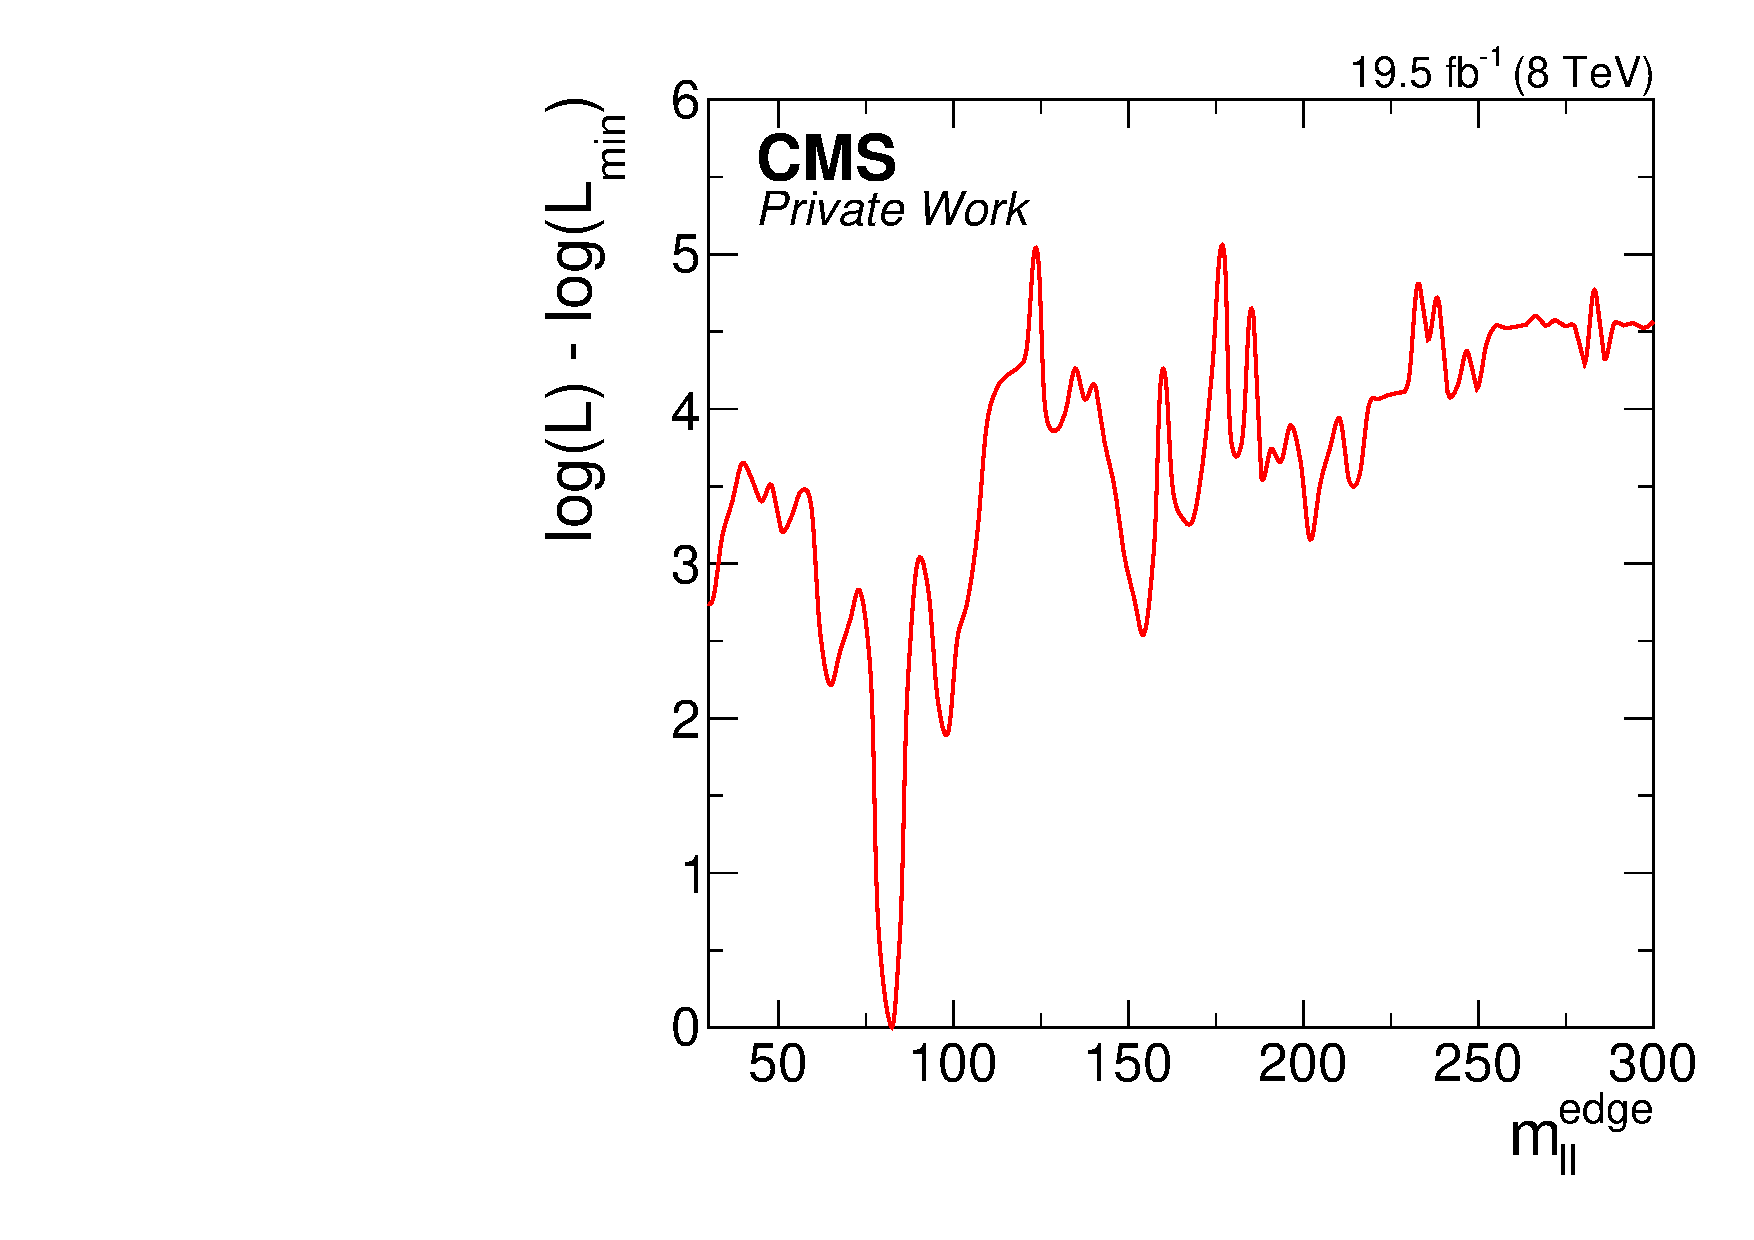
\includegraphics[width=0.6\textwidth]{plots/results/fit/signal.pdf}
\caption{Scan of the observed log-likelihood in the signal region subtracted by the minimal value as a function of $m_{\ell\ell}^{edge}$.}
\label{fig:fit:likelihoodScan}
\end{figure}

The local fit significance, for the case of a fixed edge position, is calculated applying Wilk's Theorem~\cite{wilks1938}, which states that the distribution of $-2\left(\log\left(L_1\right)-\log\left(L_0\right)\right)$ (abbreviated as $-2\Delta\left(\log\left(L\right)\right)$) is distributed as a $\chi^2$ distribution with n degrees of freedom, where n is the number of free parameters of the signal model and $L_0$ and $L_1$ are the likelihood values of the background only and the signal plus background hypothesis. The p-value of a result is obtained by integrating this $\chi^2$ distribution for values larger than the one observed in data. However, Wilk's Theorem does not hold in the cases, where one parameter of the signal model is not defined in the background only model. This is the case for signal models including the position of a bump, or in this case an edge, as a free parameter. Therefore the edge position has to be fixed when Wilk's Theorem is applied and no global significance can be obtained this way. 

The applicability of Wilk's theorem in the case of local significances is demonstrated using the toy fits described in Section~\ref{sec:toysWO}. They can also be used to calculate the significance directly and are also able to provide global results. Considered are toy dataset without signal injection. The fits are performed both with a floating edge position and fixed \mlledge. Figure~\ref{fig:fit:toySignif} shows the resulting distributions of $-2\Delta\left(\log\left(L\right)\right)$ for both scenarios. The likelihood values entering this distribution are obtained by fits of the full model described in section~\ref{sec:fullModel} for the signal plus background hypothesis and of the same model but excluding the signal model components for the background only hypothesis. The $\chi^2$ distributions for two and three degrees of freedom are shown for illustration. In the case of the fixed edge the results of the fits follow the distribution for two degrees of freedom, as expected from the presence of the free parameters $N_{S}^{\text{central}}$ and $N_{S}^{\text{forward}}$. This proves the applicability of Wilk's theorem in this case. The floating edge position, however, clearly does not simply act as an additional degree of freedom as the distribution of the toy results is shifted to higher values of $-2\Delta\left(\log\left(L\right)\right)$, indicating that Wilk's theorem does indeed not hold for this type of models.

The p-value of the fit result is in both cases given by the fraction of results for which  $-2\Delta\left(\log\left(L\right)\right)$ exceeds the one observed on data. The result for a fixed edge can then be interpreted as a local p-value while the one for a floating edge gives a global p-value taking into account the so called ``Look-elsewhere-effect''~\cite{GrossVittels}. However, as the signal yield is allowed to be negative, the resulting p-values have to be reduced by a factor of two to take into account that we only consider positive signals to have physical meaning~\cite{GrossVittels}. This corrected p-value is translated into a significance interpreting it as the one-sided tail probability of a unit-Gaussian. The resulting uncorrected p-values given the value  $-2\Delta\left(\log\left(L\right)\right)$ observed in data are $0.012^{+0.004}_{-0.003}$, corresponding to $2.5\sigma$, in the local and $0.091^{+0.009}_{-0.009}$, corresponding to $1.7\sigma$, in the global case.

\begin{figure}[htbp]
\centering
  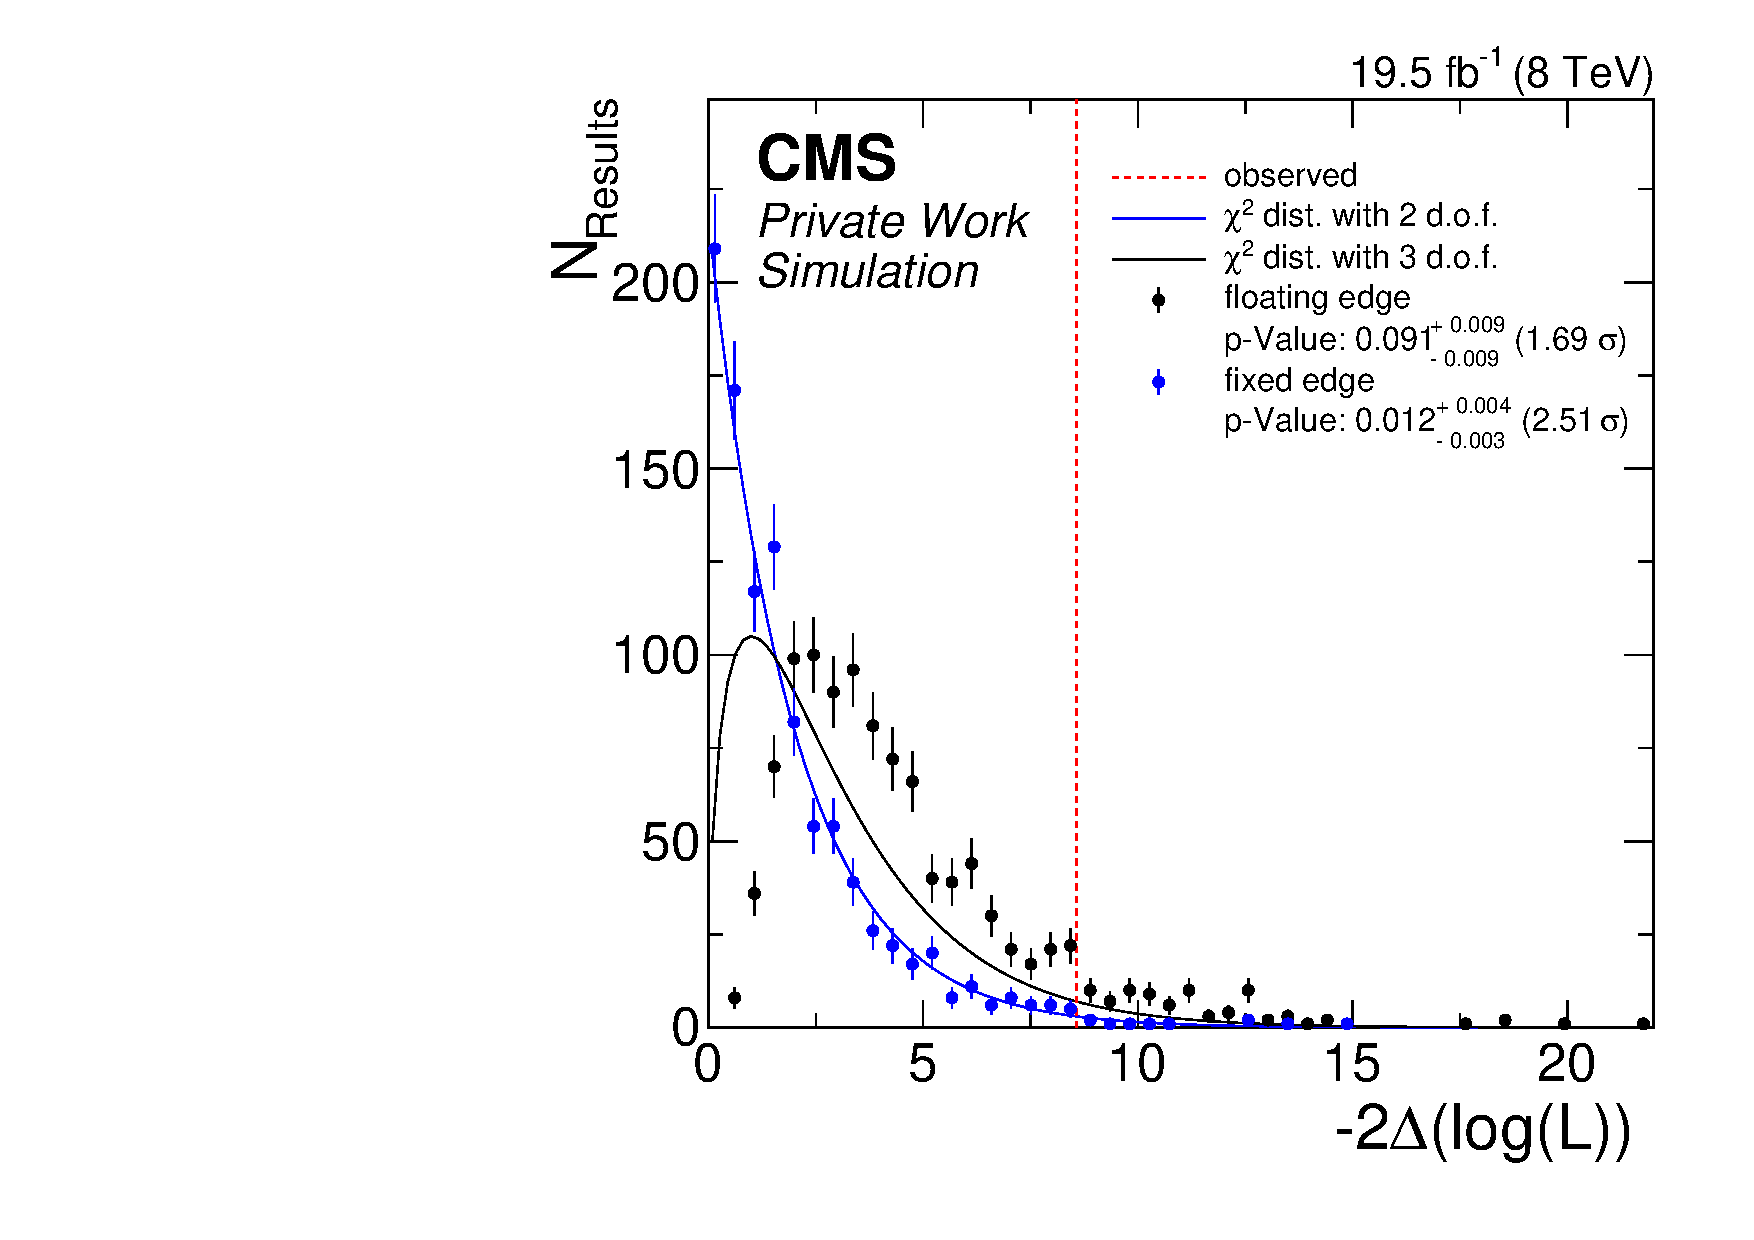
\includegraphics[width=0.6\textwidth]{plots/results/fit/toyResults/significanceStudy_BackgroundOnly.pdf}
\caption{Calculation of the fit significance using background only toy datasets. Shown are the distribution of $-2\Delta(log(L))$ for fits with floating (black) and fixed (blue) edge position. Also shown are $\chi^2$ distributions for two (blue) and three (black) degrees of freedoms. The dashed red line indicates the value of $-2\Delta(log(L))$ observed on data in case of a floating edge.}
\label{fig:fit:toySignif}
\end{figure}

As Wilk's theorem is applicable in the case of fixed edge positions, local p-values and significances can be calculated analytically from the $\chi^2$ function for two degrees of freedom. The p-value is defined as the integral of the function above the value of  $-2\Delta\left(\log\left(L\right)\right)$ observed on data for a fit performed with fixed edge position. Performing such a fit on data with \mlledge set to $\unit{82.4}{\giga\electronvolt}$, the value obtained with the fit with a floating edge position, this results in a p-value of 0.014, corresponding to a significance of $2.5\sigma$. This is well compatible with the result observed using toy datasets. The local significances reported in Table~\ref{tab:fitResult} and those discussed in the following are calculated using the analytical calculation as it is much faster and not affected by statistical uncertainties. Also, the toys have the small caveat that a different background shape than in the nominal fit is used. 

As further validation of the result on data, the results obtained with different parametrisations of the flavour-symmetric background are compared to the nominal result in Table~\ref{tab:fitComparison}. In each case first a fit has been performed with a floating edge position to find the best value for \mlledge, followed by a fit with a fixed edge at that position. The value of  $-2\Delta\left(\log\left(L\right)\right)$ obtained by the latter fit is used to calculate the local significance. For the sake of clarity, only yields in the central signal region are shown. However, similar agreement is observed in the forward signal region. In general, there is good agreement between all considered parametrisations. The best agreement is seen in the number of fitted flavour-symmetric events in the OF sample, which is expected, as here the fit is most simple, consisting only of the shape for flavour-symmetric backgrounds. Good agreement is also observed for $m_{\ell\ell}^{egde}$ and the number of signal events, which are stable against the choice of the background model. The largest differences are observed for \Rsfof and the yield of the Drell--Yan model, which the fit can trade off against each other, depending on the parametrisation of the flavour-symmetric background. Here, the largest deviations are observed for the shape used in the analysis of the $\unit{7}{\tera\electronvolt}$ dataset. As this shape is known to not satisfactorily described the flavour-symmetric background, it is encouraging to see that the fit result is stable against such biases. The observed local significance is very similar among all analytical parametrisations. In the case of the KDE and the binned parametrisation, the shape of the distribution is not free in the fit, as discussed above, excluding the statistical uncertainty on this shape from the fit and resulting in a systematically larger local significance. 


\begin{table}[hbtp]
 \renewcommand{\arraystretch}{1.3}
 \setlength{\belowcaptionskip}{6pt}
 \centering
 \caption{Comparison of edge fit results in the signal region for different parametrizations of the flavour-symmetric background. Results are given for the central signal region only. Similar agreement between the parametrization is also observed in the forward signal region.
     }
  \label{tab:fitComparison}
  \begin{tabular}{l| c c c c c c }
    \hline
    \hline
                                &  $N_{DY}$  & $N_{FS}$ & \Rsfof & $N_{S}$ &  $m_{\ell\ell}^{edge}$ [GeV]  & local $\sigma$ \\ 

    \hline
        nominal       &  170$\pm$23  &  2293$\pm$45 &  1.024$\pm$0.027 &  140$\pm$43 &   $82.4^{+2.1}_{-3.3}$      & 2.5  \\
        sum of Gaussians       &  168$\pm$24  &  2292$\pm$44 &  1.023$\pm$0.027 &  146$\pm$50 &   $82.1^{+2.2}_{-3.7}$      & 2.7  \\
        kernel density estimation       &  154$\pm$22  &  2296$\pm$43 &  1.028$\pm$0.026 &  141$\pm$41 &   $81.7^{+2.3}_{-3.4}$      & 3.1  \\
        histogram       &  140$\pm$23  &  2296$\pm$43 &  1.029$\pm$0.026 &  153$\pm$41 &   $83.0^{+1.7}_{-2.4}$      & 3.5  \\
        2011 shape       &  181$\pm$23  &  2290$\pm$43 &  1.020$\pm$0.026 &  146$\pm$46 &   $82.8^{+1.9}_{-2.5}$      & 2.7  \\

    \hline
    \hline    
  \end{tabular}
\end{table}




To compare the fit result with that of the counting experiment, the fitted event yields in the low-mass region ($\unit{20}{\giga\electronvolt} < \mll < \unit{70}{\giga\electronvolt}$) for central dilepton events have been derived separately for the two background models and the signal. They are shown in Table~\ref{tab:fitResultLowMass} and compared to the background predictions and the observed signal yield of the counting experiment in that region. Also, the fitted yield for Drell--Yan backgrounds  in the on-\Z region ($\unit{81}{\giga\electronvolt} < \mll < \unit{101}{\giga\electronvolt}$) is compared to the prediction from the JZB and \MET templates methods. In this case, the fitted Drell--Yan yield exceeds the prediction by 26 events, a difference that is well covered by the respective uncertainties. In the low-mass region good agreement between counting experiment and fit is observed, also. The Drell--Yan background is again fitted higher than expected from the prediction, as the ratio between the off-shell component and the peak is fixed and the normalisation of this model is determined dominantly on the Z boson peak. In the fit the contribution of flavour-symmetric backgrounds is increased, caused by the increased value of \Rsfof. This is reflected in a fitted signal yield that is 11 events lower than in the counting experiment. For all considered components the use of shape information has allowed for reduced uncertainties on the event yields, most notably on the yield for flavour-symmetric backgrounds. 


\begin{table}[hbtp]
 \renewcommand{\arraystretch}{1.3}
 \setlength{\belowcaptionskip}{6pt}
 \centering
 \caption{Comparison of the fit result and the result of the counting experiment in the low mass region for central leptons. The probability density functions contributing to the fit model are integrated in the region $20 < \mll < 70$\GeV to obtain the fitted yields in this interval. Also, the yield in the on-\Z region is calculated and compared to the prediction. 
     }
  \label{tab:fitResultLowMass}
  \begin{tabular}{l| cc }
    \hline
    \hline
                                &  Fit        & Counting experiment \\ 

    \hline
    \multicolumn{3}{c}{on-\Z region} \\ 

    \hline
        Drell--Yan background       &  145$\pm$19                   & 119$\pm$21  \\

\hline
    \multicolumn{3}{c}{low-mass region} \\ 

    \hline
        Drell--Yan background       &  10$\pm$1                   & 8$\pm$2  \\
        Flav. Sym. background       &  760$\pm$14                   & 746$\pm$37  \\
        signal events       &  98$\pm$30                   & 109$\pm$48  \\

    \hline
    \hline    
  \end{tabular}
\end{table}


